% $Id: Note_ResFit_Main.tex,v 1.13 2010/10/08 07:52:27 mschrode Exp $

% =====  HEADER  ========================================

% ----- Document ----------------------------------------
\documentclass[a4paper]{cmspaper} %USE for CMS machines


% ----- User defined commands ---------------------------
% $ Id: $

% Required pacakges
\usepackage{amsmath}
\usepackage{cancel}
\usepackage{xspace}

% Sectioning
\newcommand{\qsec}[1]{Section~\ref{#1}}
\newcommand{\qfig}[1]{Fig.~\ref{#1}}
\newcommand{\qtab}[1]{Table~\ref{#1}}
\newcommand{\qeq}[1]{\eqref{#1}}

% Units
\newcommand{\tev}{\ensuremath{\;\text{Te}\kern-0.06667em\text{V}}\xspace}
\newcommand{\gev}{\ensuremath{\;\text{Ge}\kern-0.06667em\text{V}}\xspace}
\newcommand{\mev}{\ensuremath{\;\text{Me}\kern-0.06667em\text{V}}\xspace}
\newcommand{\km}{\ensuremath{\;\text{km}}\xspace}
\newcommand{\m}{\ensuremath{\;\text{m}}\xspace}
\newcommand{\cm}{\ensuremath{\;\text{cm}}\xspace}
\newcommand{\mm}{\ensuremath{\;\text{mm}}\xspace}
\newcommand{\second}{\ensuremath{\;\text{s}}\xspace}
\newcommand{\tons}{\ensuremath{\;\text{t}}\xspace}
\newcommand{\tesla}{\ensuremath{\;\text{T}}\xspace}
\newcommand{\kelvin}{\ensuremath{\;\text{K}}\xspace}
\newcommand{\pbinv}{\ensuremath{\;\text{pb}^{-1}}\xspace}

% Quantities
\newcommand{\et}{\ensuremath{E_{\text{T}}}\xspace}
\newcommand{\met}{\ensuremath{\slash\mkern-12mu{E}_{\text{T}}}\xspace}
\newcommand{\mht}{\ensuremath{\slash\mkern-12mu{H}_{\text{T}}}\xspace}
\newcommand{\metvec}{\ensuremath{\slash\mkern-12mu{\vec{E}}_{\text{T}}}\xspace}
\newcommand{\pt}{\ensuremath{p_{\text{T}}}\xspace}
\newcommand{\pti}[1]{\ensuremath{p_{\text{T},#1}}\xspace}
\newcommand{\ptvec}{\ensuremath{\vec{p}_{\text{T}}}\xspace}
\newcommand{\ptsub}[1]{\ensuremath{p_{\text{T},#1}}\xspace}
\newcommand{\ptvecsub}[1]{\ensuremath{\vec{p}_{\text{T},#1}}\xspace}
\newcommand{\ptdijet}{\ensuremath{p^{\text{dijet}}_{\text{T}}}\xspace}
\newcommand{\ptgen}{\ensuremath{p^{\text{gen}}_{\text{T}}}\xspace}
\newcommand{\pthat}{\ensuremath{\hat{p}_{\text{T}}}\xspace}
\newcommand{\pttrue}{\ensuremath{p^{\text{true}}_{\text{T}}}\xspace}
\newcommand{\pttruehigh}[1]{\ensuremath{p^{\text{true,#1}}_{\text{T}}}\xspace}
\newcommand{\ptrel}{\ensuremath{p^{\text{rel}}_{\text{T},3}}\xspace}
\newcommand{\ptmeas}{\ensuremath{p^{\text{meas}}_{\text{T}}}\xspace}
\newcommand{\ptmeasi}[1]{\ensuremath{p^{\text{meas}}_{\text{T},#1}}\xspace}
\newcommand{\ptcalo}{\ensuremath{p^{\text{calo}}_{\text{T}}}\xspace}
\newcommand{\ptcaloi}[1]{\ensuremath{p^{\text{calo}}_{\text{T},#1}}\xspace}
\newcommand{\ptmin}{\ensuremath{\pt^{\text{min}}}\xspace}
\newcommand{\ptmax}{\ensuremath{\pt^{\text{max}}}\xspace}
\newcommand{\ptparticle}{\ensuremath{\pt(\text{particle})}\xspace}
\newcommand{\ptreco}{\ensuremath{\pt(\text{reco})}\xspace}

% Symbols
\newcommand{\dif}[1]{\ensuremath{\text{d}#1}\xspace}
\newcommand{\e}{\,\text{e}}
\newcommand{\nup}[1]{$^{\text{\scriptsize #1}}$}
\newcommand{\dgr}{\ensuremath{\,^{\circ}}}
\newcommand{\mean}[1]{\ensuremath{\langle#1\rangle}}
\newcommand{\gqq}[1]{\ensuremath{\glqq#1\grqq}}
\newcommand{\rarr}{\ensuremath{\rightarrow}\xspace}

% Words and characters
\newcommand{\diagonalsout}[1]{\ensuremath{\cancel{\text{#1}}}}
\newcommand{\genjet}{GenJet\xspace}
\newcommand{\genjets}{GenJets\xspace}
\newcommand{\calojet}{CaloJet\xspace}
\newcommand{\calojets}{CaloJets\xspace}




% ----- Additional packages -----------------------------
\usepackage{subfigure}
\usepackage{booktabs}
\usepackage{multirow}


% ----- pdflatex setup ----------------------------------
\usepackage[pdftex]{color,graphicx}
\usepackage[pdftex]{hyperref}
\hypersetup{unicode=true}
\hypersetup{bookmarks=true}
\hypersetup{pdftitle={Determination of the Jet Energy Resolution in QCD Dijet Events}}
\hypersetup{pdfauthor={Matthias Schr\"oder}}
\hypersetup{colorlinks=true}



% =====  DOCUMENT  ======================================

\begin{document}


% ----- Title page and TOC ------------------------------
\begin{titlepage}
  \date{\today}
  \title{Measurement of the Jet \pt Response Function in QCD Dijet
    Events using an Unbinned Maximum Likelihood Method}
  \begin{abstract}
    Analysing jet final states is an important way to investigate
    Standard Model and beyond processes and requires a precise
    knowledge of the jet transverse momentum, \textit{\pt}, resolution.	
    A method to determine the resolution from QCD dijet
    events is presented using an unbinned maximum
    likelihood fit of the \pt asymmetry.
    In this way, determination of the full response function incl. non-Gaussian
    tails and correction for selection biases is possible.
    Dijet events have a large cross section and hence provide a
    high \pt reach and an early sensitivity to tails.
    So far, a measurement of the Gaussian response has been performed
    on a sample of Collider data corresponding to an integrated luminosity of $2.2\pbinv$.
	
  \end{abstract}
\end{titlepage}
\tableofcontents


% ----- Main part from external files -------------------
% $Id: Note_ResFit_Introduction.tex,v 1.4 2010/06/01 17:24:50 mschrode Exp $


\section{Introduction}

The analysis of jet final states provides an important way to investigate Standard Model and beyond processes and requires a precise knowledge of the jet transverse momentum, \textit{\pt}, resolution.

In this note the jet response, \textit{R}, is defined as the ratio of the measured detector level jet \pt and the underlying particle level jet \pt, \textit{\ptparticle}.
The jet response distribution for a constant \ptparticle follows a Gaussian in good approximation.
Therefore the jet resolution is defined as the standard deviation of the jet response distribution at a given \ptparticle.

\textit{
\begin{itemize}
\item Gaussian core: calorimeter measurement
\item Low tail: punch-through; $\mu$, $\nu$ from heavy flavour jets
\item High tail: non-linearities of calorimeter
\end{itemize}
}

In this note a method is presented to derive the jet transverse momentum, \pt, resolution from QCD dijet events in collider data.
Dijet events have a large cross section e.g. in comparison to $\gamma$-jet events and hence provide a higher \pt reach and an early sensitivity also to non-Gaussian tails of the jet response function.

A likelihood function is constructed with probability densities, \textit{pdf}s, of the \pt imbalance in the dijet event.
The pdfs are a convolution of the particle level jet differential cross section with suitable parameterisations of the jet \pt response functions.
As a consequence, the measured resolution is parametrised as a function of particle level jet \pt.
In addition, a description of selection biases arising from requirements on the measured jet \pt is incorporated.

The method is strictly valid in the ideal case of events with only two jets in the final state, that are balanced in \pt at the particle level, and under the assumption that detector response and resolution effects on both jets are not correlated with each other.
In real QCD events, however, the \pt balance of the two jets is affected by the presence of additional jet activity from e.g. gluon radiation and the measurement has to be corrected for this effect.

In case that other event types are included into the likelihood, such as $\gamma+$jets, suitable probability density functions must be defined.

The studies included in this note are performed on jets that have been reconstructed from calorimeter towers, \textit{\calojets}, although the method is general and may be applied to any type of detector level jet.


% $Id: Note_ResFit_Technique.tex,v 1.3 2010/05/31 13:10:51 mschrode Exp $


\section{Description of the Method}\label{sec:ResFit:Method}

\subsection{Definition of the dijet likelihood}\label{sec:ResFit:Method:Likelihood}

The underlying assumptions of the presented method are
\begin{itemize}
\item an ideal dijet event configuration with exactly two jets that
  are balanced in true transverse momentum, \mbox{$\pttrue\equiv\ptparticle$};
\item measured jet transverse momenta,
  \mbox{$\ptmeasi{i}\equiv\ptcaloi{i}$}, $i\in[1,2]$, result from uncorrelated
  calorimeter measurements.
\end{itemize}
Based on these, the pdf of a measured dijet event configuration is defined as
\begin{equation}
  \label{eq:resFit:DijetPdf}
  g_{\mathbf{\xi}}\left(\ptmeasi{1},\ptmeasi{2}\right) \propto \int^{\infty}_{0}\dif{\pttrue}\,f\left(\pttrue\right)
  \cdot r_{\mathbf{\xi}}\left(\ptmeasi{1}|\pttrue\right)
  \cdot r_{\mathbf{\xi}}\left(\ptmeasi{2}|\pttrue\right).
\end{equation}
Here,
\begin{itemize}
\item $f(\pttrue)$ denotes the pdf of the true jet \pt
  i.e. the particle level differential dijet cross section.
  In the following it is assumed to be known
  and taken from the Monte Carlo simulation
  (comp. e.g. Fig.~\ref{fig:resFit:qcd:dijetspectrum:subA}).
  Uncertainties on the simulated cross section have to be propagated to
  the measured resolution and added as a systematic uncertainty of the
  method, which is in fact small as shown in Section~\ref{};
\item $r_{\mathbf{\xi}}(\ptmeasi{i}|\pttrue)$ denotes the pdf of the measured \pt
  of the $i$-th jet.
  It is parametrised with a suitable function depending on the set of
  parameters $\mathbf{\xi}$, e.g. a Gauss or Crystal Ball function.
\end{itemize}
It is important to note that
$g_{\mathbf{\xi}}(\ptmeasi{1},\ptmeasi{2})$ does not depend on \pttrue
as this is the integration variable.

If $f(\pttrue)$ and $r_{\mathbf{\xi}}(\ptmeasi{i}|\pttrue)$ are properly normalised in the considered interval \mbox{$\pttruehigh{min} < \pttrue < \pttruehigh{max}$} such that
\begin{eqnarray*}
  1 & = & \int^{\pttruehigh{max}}_{\pttruehigh{max}}\dif{\pttrue}\,f\left(\pttrue\right) \\
  1 & = & \int^{\infty}_{0}\dif{\ptmeasi{i}}\,r_{\mathbf{\xi}}\left(\ptmeasi{i}|\pttrue\right)
\end{eqnarray*}
then also the dijet pdf is properly normalised to
\begin{equation*}
  1 = \int^{\infty}_{0}\dif{\ptmeasi{1}}\,\int^{\infty}_{0}\dif{\ptmeasi{2}}\, g_{\mathbf{\xi}}\left(\ptmeasi{1},\ptmeasi{2}\right),
\end{equation*}
provided the integration order of $\ptmeasi{i}$ and $\pttrue$ can be interchanged.

For a sample of $N$ dijet events, a likelihood is defined as
\begin{equation}
  \label{eq:ResFit:Likelihood}
  \mathcal{L}\left(\mathbf{\xi}\right) = \prod^{N}_{k=1} g_{\mathbf{\xi},k}\left(\ptmeasi{1},\ptmeasi{2}\right).
\end{equation}
Maximisation of $\mathcal{L}(\mathbf{\xi})$ then results in an
estimate of the optimal values of $\mathbf{\xi}$ for the chosen
function $r_{\mathbf{\xi}}(\ptmeasi{i}|\pttrue)$.
Note that $r_{\mathbf{\xi}}(\ptmeasi{i}|\pttrue)$ is defined as the
pdf of the measured jet \pt.
The pdf of the jet \pt response \mbox{$R_{i}\equiv\ptmeasi{i} / \pttrue$} is obtained by parameter transformation
\begin{equation*}
  r_{\mathbf{\xi}}\left(R_{i}|\pttrue\right) =
  r_{\mathbf{\xi}}\left(\ptmeasi{i}\left(R_{i}\right)|\pttrue\right)\cdot\left|\frac{\dif{\ptmeasi{i}}}{\dif{R_{i}}}\right|.
\end{equation*}



\subsection{Description of selection biases in a data driven event selection}\label{sec:ResFit:Method:Biases}

\textit{To be copied from RA2 note}

\section{Samples and Event Selection}\label{sec:ResFit:EvtSel}

A sample of QCD events corresponding to an integrated luminosity of $2.2\pbinv$ is
selected from the data set \texttt{JetMET\_Run2010A-PromptReco-v4}, which has been reconstructed with the \texttt{3\_6\_1\_patch7} version of the \texttt{CMSSW} software.
The data has been collected by triggering on the minimum average uncorrected transverse momentum, \mbox{$\ptave = (\pti{1} + \pti{2})/2$}, of the leading two jets in each event (\texttt{HLT\_DiJetAve15U}, \texttt{HLT\_DiJetAve50U}).
The different trigger thresholds are given in \qtab{tab:ResFit:PtAveBins}, for a listing of the trigger turn-on compare \eg~\cite{bib:cmspas:trigger}.
Events originating from beam-halo and other beam-background processes are rejected~\cite{bib:cmspas:monster} and a good reconstructed primary vertex is required~\cite{bib:cmspas:vertex}.

\begin{table}[ht]
  \caption{\ptave bins and applied trigger thresholds.}
  \centering
  \begin{tabular}[ht]{ccc}
    \toprule
    Bin & \ptave range (\gevnospace) & Trigger threshold \\
    &  & (uncorrected \ptave (\gevnospace)) \\
    \midrule
    1 & 60 -- 80 & 15 \\
    2 & 80 -- 100 & 80 \\
    3 & 100 -- 120 & 80 \\
    4 & 120 -- 140 & 80 \\
    5 & 140 -- 170 & 80 \\
    6 & 170 -- 200 & 80 \\
    7 & 200 -- 250 & 80 \\
    \bottomrule
  \end{tabular}
  \label{tab:ResFit:PtAveBins}
\end{table}

In order to estimate the particle level jet \pt spectrum and for closure tests, also simulated QCD multijet events are used.
They have been generated in bins of \pthat with PYTHIA6~\cite{bib:pythia} and processed through the full GEANT4~\cite{bib:geant} based CMS detector simulation (\texttt{/QCDDiJet\_PtXXtoXX/Spring10-START3X\_V26\_S09-v1/GEN-SIM-RECO}).

Jets are reconstructed from calorimeter towers using the
anti-$k_{T}$ jet clustering algorithm~\cite{bib:akj} with parameter size \mbox{$d=0.5$}.
Jet energy corrections~\cite{bib:cmspas:jec} are applied to remove the 
$\eta$ and \pt dependence of the jet energy scale (Spring10 \texttt{L2L3} corrections) and quality criteria rejecting jets clustered from detector noise~\cite{bib:cmspas:jetid} are applied to the
two leading jets (loose Jet-ID).
In order to select dijet events, the two leading jets are required to be
back-to-back in the transverse plane, \mbox{$|\Delta\phi_{i}| > 2.7$} for \mbox{$i=1,2$}.
Additionally they have to lie within the same pseudorapidity range \mbox{$|\eta_{i}| < 1.3$}.
This accounts for the dependence of the jet \pt response on $\eta$ due to the fact that the intrinsic calorimeter resolution is energy rather than \pt dependent as well as the varying calorimeter resolution in different pseudorapidity regions.

As discussed in \qsec{sec:ResFit:DataDriven:AddJets:Extrapolation}, events are further selected in bins of \ptave (\qtab{tab:ResFit:PtAveBins}) and events with additional jet activity are rejected in course of the analysis.
In case of the simulated samples, only events from a limited number of \pthat bins contribute to a given \ptave bin.
They are weighted in such a way that the realistic QCD \pt spectrum is preserved and the event weight in the lowest of these \pthat bins is one, thus achieving the maximally possible statistical precision.

\section{Application to Collider Data}\label{sec:ResFit:DataDriven}

In the following, the resolution measurement in Collider data is
discussed.

In \qsec{sec:ResFit:DataDriven:SimpleFit}, the performance of the unbinned
method is compared to a binned fit of the histogram of the dijet asymmetry.
The completely analogue case is demonstrated in
\qsec{sec:ResFit:DataDriven:SimpleFit}, where the likelihood is simplified by replacing the spectrum
with the assumption \mbox{$\pttrue = \ptave$}.
Since the unbinned fit is more sensitive to non-Gaussian tails, an outlier
suppression technique is introduced.
In \qsec{sec:ResFit:DataDriven:FullFit}, the full dijet pdf, including an assumption for the
spectrum and a description of selection biases, is finally used to fit the asymmetry;
the spectrum is also used to derive a better estimator for \ptgen.

As discussed in \qsec{sec:ResFit:DataDriven:AddJets}, additional jets in the events, \eg from soft gluon radiation, as
well as out-of-cone effects during the jet clustering bias the dijet asymmetry and have to be
corrected for when measuring the resolution.
The contributions to the bias are investigated in detail in \qsec{sec:ResFit:DataDriven:AddJets:Contributions} and
in \qsec{sec:ResFit:DataDriven:AddJets:Extrapolation} a correction method is presented using an extrapolation of
the resolution to the ideal two jet case.


\subsection{Fit of the Dijet Asymmetry}\label{sec:ResFit:DataDriven:Asym}

The dijet asymmetry is defined as
\begin{equation}\label{eq:ResFit:Asymmetry}
  A = \frac{\pti{1'}-\pti{2'}}{\pti{1'}+\pti{2'}},
\end{equation}
where \pti{1'} and \pti{2'} refer to the randomly ordered transverse momenta of the
leading two jets in an event.
In case of events with exactly two jets of same particle level jet
transverse momentum \pt and Gaussian response, the width $\sigma(A)$ of the asymmetry distribution is
related to the jet \pt resolution $\sigma$ by
\begin{equation}
  \label{eq:ResFit:ResFromAsym}
  \sigma(A) = \frac{1}{\sqrt{2}}\frac{\sigma}{\pt} \; .
\end{equation}


\subsubsection{Simple Maximum Likelihood Fit and Outlier Treatment}\label{sec:ResFit:DataDriven:SimpleFit}

If the spectrum $f$ in the dijet pdf~\qeq{eq:ResFit:DijetPdfTransformed} is replaced by \mbox{$f(\pttrue)  = \delta\left(\pttrue - \ptave\right)$}, \ie assuming \mbox{$\pttrue = \ptave$}, 
\qeq{eq:ResFit:DijetPdfTransformed} simplifies to
\begin{equation}
\label{eq:ResFit::DijetPdfTransformed:Simple}
  g_{\sigma'}\left(\Delta\pt\right) \propto
  \e^{-\frac{1}{2}\left(\frac{\Delta\pt}{\sigma'}\right)^{2}}, 
\end{equation}
with \mbox{$\sigma' = \sigma/\sqrt{2}$}.
This corresponds to the pdf of the asymmetry in the event, assuming
Gaussian response.

\begin{figure}[ht]
 \centering
  \begin{tabular}{cc}
    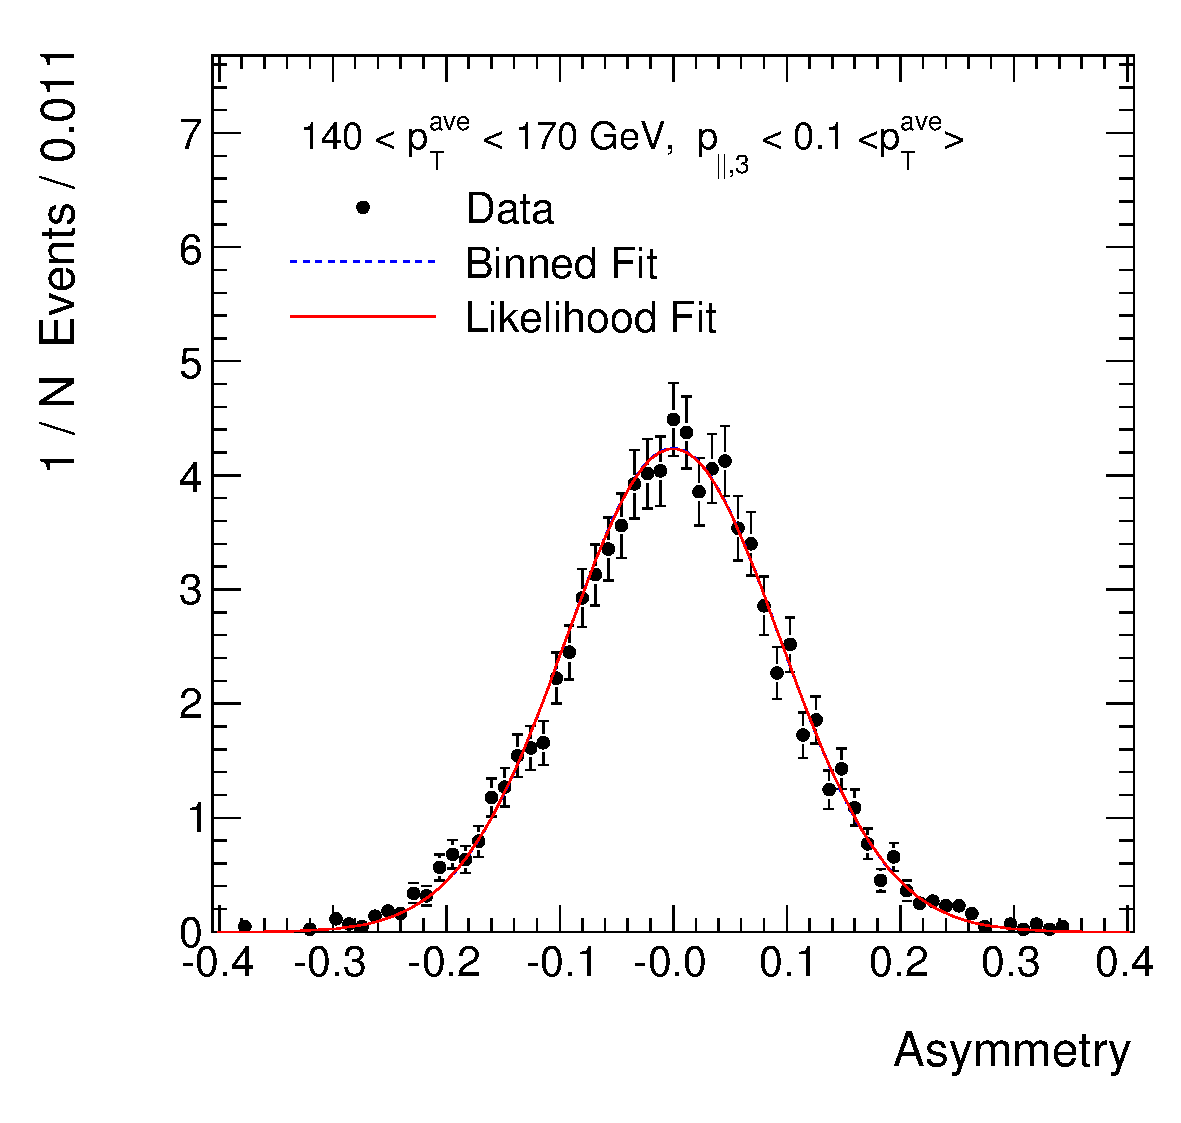
\includegraphics[width=0.45\textwidth]{figures/MaxLikeSimple_Data132440-144011_Eta00-13_PtAsymmetry_PtBin4_Pt3Cut3} &
    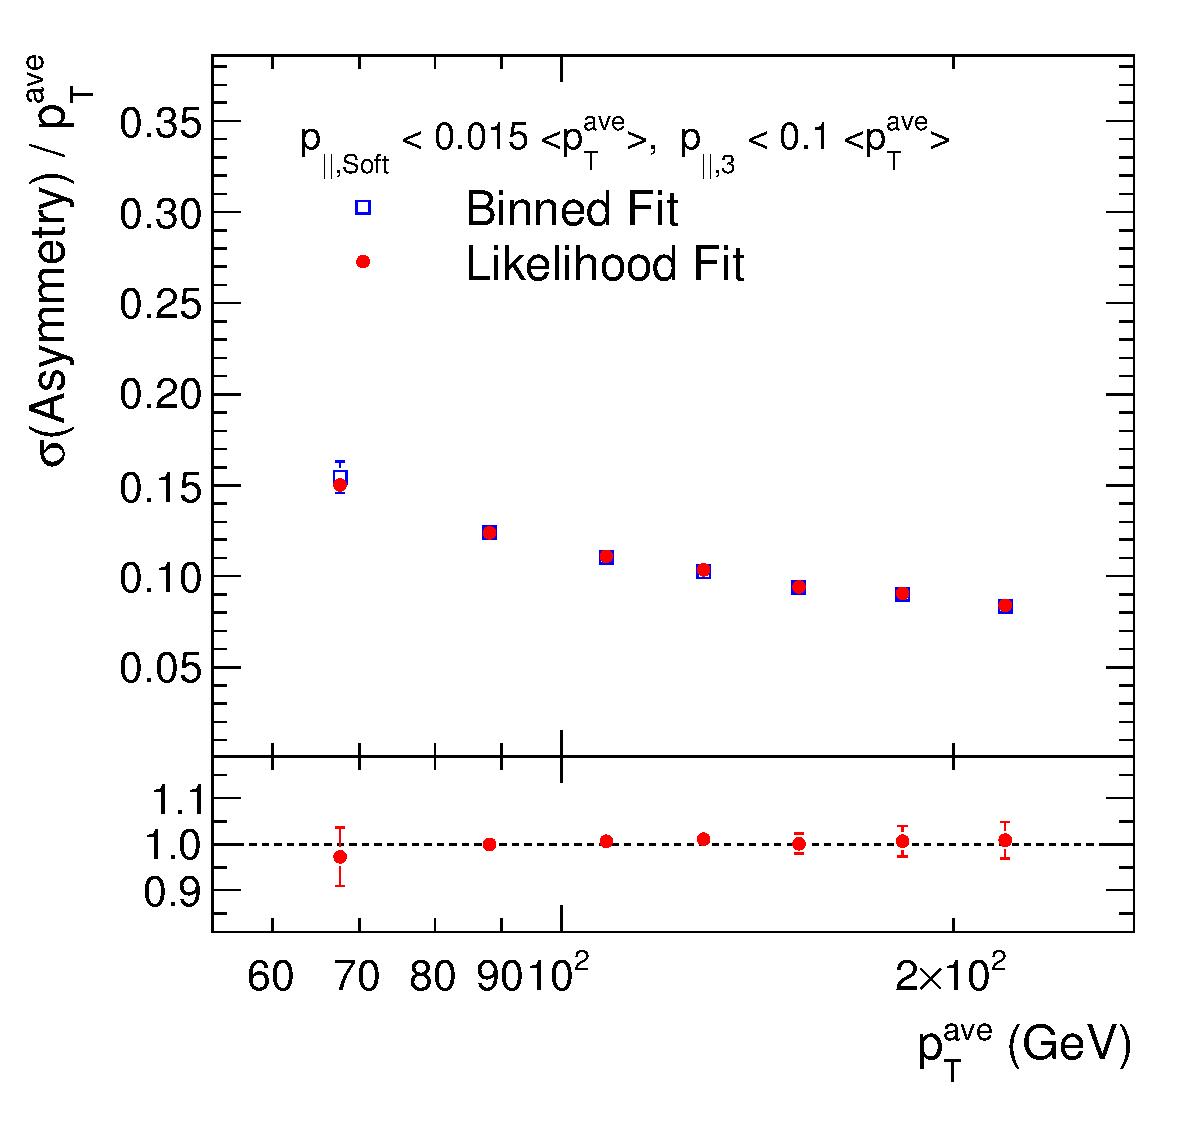
\includegraphics[width=0.45\textwidth]{figures/MaxLikeSimple_Data132440-144011_Eta00-13_PtAsymmetryWidthBottomRatio_Pt3Cut3} \\
\end{tabular}
 \caption{(\textit{Left}) Dijet asymmetry distribution measured in
    Collider data (solid circles) for \mbox{$140 < \ptave < 170\gev$}.
    It is well described by the prediction (solid line) from the
    simplified unbinned maximum likelihood fit and there is good agreement to a direct binned
    fit (dashed line) of the histogram.
    Note that both lines lie in fact on top of each other.
    (\textit{Right}) Gaussian widths of the asymmetry distributions in
    Collider data from binned fits of the
    histograms (open squares) in comparison to the results from
    the unbinned fit (solid circles) in different \ptave bins.}
  \label{fig:ResFit:DataDriven:Simple}
\end{figure}

In real data, however, there are non-Gaussian tails biasing the fit of the asymmetry.
In case of a binned fit of the histogram, the influence of the tails is suppressed by
fitting only the bulk of the distribution, defined as two standard deviations around the mean.
In case of the unbinned fit, it is not as straight
forward to select only the bulk events.
This can be achieved, however, with an iterative procedure by restricting
the allowed range of $\Delta\pt$.
As observed in data and MC simulation (\fixme{reference to plot}), tails start to appear for \mbox{$|\Delta\pt| > 2\sigma'$}.
Hence, the unbinned fit is performed only for events with \mbox{$|\Delta\pt| < 2\sigma'$}.
In order to preserve unitarity of the dijet pdf, the normalisation
of~\qeq{eq:ResFit::DijetPdfTransformed:Simple} is adapted accordingly.
(The complete pdf is given in~\qeq{eq:ResFit:App:SimplePdf} in Appendix~\ref{sec:ResFit:App:Pdf}.)

The threshold on $|\Delta\pt|$ in the above choice is proportional to $\sigma'$, which is the fitted parameter, and would be varied accordingly during the maximisation.
This, however, biases the result towards smaller \fixme{???} values.
Therefore the threshold is kept fixed and the maximisation is iterated
four times, leading to an unbiased result.

The dijet asymmetry distribution measured in Collider data for \mbox{$140 <
  \ptave < 170\gev$} is shown in
\qsubfig{fig:ResFit:DataDriven:Simple}{left}.
Additional jet activity is suppressed by restricting their \pt components
along the dijet axis, \mbox{$\ppi{3} < 0.1\cdot\mean{\ptave}$} and
\mbox{$\ppi{\text{Soft}} < 0.015\cdot\mean{\ptave}$} (comp. \qsec{sec:ResFit:DataDriven:AddJets:Contributions} for
a definition of \pp).
It is well described by the result of the discussed simplified unbinned fit, \ie a Gaussian with width $\sigma'$, and there is good agreement to a direct binned fit of the histogram.
In \qsubfig{fig:ResFit:DataDriven:Simple}{right}, the widths $\sigma'$ measured in different \ptave bins with the unbinned technique are further compared to the results of binned fits.
Again, there is good agreement.

In conclusion, the simplified unbinned likelihood fit of the asymmetry performs equally to a binned fit of corresponding histogram.



\subsubsection{Full Maximum Likelihood Fit Including the Spectrum and Description of the Selection Bias}\label{sec:ResFit:DataDriven:FullFit}

In the following, the extension of the dijet pdf with an assumption for the particle level jet \pt cross section $f$ is discussed.
With the choice of coordinates~\qeq{eq:ResFit:TransformedCoordinates}, this corresponds to multiplying a pdf for the measured \ptave,
\begin{equation*}
 g_{\sigma'}\left(\ptave\right) \propto
  \int\dif{\pttrue}\;f\left(\pttrue\right)\cdot
  \e^{-\frac{1}{2}\left(\frac{\ptave - \pttrue}{\sigma'}\right)^{2}} \, , 
\end{equation*}
resulting in~\qeq{eq:ResFit:DijetPdfTransformed}.
As mentioned before, the spectrum is taken from the MC simulation (\qsubfig{fig:ResFit:DataDriven:Spectrum}{left}) and not modified during the fit.
The resulting systematic uncertainties are small, \qsec{sec:ResFit:Systematics}.

\begin{figure}[ht]
 \centering
  \begin{tabular}{cc}
    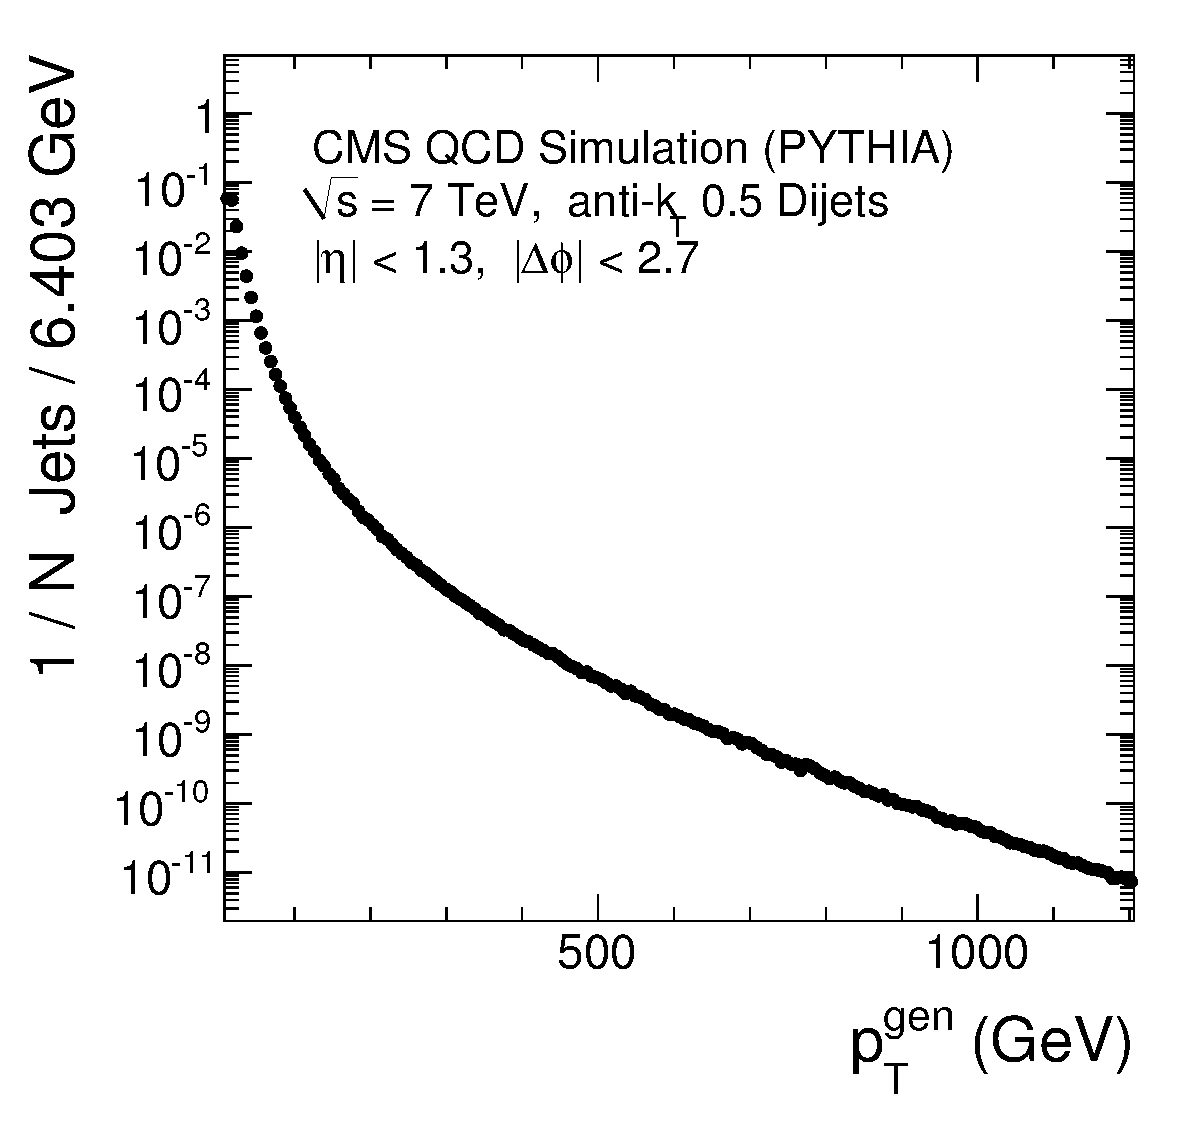
\includegraphics[width=0.45\textwidth]{figures/ExampleSpectrum} &
    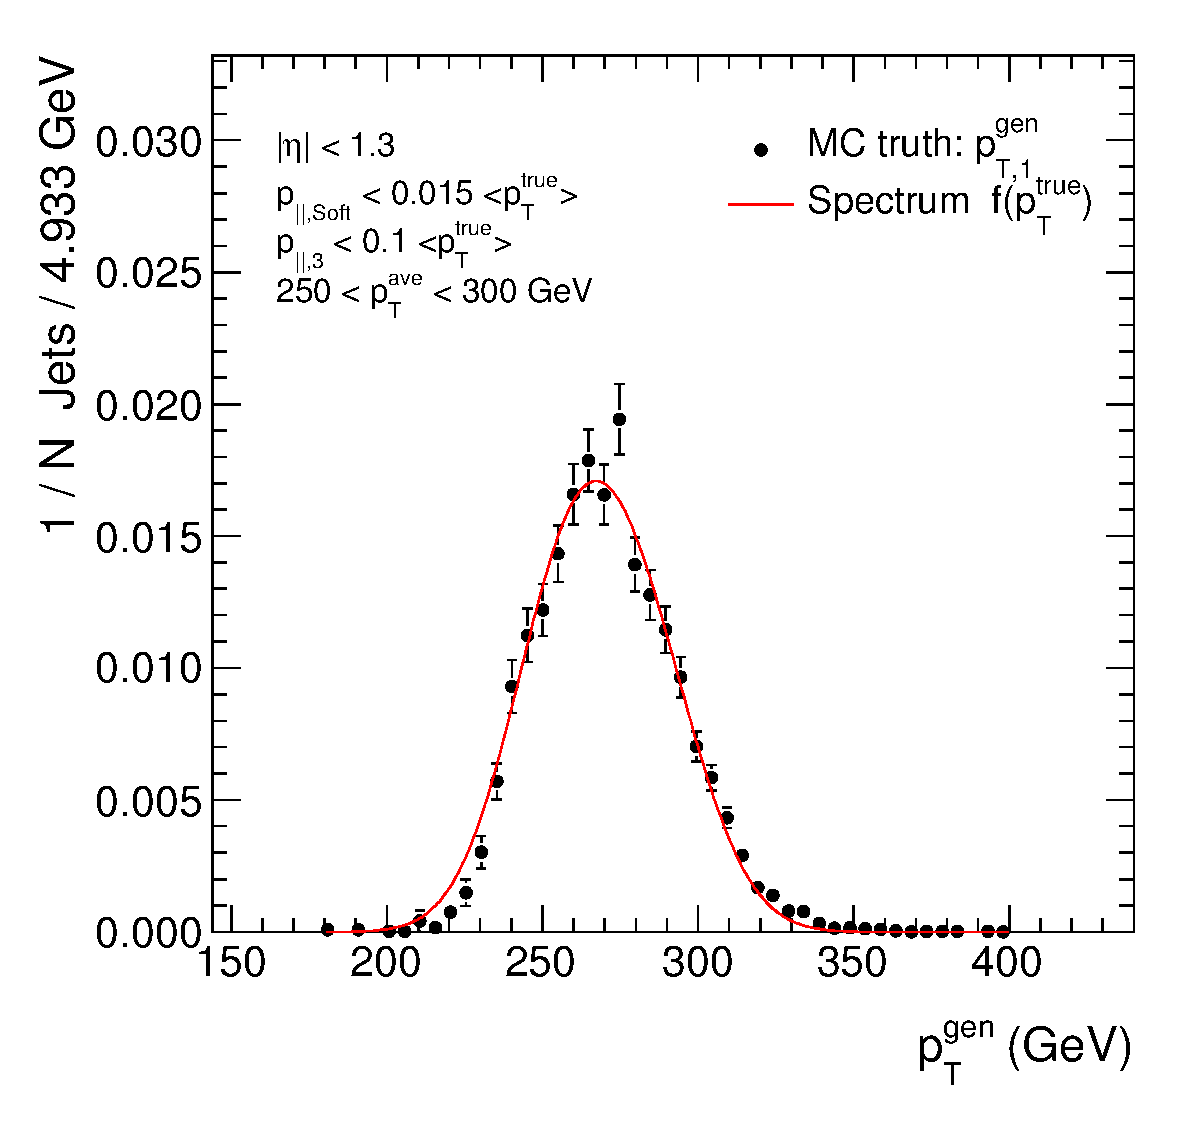
\includegraphics[width=0.45\textwidth]{figures/MaxLike_Eta00-13_SpectrumJet1_PtBin7}\\
 \end{tabular}
  \caption{(\textit{Left}) Dijet \ptgen spectrum from the MC simulation.
    Per selected event, the \ptgen of both the leading jets have been filled into the histogram.
    A linear interpolation of this histogram is used as the particle
    level differential jet cross section~ $f_{0}$ in~\qeq{eq:ResFit:DataDriven:ModifiedSpectrum}.
    (\textit{Right}) \ptgen spectrum (circles) of the selected dijet events in the \mbox{$250 < \ptave < 300\gev$} bin.
    It is well described by the modified cross section $f$ in~\qeq{eq:ResFit:DataDriven:ModifiedSpectrum} (line).}
  \label{fig:ResFit:DataDriven:Spectrum}
\end{figure}

By this extension, additionally a description of biases in the event selection can be included into the likelihood.
Binning in (measured) \ptave causes migration effects at the edges of the selected \ptave range due to the finite jet \pt resolution:
there are jets that fluctuate either into or out of the selected interval.
This is illustrated in \qsubfig{fig:ResFit:DataDriven:Spectrum}{right} with simulated data using the MC truth information.
Additionally, because of the steeply falling dijet \pt spectrum, there are more jets that fluctuate high than jets that fluctuate low in \pt and the selected sample is therefore biased towards jets of lower \ptgen that fluctuated high in the detector.

The dijet pdf~\qeq{eq:ResFit:DijetPdfTransformed} is modified to describe the
\ptave selection and hence avoid biasing the measured resolution.
First, the allowed range of \ptave is considered in the normalisation (comp.~\qeq{eq:ResFit:App:FullPdf} in Appendix~\ref{sec:ResFit:App:Pdf}.)
Second, the \pttrue pdf is extended to incorporate the migration effects:
\begin{equation}
  \label{eq:ResFit:DataDriven:ModifiedSpectrum}
  f\left(\pttrue\right) = \frac{1}{\mathcal{N}_{f}}
  f_{0}\left(\pttrue\right) \int^{\ptavemax}_{\ptavemin}\dif{x}\;\mathcal{G}\left(x|\sigma',\pttrue\right) \, ,
\end{equation}
Here, $f_{0}$ denotes the underlying particle level jet \pt spectrum \qsubfig{fig:ResFit:DataDriven:Spectrum}{left}\footnote{The actual probability densities are evaluated using a linear interpolation of the histogram.} and $\mathcal{G}$ is a Gaussian of width \mbox{$\sigma' = \sigma/\sqrt{2}$}, \ie the pdf of \ptave for a given \pttrue.
Equation~\qeq{eq:ResFit:DataDriven:ModifiedSpectrum} is validated using simulate data:
the \ptgen spectrum of selected dijet events is well described by $f(\pttrue)$ as demonstrated in \qsubfig{fig:ResFit:DataDriven:Spectrum}{right}.
This extension to $f$ depends solely on the fitted parameter $\sigma'$ and does not introduce any new dependencies on the MC simulation.



\subsection{Influence of Additional Hadronic Activity and Hadronisation Effects}\label{sec:ResFit:DataDriven:AddJets}

\subsubsection{Contributions to the Dijet Asymmetry}\label{sec:ResFit:DataDriven:AddJets:Contributions}

In \qsubfig{fig:ResFit:DataDriven:AddJets:Bias}{right}, the standard deviations of
the asymmetry distribution, multiplied by a factor $\sqrt{2}$,
are shown for various \ptgen bins for simulated dijets.
According to~\qeq{eq:ResFit:ResFromAsym} these should correspond to the
jet \pt resolution.
However, they are greater than the MC truth resolutions\footnote{The
  determination of the MC truth resolution is discussed in
  Appendix~\ref{sec:ResFit:App:MCTruth}.} $\sigma(R_{\text{MC}})$ for
the following reasons:
The dijet asymmetry~\qeq{eq:ResFit:Asymmetry} is defined under the assumption of exactly two jets which are balanced in transverse momentum at particle level.
Additional jet activity in the events, \eg from soft gluon
radiation, causes an imbalance of the leading two jets and hence
broadens the measured asymmetry distribution.

\begin{figure}[ht]
 \centering
  \begin{tabular}{cc}
    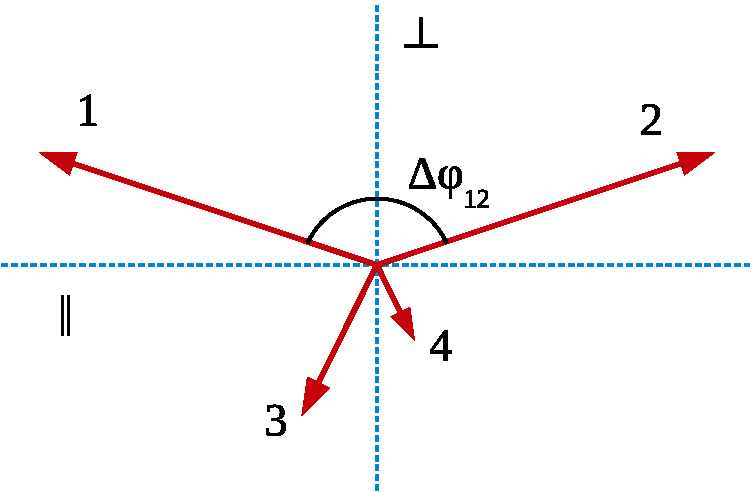
\includegraphics[width=0.45\textwidth]{figures/Sketch_Projections} &
    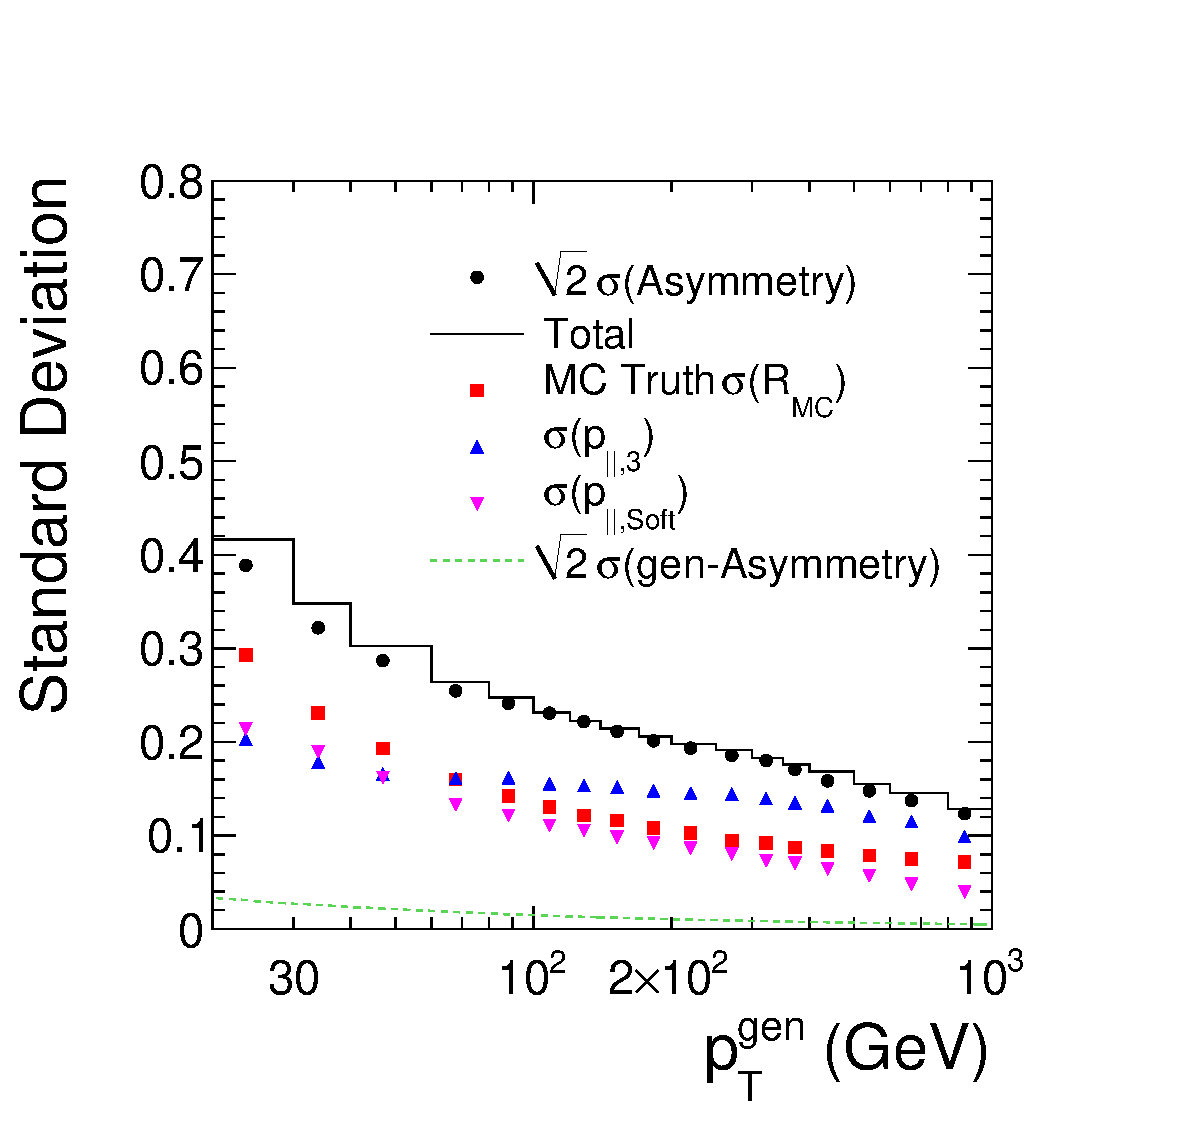
\includegraphics[width=0.45\textwidth]{figures/Spring10QCDDiJet_ParallelComponent_hParallelContributions} \\
 \end{tabular}
  \caption{(\textit{Left}) Definition of the dijet axis $\phi_{||}$, the direction normal to the
    angle bisector of the leading two jets in the transverse plane.
    Additional jets with \pt components along $\phi_{||}$ will cause
    a \pt imbalance of the particle jets and bias the measured
    resolution towards greater values. 
    (\textit{Right}) Demonstration of the different
    contributions biasing the measured dijet asymmetry and hence resolution.
    Shown are the standard deviations of the distributions of the
    different quantities described in the text. 
    Their quadratic sum (solid line) is in fair agreement to the
    measured asymmetry (solid circles).
    For this plot, simulated dijet events have been preselected by requiring \mbox{$|\Delta\phi_{12}| > 2.7$}.
 }
  \label{fig:ResFit:DataDriven:AddJets:Bias}
\end{figure}

As illustrated in \qsubfig{fig:ResFit:DataDriven:AddJets:Bias}{left}, not the
absolute \pt of the additional jets actually affects the balance, but rather the component along the dijet axis, $\phi_{||}$, defined as the direction normal to the angle bisector of the leading two jets.
The \pt components parallel to $\phi_{||}$ of the third and all further
(\textit{soft}) jets may be defined as
\begin{align}
  \begin{split}
    \ppi{3}               & =  |\pti{3}\cos(\phi_{3}-\phi_{||})| \\
    \ppi{\text{Soft}} & =  |\sum_{i>3}\pti{i}\cos(\phi_{i}-\phi_{||})| \,.
  \end{split}
\end{align}
The total standard deviation of the measured dijet asymmetry
distribution (multiplied by $\sqrt{2}$) can hence be understood as the
quadratic sum of the underlying dijet asymmetry due to the jet \pt response,
$\sigma(R_{\text{MC}})$, and the standard deviations of the \pp
distributions, $\sigma(\ppi{3})$ and
$\sigma(\ppi{\text{Soft}})$,
\begin{equation}
  \label{eq:ResFit:TotalAsym}
  \text{Total} = \sigma(R_{\text{MC}}) \oplus \sigma(\ppi{3}) \oplus
  \sigma(\ppi{\text{Soft}}) \oplus \sqrt{2}\cdot\sigma(A^{\text{gen}}) \,.
\end{equation}

The transverse momentum balance assumed for the particle level jets
actually takes place at parton level.
Owing to the statistical nature of the fragmentation and hadronisation
process, fluctuations in the
fraction of energy of the original partons clustered into jets are
expected (\textit{out-of-cone}).
This is an additional mechanism introducing an imbalance in the
dijet events and the contribution is estimated using the \ptgen
asymmetry, $A^{\text{gen}}$, in perfect
two jet events.
The standard deviation $\sqrt{2}\cdot\sigma(A^{\text{gen}})$ is also added in quadrature to
$\sigma(R_{\text{MC}})$, hence the last term in~\qeq{eq:ResFit:TotalAsym}.

The dijet pdf~\qeq{eq:ResFit:DijetPdf} has been shown to be a pdf of
the dijet asymmetry and has also been defined under the assumption of \pt
balance at particle level.
Hence it will be biased by the same effects.



\subsubsection{Correction for Additional Hadronic Activity}\label{sec:ResFit:DataDriven:AddJets:Extrapolation}

In order to compensate for the presence of additional jets,
events are selected\footnote{The resulting selection bias is incorporated in the dijet pdf as
before, comp. \qsec{sec:ResFit:DataDriven:FullFit}.} in reasonably small bins of \ptave.
Per bin, the \pp components of the third and all further jets are restricted to
\begin{align}
  \label{eq:ResFit:ThirdJetSelection}
  \begin{split}
    \ppi{3}                & < z\cdot\mean{\pttrue} \\
    \ppi{\text{Soft}}  & < 0.015\cdot\mean{\pttrue},
 \end{split}
\end{align}
where $\mean{\pttrue}$ is the mean particle level jet \pt in that bin
as estimated from the assumed spectrum
$f$ in~\qeq{eq:ResFit:DataDriven:ModifiedSpectrum}.
Several sets of dijet events are selected, each with a different
threshold $z$ of \ppi{3}, and the mean Gaussian response with \pt
independent resolution $\sigma$ is measured by maximising the dijet
likelihood~\qeq{eq:ResFit:Likelihood} w.r.t. $\sigma$.
The dependence of the jet \pt resolution on the threshold $z$ is
clearly visible in \qfig{fig:ResFit:DataDriven:AddJets:Corr}.
In order to extrapolate the measurement to the case of a two jet only
event, the \mbox{$\sigma/\mean{\pttrue}$} are fitted with a linear
function and the $y$ axis intercept is used as the unbiased jet \pt
resolution.

\begin{figure}[ht]
 \centering
 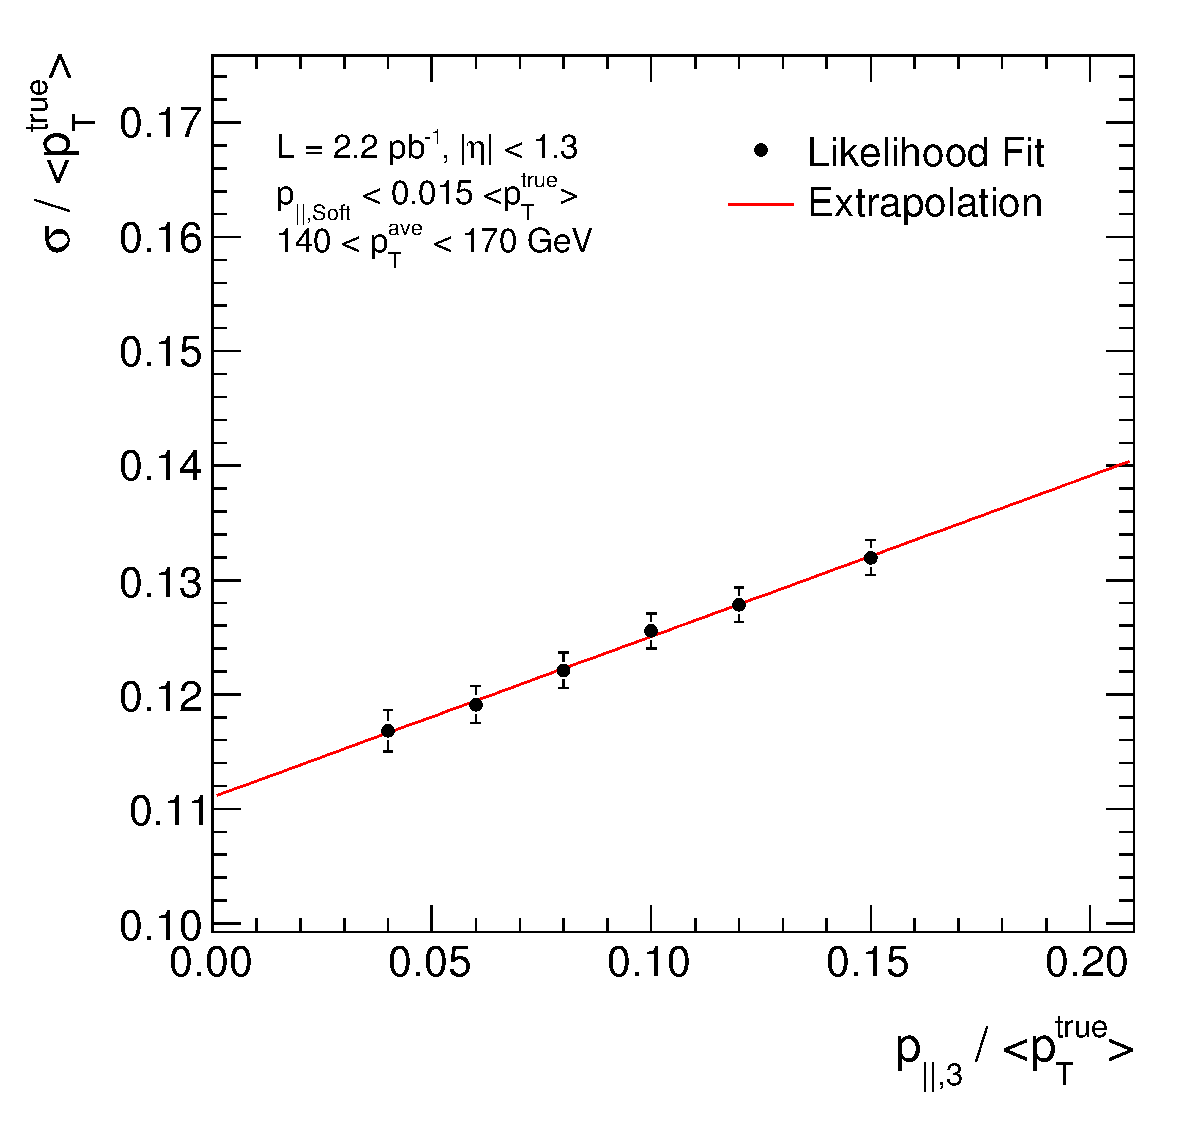
\includegraphics[width=0.45\textwidth]{figures/MaxLike_Data132440-144011_Eta00-13_ExtrapolatedPar0_PtBin4}
 \caption{(\textit{Right}) Gaussian resolutions \mbox{$\sigma/\mean{\pttrue}$} measured with the unbinned
    fit in Collider data for \mbox{$140 < \ptave < 170\gev$} and different \ppi{3}
    thresholds after suppression of additional soft jet activity along
    $\phi_{||}$. 
    \mbox{$\sigma/\mean{\pttrue}$} of \ppi{3} is linearly
    extrapolated to the case of an ideal dijet event.
  }
  \label{fig:ResFit:DataDriven:AddJets:Corr}
\end{figure}

In the following, the statistical uncertainty on the fitted $y$ axis
intercept is used as statistical uncertainty of the measured resolution.
Due to the selection requirement~\qeq{eq:ResFit:ThirdJetSelection},
all events selected for a particular value of the threshold $z$ are
also included in the samples selected with larger values of $z$.
Hence, the measured resolutions in one \ptave bin are strongly correlated.
This correlation is not considered in the quoted uncertainties yet.

The contribution due to out-of-cone effects to the bias is small, of
the order of $1\%$, as shown in
\qsubfig{fig:ResFit:DataDriven:AddJets:Bias}{right}.
Hence, this bias is corrected for using the MC simulation:
The width of the \ptgen asymmetry, $\sigma(A^{\text{gen}})$, is determined for the
 case of perfectly balanced dijet events, using the
same extrapolation technique as above.
The extrapolated jet \pt resolution is then corrected by 
subtracting $\sqrt{2}\cdot\sigma(A^{\text{gen}})$ in quadrature.

The need for compensating the influence of additional jet activity is
the reason why a mean, \pt independent Gaussian the resolution is
measured per \ptave bin.
In that case there is only one free parameter, $\sigma$, which can be
extrapolated in a straight forward way.
Was the response instead parameterised with a \pt dependent function,
\eg a Gaussian with width \mbox{$\sigma(\pt) = a\pt \oplus
  b\sqrt{\pt} \oplus c$},
the parameters $a$, $b$, and $c$ are correlated.
In that case it is not clear how the extrapolation should be
performed.
The method of the maximum likelihood fit itself is not affected by the
parameter correlation, however, and can very well measure the
parameters of a \pt dependent resolution $\sigma(\pt)$ as demonstrated
in Appendix~\ref{sec:ResFit:App:ToyMC} using a toy MC simulation.


\section{Systematic Uncertainties}\label{sec:ResFit:Systematics}

Sources of systematic uncertainties are
\begin{itemize}
\item Form of spectrum taken from MC simulation
\item Assumption of JES of one (corresponds to shift of spectrum)
\item Extrapolation procedure i.e. integrated bins and linear extrapolation  
\end{itemize}
\section{Results}

The measured Gaussian resolutions, corrected for the effects of
additional jets and out-of-cone showering, are shown for different
\ptref in \qsubfig{fig:ResFit:ResoGauss}{left} for simulated
data.
Here, the \ptref are the mean values of the asssumed spectra~$f(\pttrue)$
in each \ptave bin (comp. \qsubfig{fig:ResFit:Asym:Spectrum}{right}).
The error bars represent the statistical uncertainty from the
extrapolation procedure only (comp. the corresponding remarks in
\qsec{sec:ResFit:AddJets:Extrapolation}).
The measured resolutions are compared to the MC truth resolution.
The latter has been derived from Gaussian fits to the bulk of the
\mbox{$\pt / \ptgen$} distributions of the leading two generator
level jets in an event in small bins of \ptgen, where the
detector level jets are required to match the generator level jets
within a distance of $0.2$ in \mbox{$(\eta,\phi)$} space.
There is good closure of the presented method.

The corresponding measurement in Collider data is shown in \qsubfig{fig:ResFit:ResoGauss}{right}.
The jet \pt resolution is underestimated by about $10\%$ in the MC simulation.

\begin{figure}[ht]
  \label{fig:ResFit:ResoGauss}
  \centering
  \begin{tabular}{cc}
    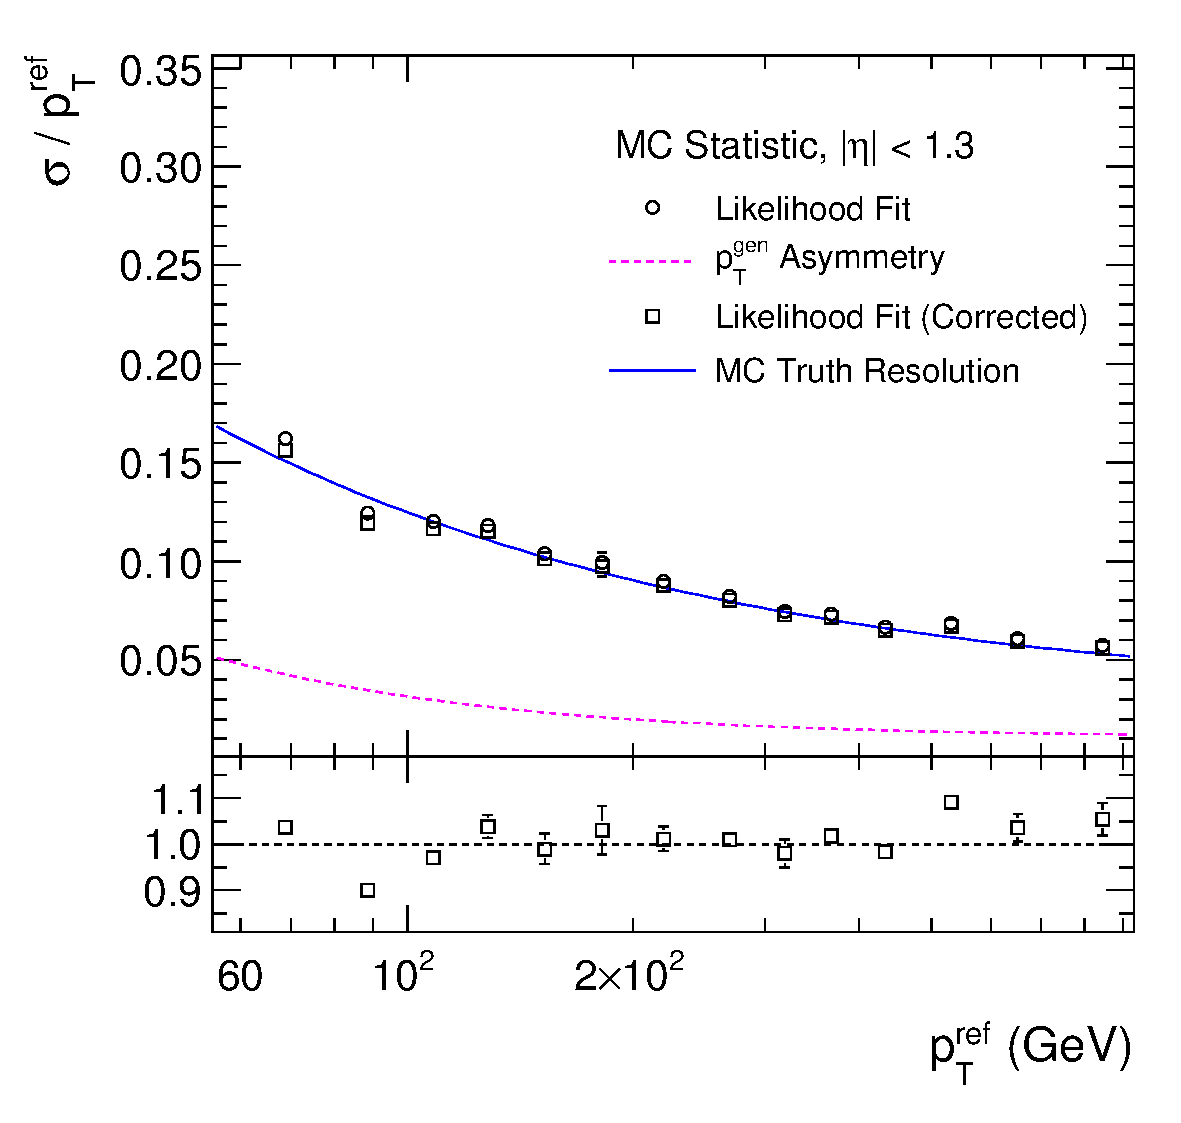
\includegraphics[width=0.45\textwidth]{figures/MaxLike_Eta00-13_ExtraResoBottomRatio}
    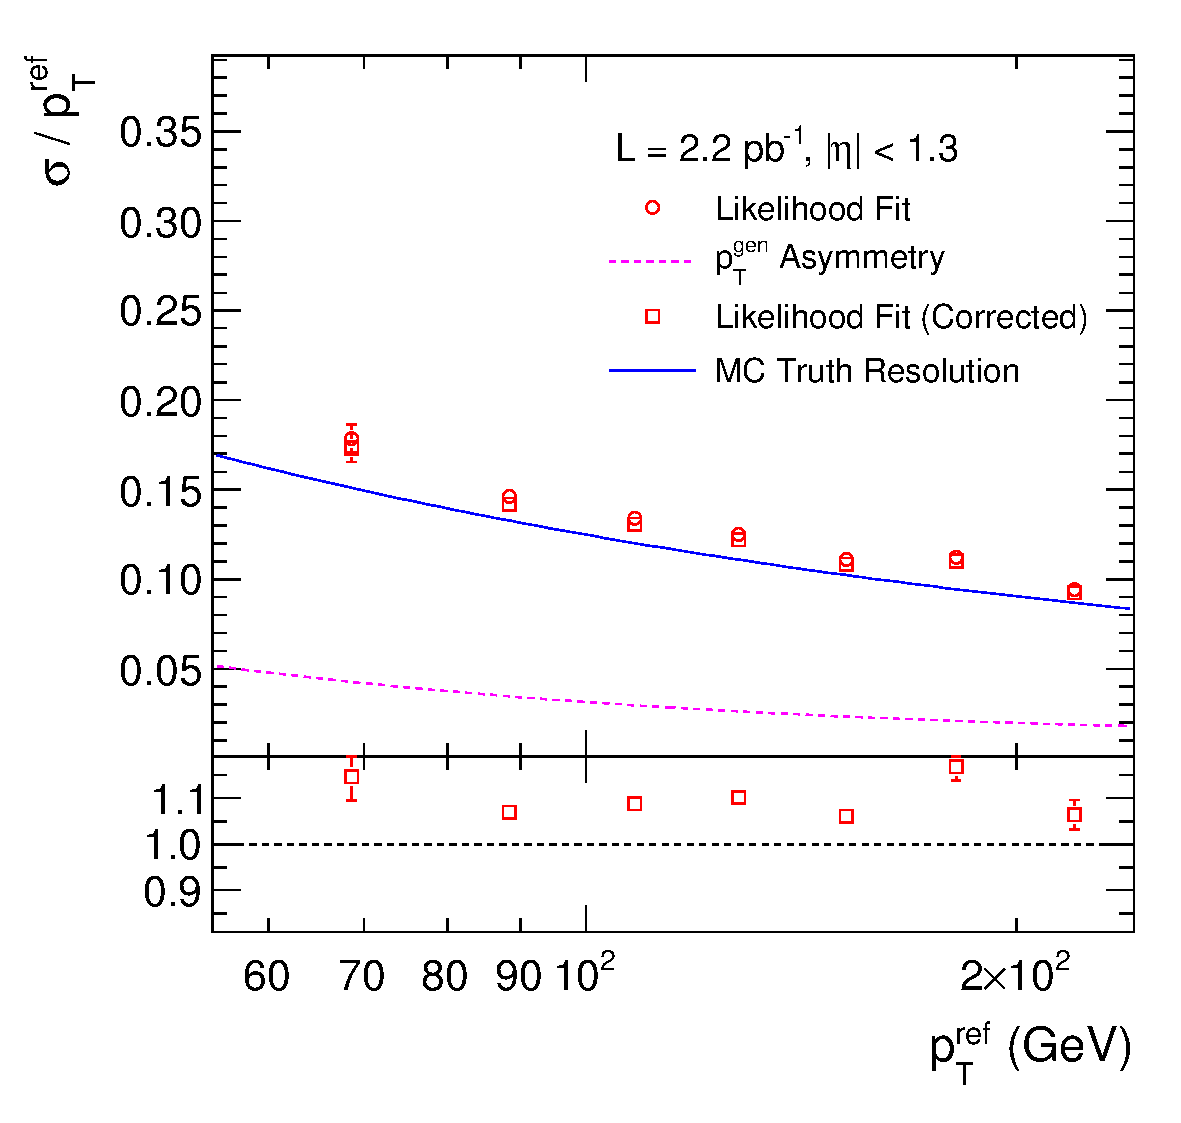
\includegraphics[width=0.45\textwidth]{figures/MaxLike_Data132440-144011_Eta00-13_ExtraResoBottomRatio}\\
  \end{tabular}
  \caption{Measured Gaussian resolutions corrected for
    contributions from additional jets (circles) in different \pt bins.
    Out-of-cone contributions (dashed line) are substracted in
    quadrature to obtain the final resolution (squares).
    The \ptref are the mean values of the asssumed spectra~$f(\pttrue)$
    in each bin (comp. Fig.~\ref{fig:qcd:resolMaxlike:ptGenSpectra}
    (right)).
    (\textit{Left}) Measured resolution in simulated data; there is good
    agreement to the MC truth resolutioin (solid line).
    (\textit{Right}) Measured resolution in Collider data; it is
    $\approx10\%$ larger than the simulation.
  }
\end{figure}

\appendix


\section{Gaussian resolution from Monte Carlo truth information}\label{sec:ResFit:QCDMC:MCTruthReso}

The jet \pt resolution is determined from Monte Carlo truth information, first, as a reference to compare the measured resolution to, and second, as an input $r_{0}$ in~\eqref{eq:ResFit:Method:ModifiedSpectrum} to incorporate the the selection bias into the dijet likelihood (comp. Section~\ref{sec:ResFit:Method:Biases}).
\begin{figure}[ht]
  \centering
  \begin{tabular}{cc}
    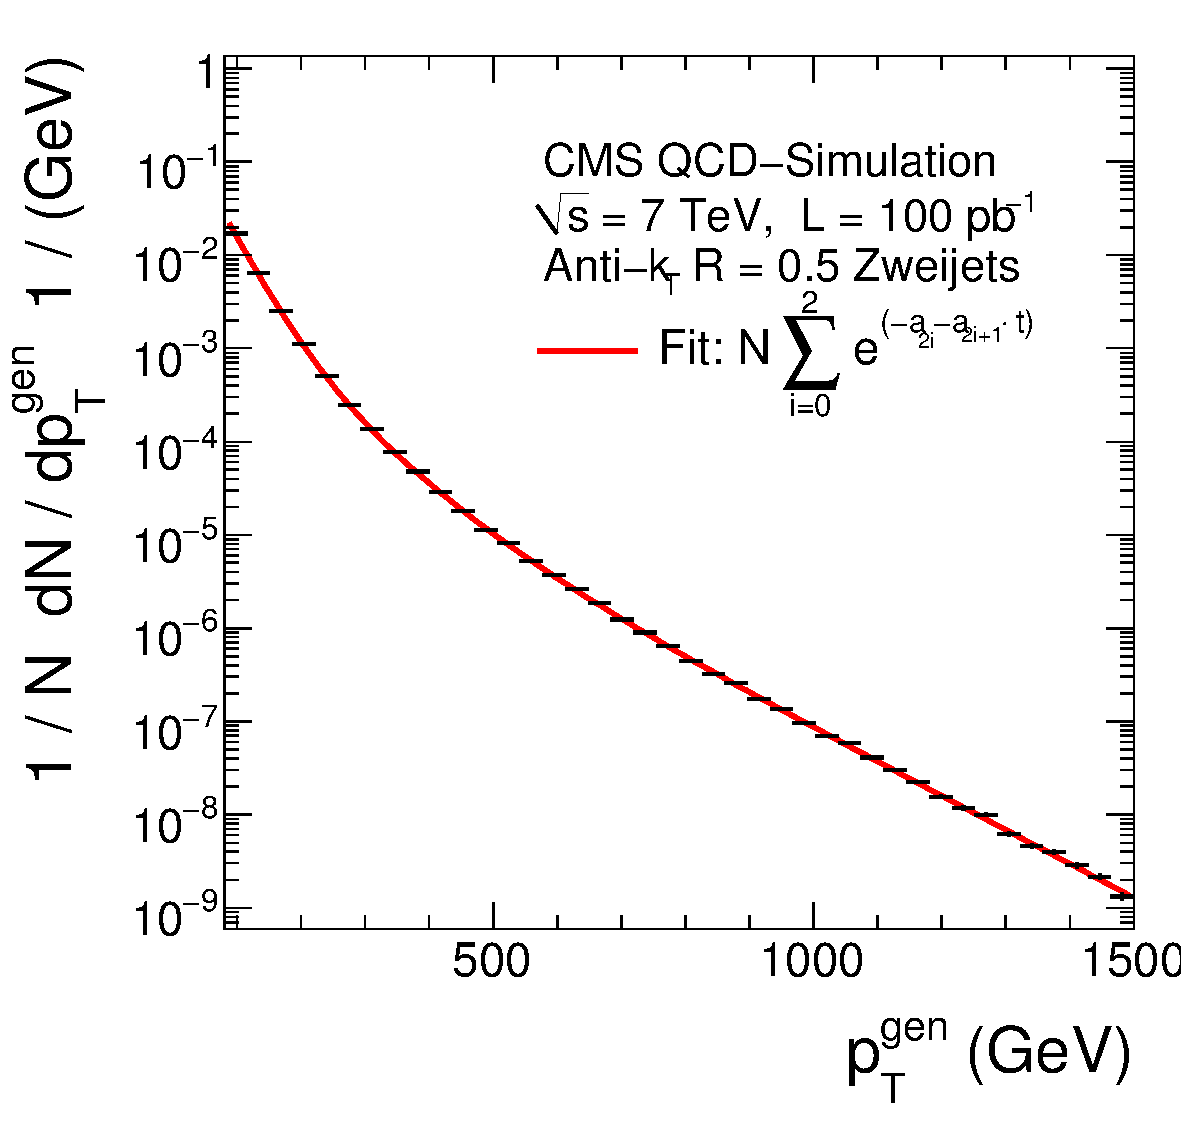
\includegraphics[width=0.45\textwidth]{figures/resFit_QCD_MCSpectrum}
    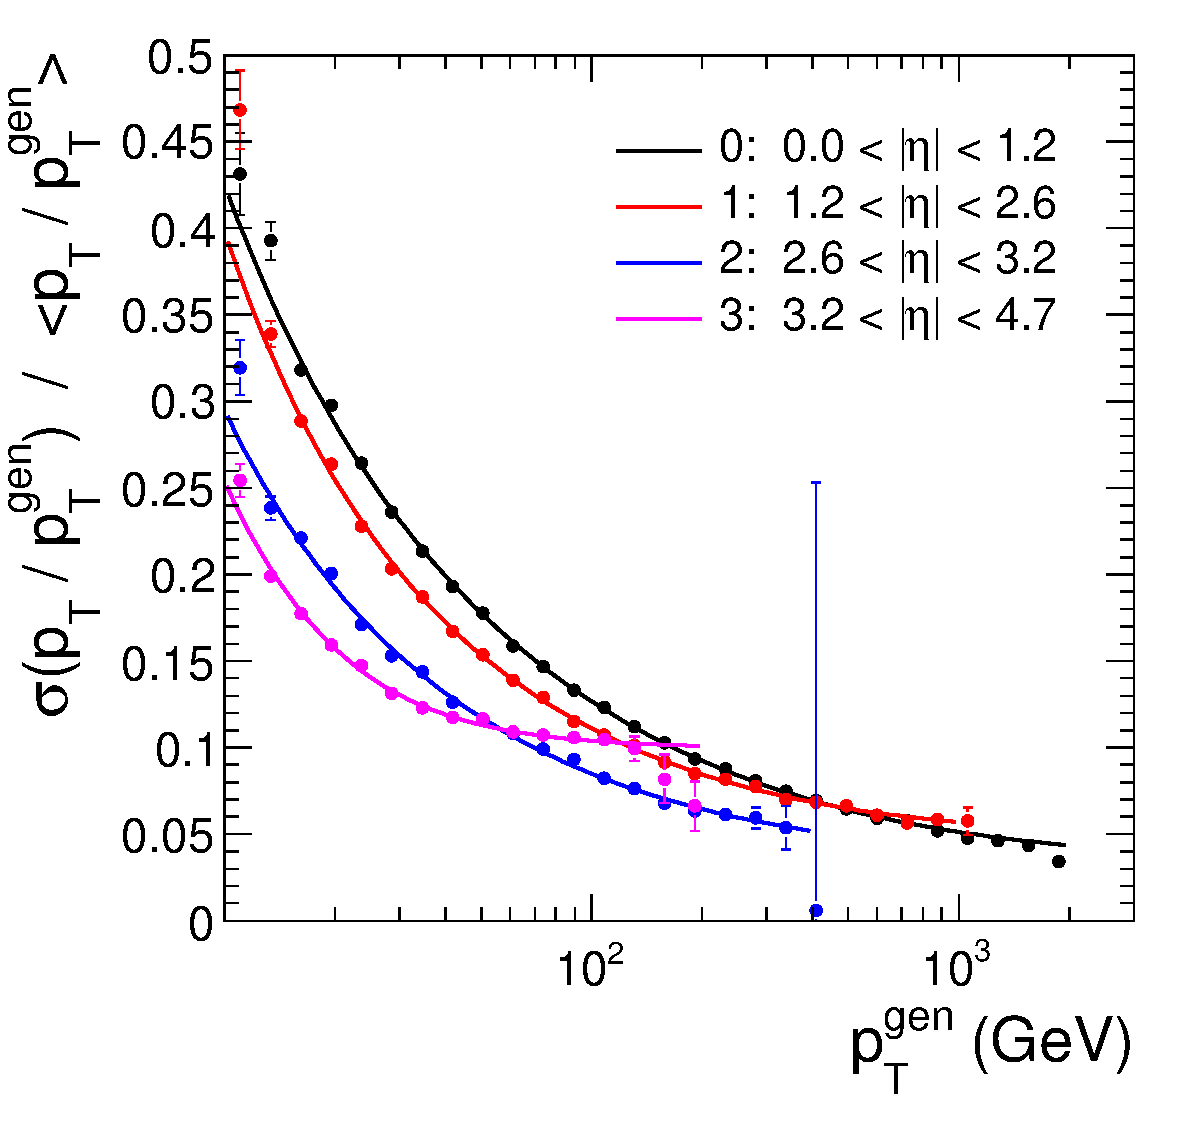
\includegraphics[width=0.45\textwidth]{figures/resFit_QCD_MCTruthResolution}
  \end{tabular}
  \caption{(\textit{Left}) QCD dijet \ptgen spectrum. (\textit{Right}) Relative Gaussian jet \pt resolution $\sigma/\pt$ derived from Monte Carlo truth as a function of \pt in different $\eta$ bins.}
  \label{fig:ResFit:QCDMC:MCTruthReso}
\end{figure}
The determination follows closely~\cite{bib:cmsan:mcjer}:
In each event, the two jets with highest particle level jet \pt, \ptgen, are selected and the response distributions \mbox{$\pt / \ptgen$} are recorded in different bins of \ptgen and $\eta$ (the $\eta$ binning is listed in Table~\ref{tab:ResFit:QCDMC:MCTruthReso}).

--- Define matching ??? ---

The central part of each distribution --- defined by the interval of 1.5 standard deviations around the mean --- is fitted with a Gaussian.
In each $\eta$ bin, the fitted Gaussian widths $\sigma$ are interpolated for different \pt by the usual parametrisation function~\eqref{eq:ResFit:ToyMC:Sigma}.
The fitted Gaussian widths and the interpolation functions are shown in Fig.~\ref{fig:ResFit:QCDMC:MCTruthReso}; the corresponding parameter values are listed in Table~\ref{tab:ResFit:QCDMC:MCTruthReso}.
\begin{table}[ht]
  \caption{Parameters of the MC truth resolution $\sigma$.}
  \centering
  \begin{tabular}[h]{cccccc}
    \toprule
    & $|\eta_{\text{min}}|$ & $|\eta_{\text{max}}|$ & $\xi_{0}\,(\text{Ge}\kern-0.06667em\text{V})$ & $\xi_{1}\,(\sqrt{\text{Ge}\kern-0.06667em\text{V}})$ & $\xi_{2}$ \\
    \midrule
    $0$ & $0$ & $1.2$ & $1.9\pm0.2$ & $1.205\pm0.006$  & $0.0342\pm0.0007$ \\
    $1$ & $1.2$ & $2.6$ & $2.51\pm0.09$ & $0.968\pm0.009$  & $0.0483\pm0.0009$ \\
    $2$ & $2.6$ & $3.2$ & $1.7\pm0.18$ & $0.76\pm0.02$  & $0.035\pm0.004$ \\
    $3$ & $3.2$ & $4.7$ & $2.2\pm0.1$ & $0.2\pm0.1$  & $0.099\pm0.003$ \\
    \bottomrule
  \end{tabular}
  \label{tab:ResFit:QCDMC:MCTruthReso}
\end{table}


\section{Study with a Toy Monte Carlo Simulation}\label{sec:ResFit:App:ToyMC}

\fixme{Shorter}

The method presented in the previous Section~\ref{sec:ResFit:App:Method}
is studied using a simple simulation, \textit{Toy Monte Carlo}.
First, the basic likelihood fit described in
Section~\ref{sec:ResFit:App:Method:Likelihood} is performed (Section~\ref{sec:ResFit:App:ToyMC:PtGenCuts}),
whereby events have been selected using Monte Carlo truth information.
Second, a data driven event selection has been applied and the
modified likelihood, described in
Section~\ref{sec:ResFit:App:Method:Biases}, is maximised (Section~\ref{sec:ResFit:App:ToyMC:PtCaloCuts}).


\subsection{Generated sample}\label{sec:ResFit:App:ToyMC:Sample}

A sample of $30\,000$ ideal dijet events has been generated assuming a
simple exponential particle level jet \pt spectrum
\begin{equation}
  \label{eq:ResFit:ToyMC:Spectrum}
  f\left(\pttrue\right) \propto \exp\left(-\pttrue / \tau\right),
  \qquad \tau = 80.
\end{equation}
ranging from \mbox{$50 < \pttrue < 1000\gev$} (comp. Fig.~\ref{fig:ResFit:App:ToyMC:Sample:Spectrum}).
Two independent measurements of the jet \pt have been simulated by
weighting \pttrue with random numbers drawn from a Gaussian response
\begin{equation}
  \label{eq:ResFit:ToyMC:Response}
  r_{\mathbf{\xi}}\left(\pt|\pttrue\right) = 
  \frac{1}{\sqrt{2\pi}\sigma}\exp\left[-\frac{1}{2}\left(\frac{\pt - \pttrue}{\sigma}\right)^{2}\right]
\end{equation}
(Here and in the following the jet index $i$ has been omitted.)
The standard deviation, i.e. the jet resolution, $\sigma$ has been parametrised as a function of \pttrue and
the parameters $\xi_{i}$, \mbox{$i\in [0,2]$}, as
\begin{equation}
  \label{eq:ResFit:ToyMC:Sigma}
  \sigma = \xi_{0}\gev
  \oplus \xi_{1}\,\sqrt{\pt\gev}\oplus \xi_{2}\pt.
\end{equation}
The values of the parameters $\mathbf{\xi}$ are listed in
Tab.~\ref{tab:ResFit:ToyMC:PtGenCuts:FitResult}.
An example of a simulated response distribution is shown in Fig. ~\ref{fig:ResFit:App:ToyMC:PtGenCuts:Response}.

\begin{figure}[ht]
  \centering
  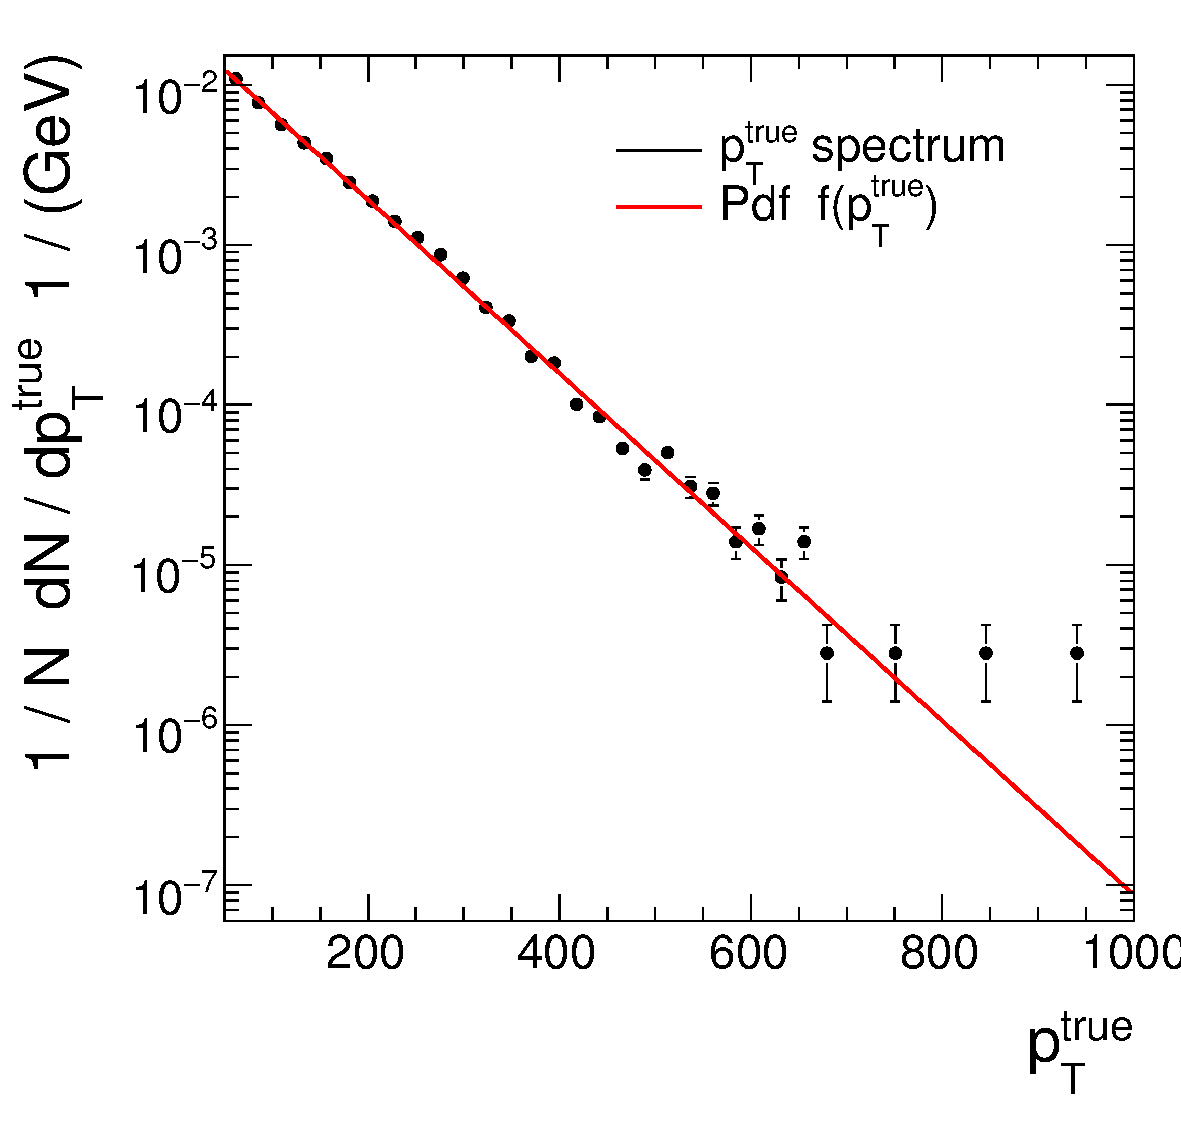
\includegraphics[width=0.45\textwidth]{figures/resFit_ToyMC_PtGenCuts_SpectrumLog}
  \caption{Toy Monte Carlo simulation of a sample of ideal dijet events.
    Generated \pttrue spectrum (circular markers) and the underlying pdf (solid line).}
  \label{fig:ResFit:App:ToyMC:Sample:Spectrum}
\end{figure}


\subsection{Measurement of the resolution with a truth information based event selection}\label{sec:ResFit:App:ToyMC:PtGenCuts}

The jet energy resolution of the dijet sample is to be measured as described in Section~\ref{sec:ResFit:Method:Likelihood}.
Dijet events are have been selected from the sample described above by
requiring \mbox{$\ptmin < \pttrue < \ptmax$}.
The jet \pt spectrum is taken directly from the
simulation~\eqref{eq:ResFit:ToyMC:Spectrum}, while the jet \pt
response is assumed to be Gaussian and the resolution $\sigma$ to
depend on \pttrue and the parameters $\mathbf{\xi}$ as
in~\eqref{eq:ResFit:ToyMC:Sigma}.

\begin{figure}[ht]
\centering
\begin{tabular}{cc}
  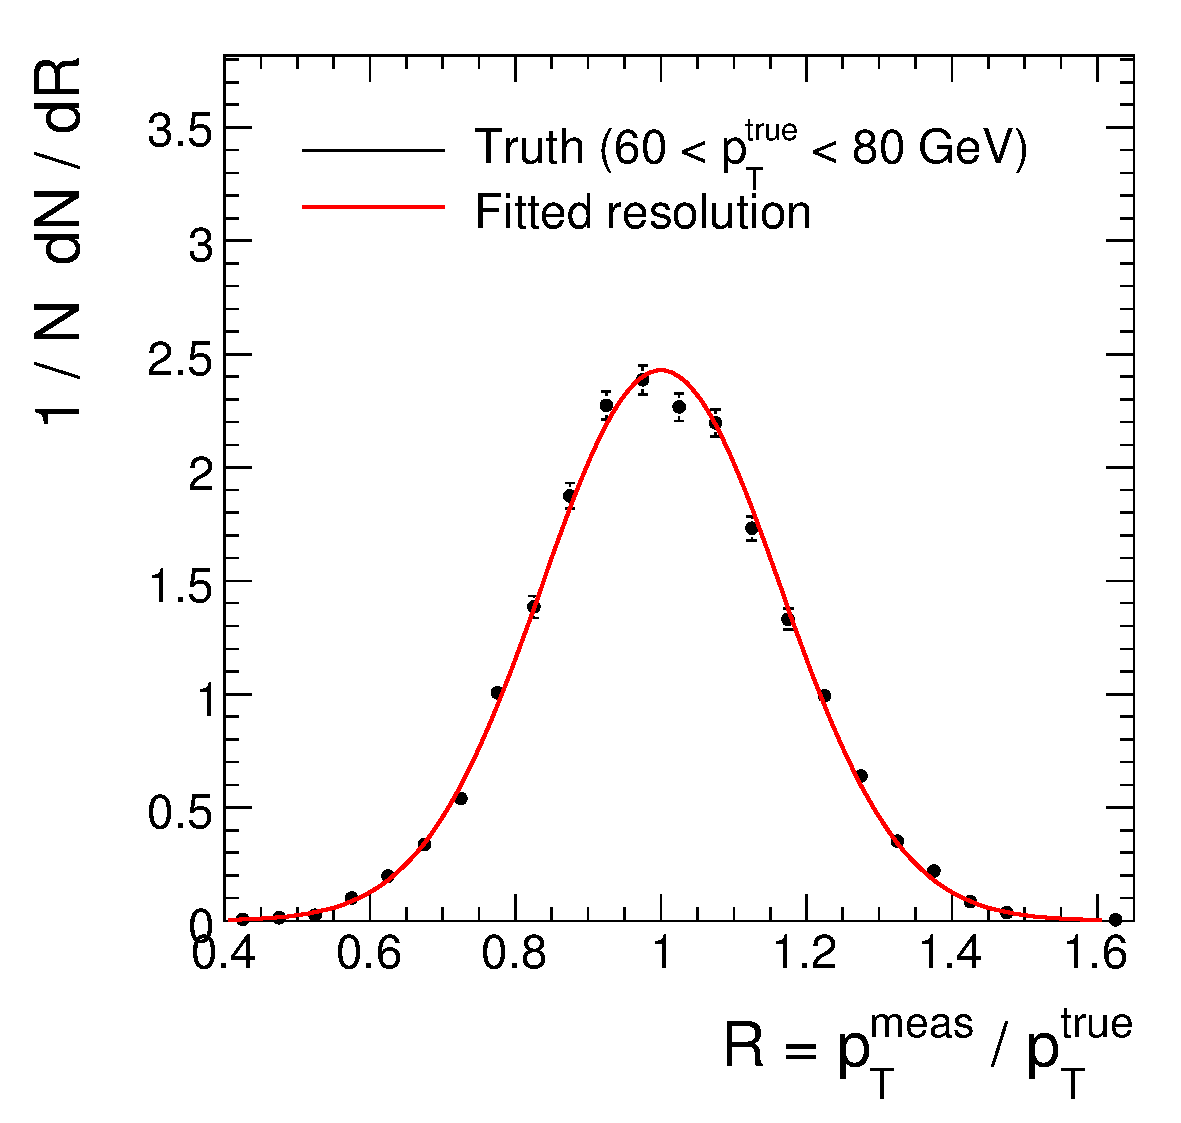
\includegraphics[width=0.45\textwidth]{figures/resFit_ToyMC_PtGenCuts_ResolutionBin1} &
  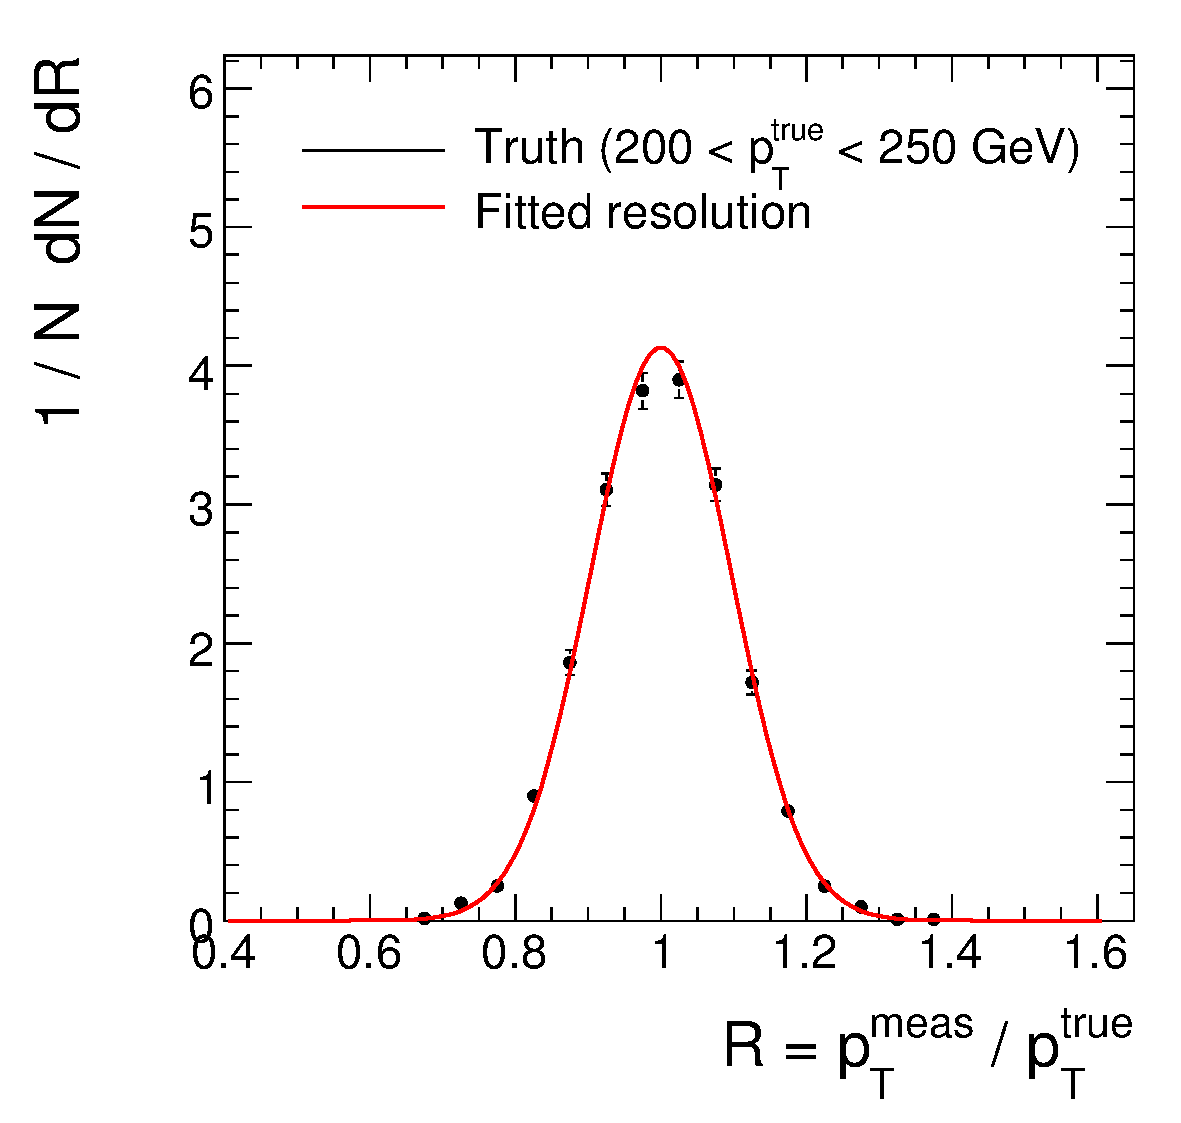
\includegraphics[width=0.45\textwidth]{figures/resFit_ToyMC_PtGenCuts_ResolutionBin7} \\      
\end{tabular}
\caption{Simple simulation of a sample of ideal dijet events.
  Generated true response \mbox{$\pt / \pttrue$} (histogram) and
  the response (solid line) from the maximum likelihood fit in two
  different \pttrue bins.
  The latter has been evaluated for the mean \pttrue in these bins.
  Note, here ``fit'' does not refer to a fit to the shown histogram but the maximisation of the likelihood~\eqref{eq:ResFit:Likelihood}.
}
\label{fig:ResFit:App:ToyMC:PtGenCuts:Response}
\end{figure}


\begin{table}[ht]
  \caption{Parameter values of the Gaussian jet \pt resolution
    $\sigma$.
    Listed are the true values used for the generation and
    the fitted values.
    The uncertainties assigned to the fitted values
    are the statistical uncertainties from the fit.
    The parameter correlations are shown in Fig.~\ref{fig:ResFit:App:ToyMC:PtGenCuts:ParCorr}.}
  \centering
  \begin{tabular}[ht]{lccc}
    \toprule
    $\xi_{i}$ & $0$ & $1$ & $2$ \\
    \midrule
    True value & $4$           & $1.2$           & $0.05$ \\
    Fit result & $4.5 \pm 0.7$ & $1.18 \pm 0.05$ & $0.051 \pm 0.004$ \\
    \bottomrule
  \end{tabular}
  \label{tab:ResFit:ToyMC:PtGenCuts:FitResult}
\end{table}


\begin{figure}[ht]
  \centering
  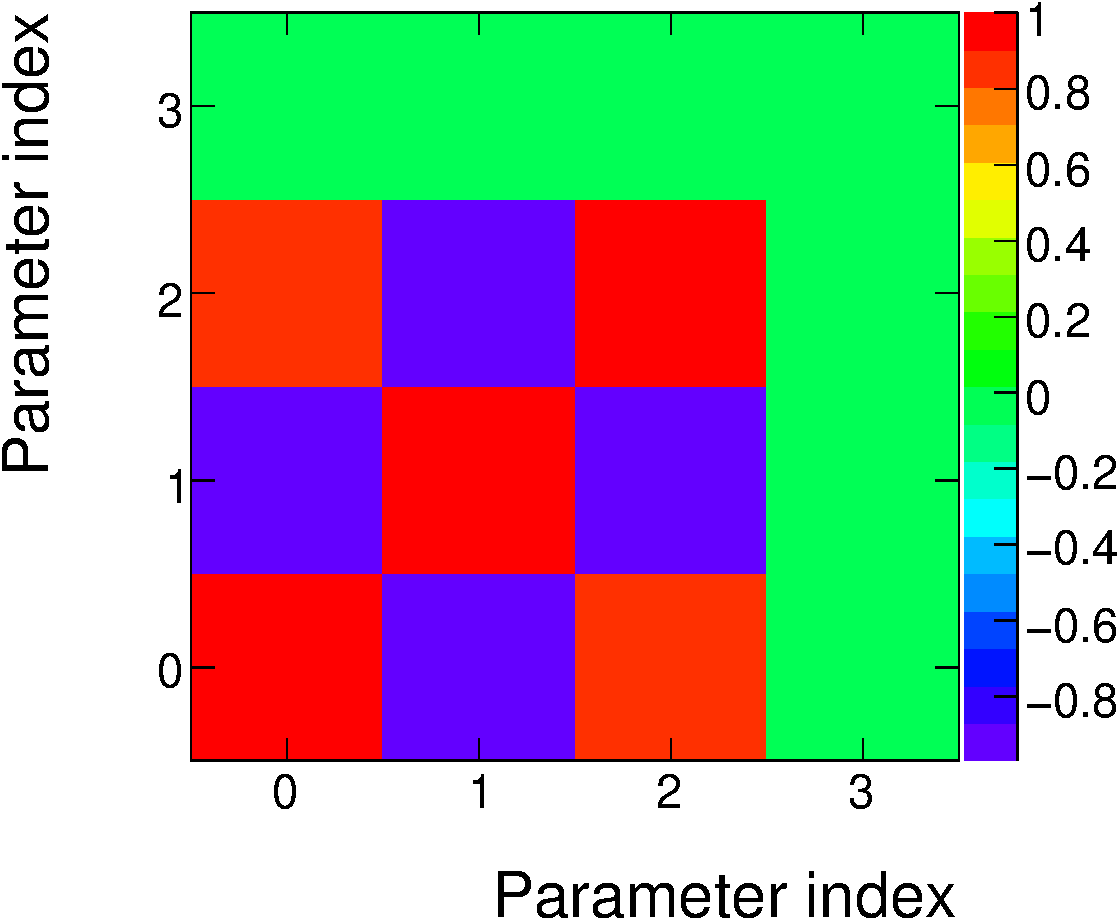
\includegraphics[width=0.45\textwidth]{figures/resFit_ToyMC_PtGenCuts_Correlations}
  \caption{Correlation coefficients of the fitted parameter values
    $\mathbf{\xi}$ of the Gaussian jet \pt resolution $\sigma$. 
    Parameter $3$ corresponds to the slope $\tau$ of the
    spectrum, which is fixed during the fit, and is to be ignored.}
  \label{fig:ResFit:App:ToyMC:PtGenCuts:ParCorr}
\end{figure}

The fitted parameter values $\mathbf{\xi}$ are listed in Tab.~\ref{tab:ResFit:ToyMC:PtGenCuts:FitResult};
they agree with the true values within the statistical uncertainties.

The parameters are strongly (anti-) correlated (comp. Fig.~\ref{fig:ResFit:App:ToyMC:PtGenCuts:ParCorr}).
In the present \pttrue interval from \mbox{$\ptmin = 50\gev$} to \mbox{$\ptmax = 1000\gev$}, the used parametrisation of the Gaussian resolution $\sigma$ is over-determined.
The $\xi_{0}$ term in~\eqref{eq:ResFit:ToyMC:Sigma} is most important at very low \pt while the $\xi_{2}$ term dominates at very large \pt.
Hence, omitting either the terms with $\xi_{0}$ and $\xi_{2}$ or the
term with $\xi_{1}$ would have been sufficient to describe the measured events.

\begin{figure}[ht]
  \centering
  \begin{tabular}{cc}
    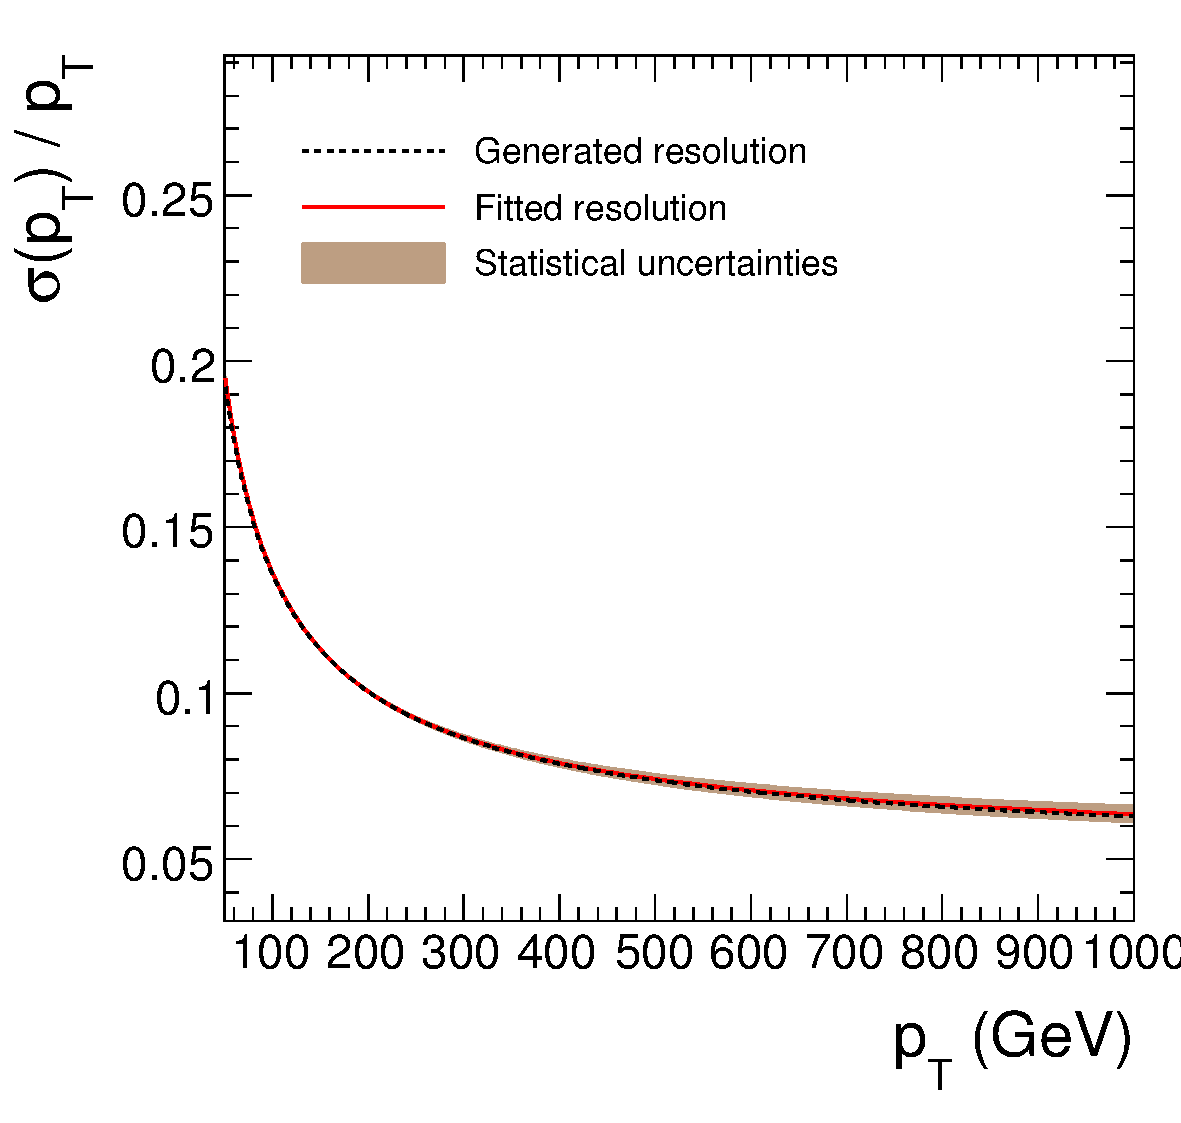
\includegraphics[width=0.45\textwidth]{figures/resFit_ToyMC_PtGenCuts_Sigma} &
    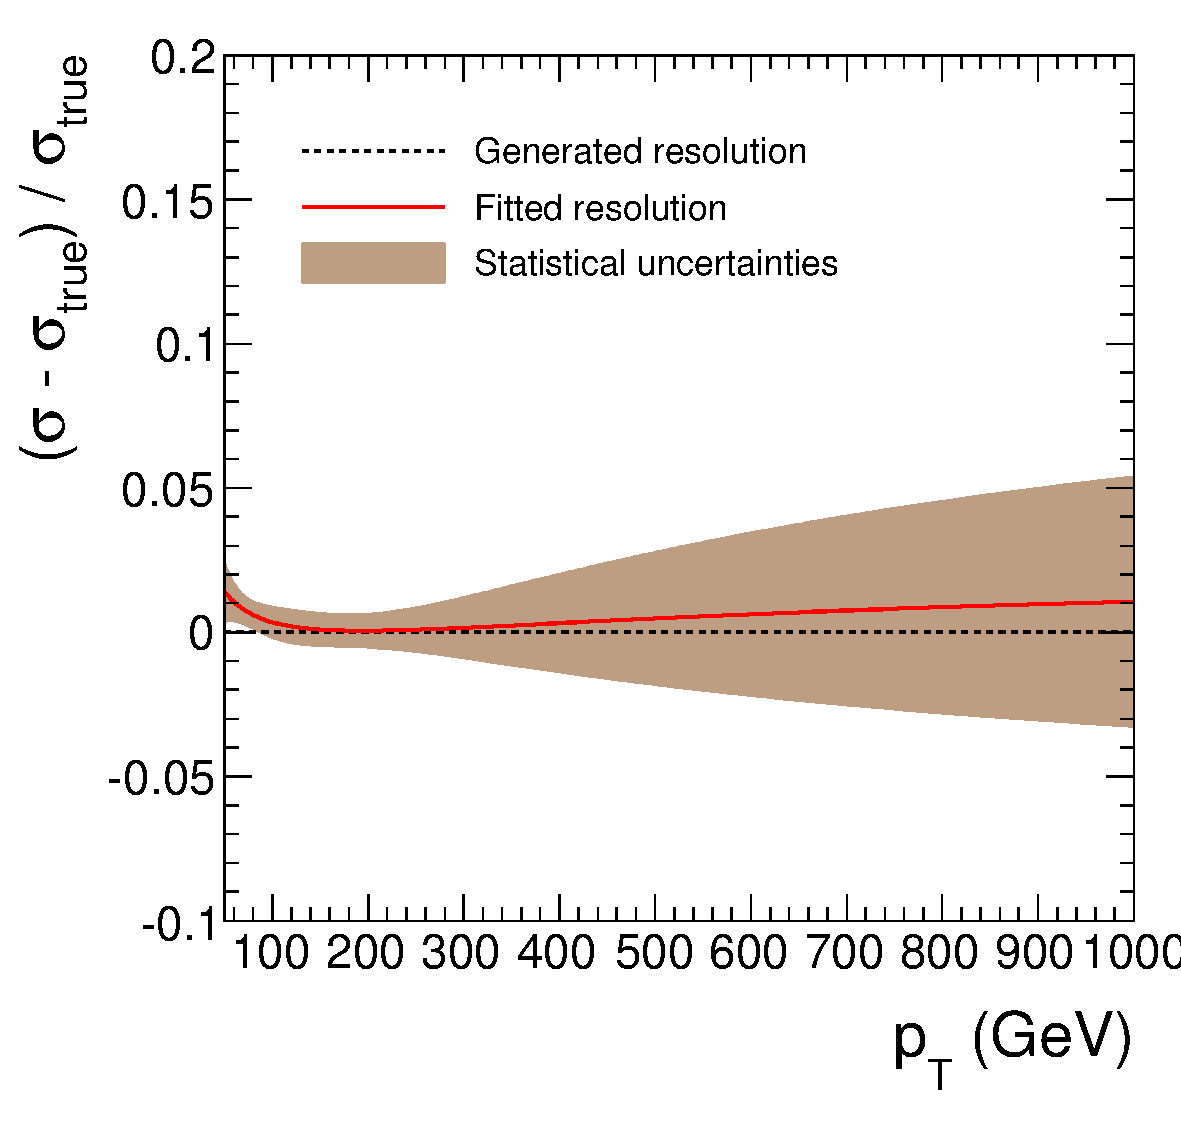
\includegraphics[width=0.45\textwidth]{figures/resFit_ToyMC_PtGenCuts_SigmaRelDifference} \\
  \end{tabular}
  \caption{(\textit{Left}) Relative Gaussian resolution $\sigma(\pt)/\pt$ evaluated with the fitted
    parameter values (solid line) in comparison to the true resolution
    (dashed line) and (\textit{right}) the relative difference
    $\sigma_{\text{fit}} / \sigma_{\text{true}}$.
    The shaded areas represent the propagated statistical
    uncertainty on the fitted parameter values, taking into account the
    parameter correlations.}
  \label{fig:ResFit:App:ToyMC:PtGenCuts:FittedSigma}
\end{figure}

The Gaussian resolution $\sigma(\pt)/\pt$ evaluated with the fitted
parameter values is shown in Fig.~\ref{fig:ResFit:App:ToyMC:PtGenCuts:FittedSigma}
in comparison to the true width at generation.
There is good agreement between the fitted and the true resolution.
The uncertainties are about $1\%$ at low \pt rising to
about $3\%$ at $\pt \approx 600\gev$ where there is sufficient statistics in
the generated sample (comp. Fig~\ref{fig:ResFit:App:ToyMC:Sample:Spectrum}).
For larger \pt the uncertainties rise up to $4.5\%$.

An example of the resulting response distribution in comparison to the true
distribution is shown in Fig.~\ref{fig:ResFit:App:ToyMC:PtGenCuts:Response} for
two different \pttrue bins.


\subsection{Measurement of the resolution with a data driven event
  selection}\label{sec:ResFit:App:ToyMC:PtCaloCuts}

The modification of the maximum likelihood method for a data driven
event selection discussed in Section~\ref{sec:ResFit:Method:Biases} is
tested using the Toy Monte Carlo simulation.
Events are selected by requiring the measured \pt of the
first\footnote{This is that one jet of the two leading jets the
  selection requirement is placed on, i.e. not necessarily the leading
  jet (comp. Section~\ref{sec:ResFit:Method:Biases}).} jet to
meet \mbox{$\ptmin = 80 < \pti{1} < \ptmax = 800\gev$} (comp. Fig.~\ref{fig:ResFit:App:ToyMC:PtCuts:Spectrum}).

\begin{figure}[ht]
  \centering
  \begin{tabular}{cc}
    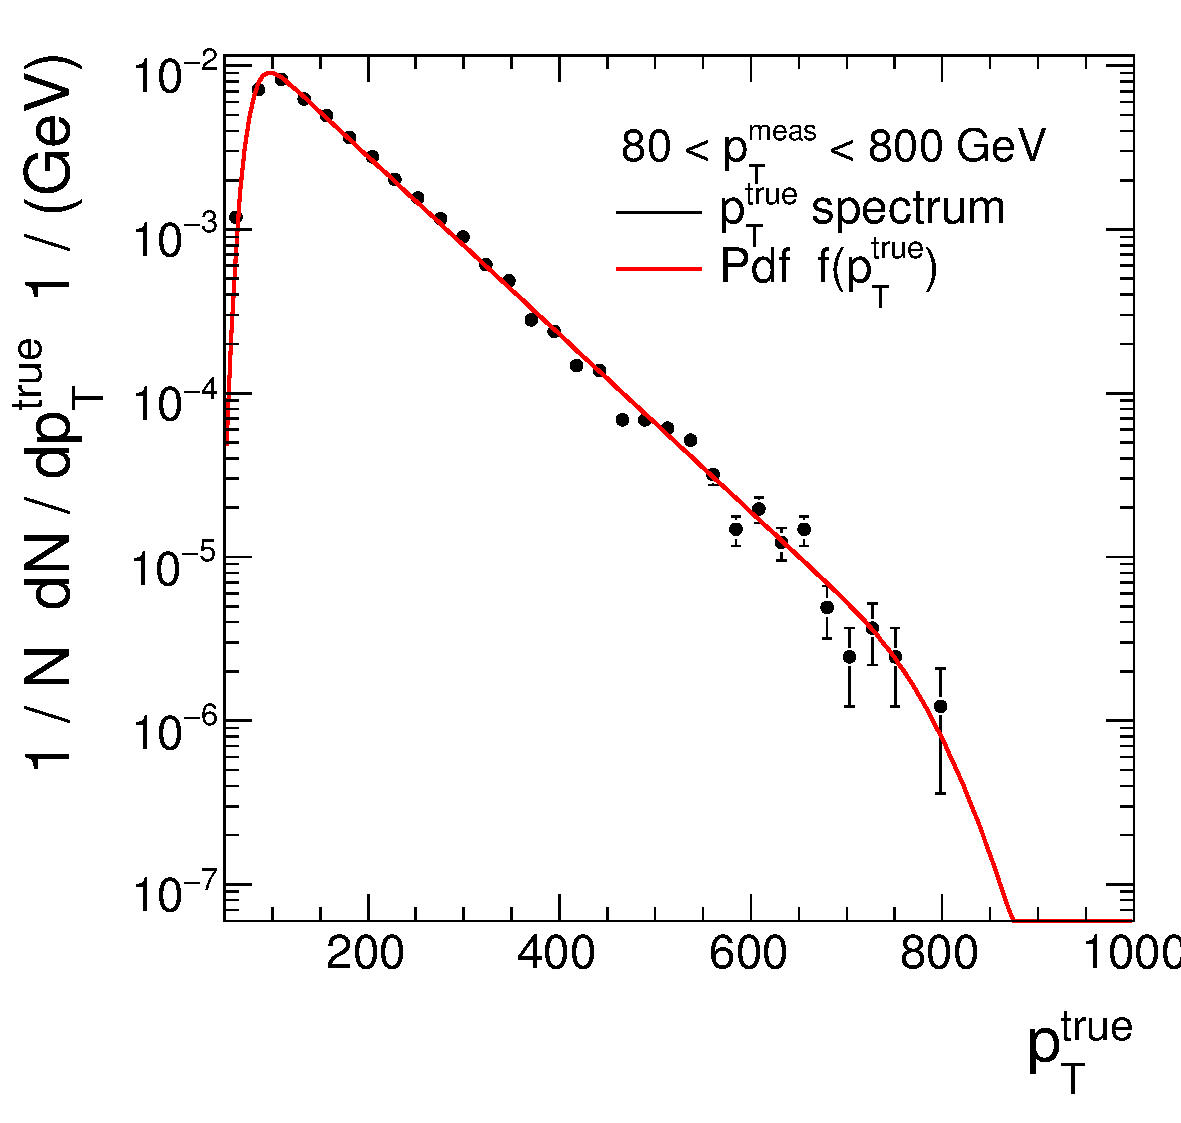
\includegraphics[width=0.45\textwidth]{figures/resFit_ToyMC_PtCuts_SpectrumLog} &
    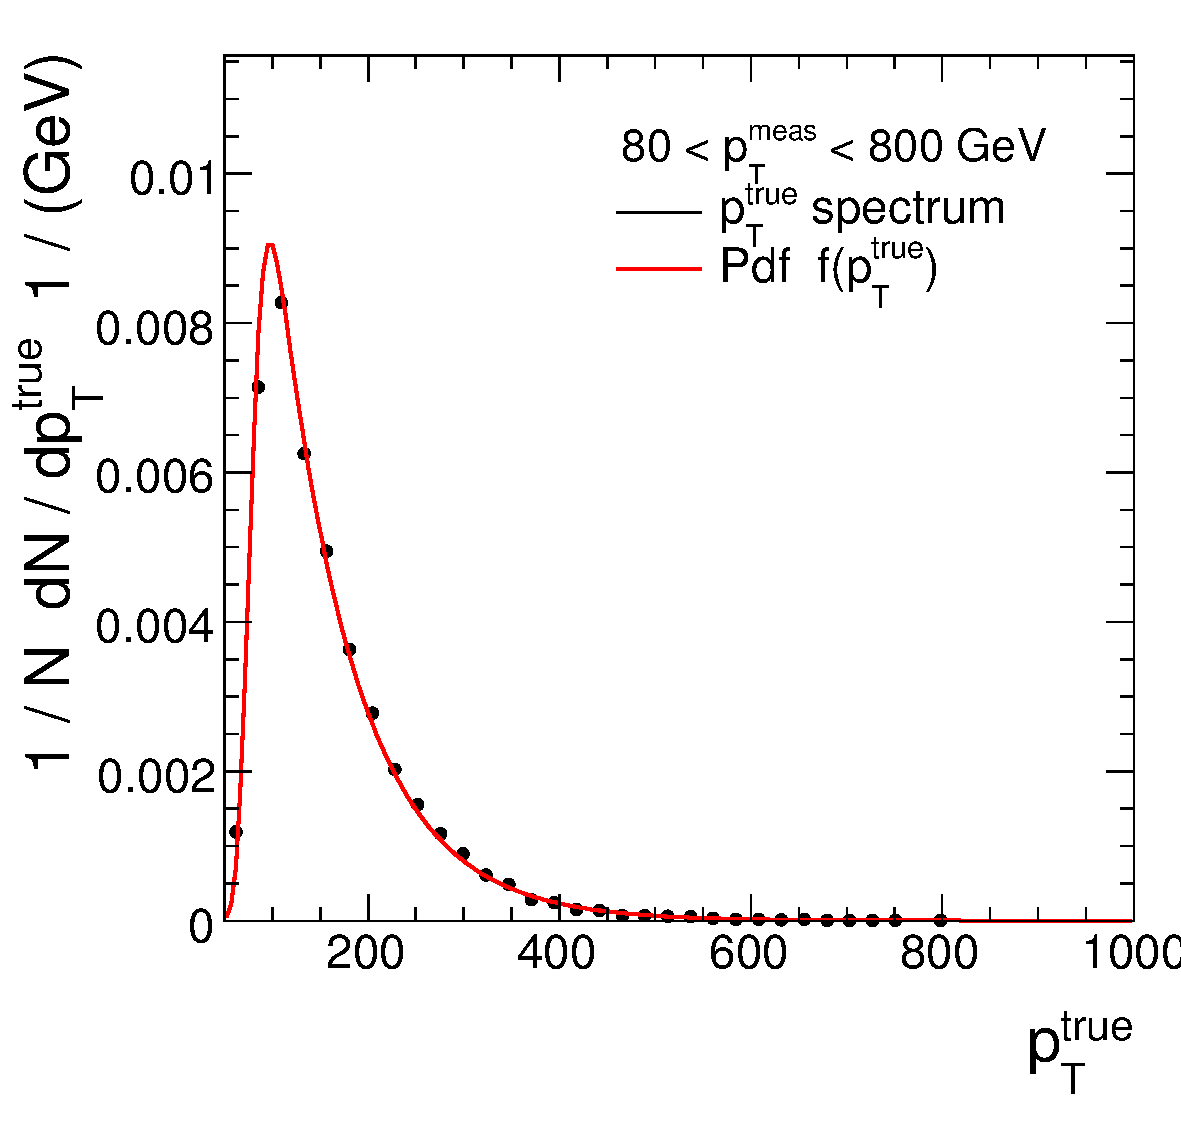
\includegraphics[width=0.45\textwidth]{figures/resFit_ToyMC_PtCuts_SpectrumLinear} \\
  \end{tabular}
  \caption{Demonstration of the migration effects caused by a data
    driven event selection.
    Shown is the \pttrue spectrum (circular markers) after
    requiring \mbox{$80 < \pt < 800\gev$}, in linear scale
    (\textit{left}) and logarithmic scale scale (\textit{right}).
    The spectrum is well described by the modified pdf
    $\tilde{f}(\pttrue)$.
    (Compare the underlying spectrum Fig.~\ref{fig:ResFit:App:ToyMC:Sample:Spectrum}.)
  }
  \label{fig:ResFit:App:ToyMC:PtCuts:Spectrum}
\end{figure}


\begin{figure}[ht]
  \centering
  \begin{tabular}{cc}
    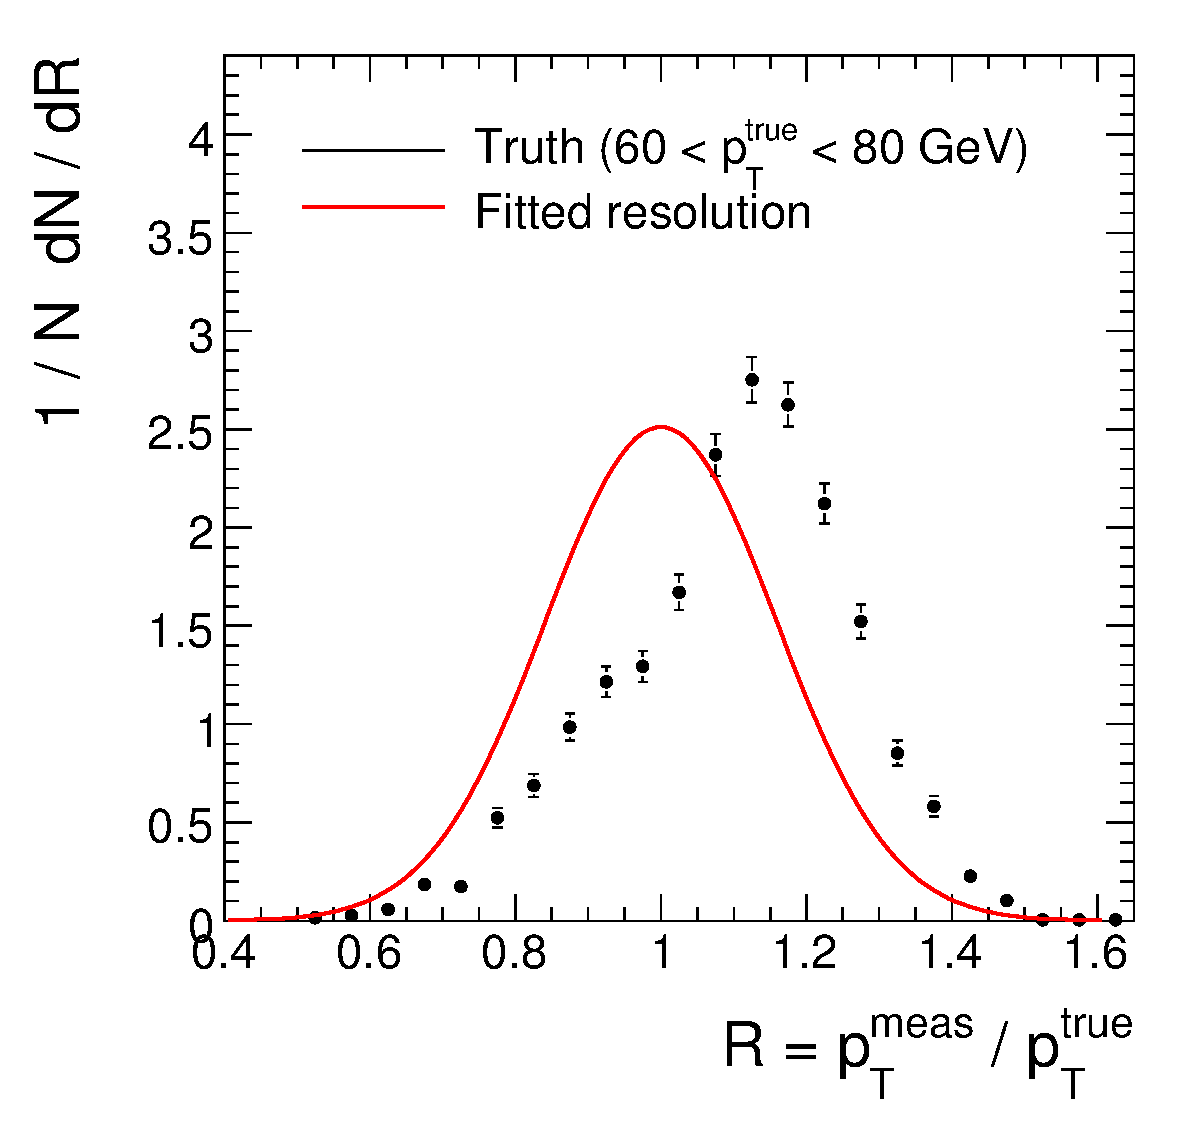
\includegraphics[width=0.45\textwidth]{figures/resFit_ToyMC_PtCuts_ResolutionBin1} &
    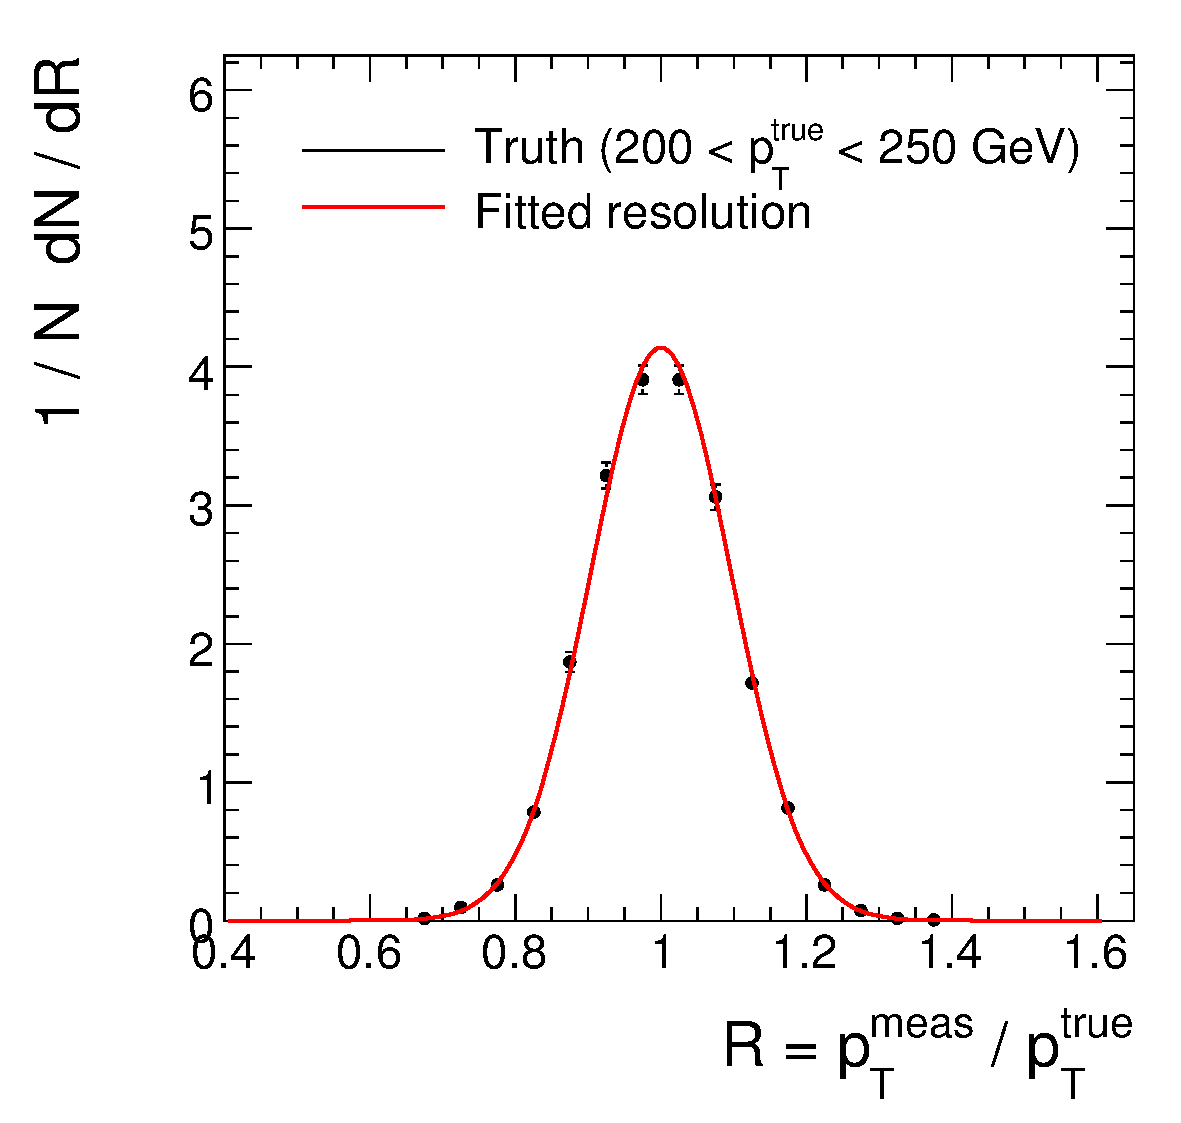
\includegraphics[width=0.45\textwidth]{figures/resFit_ToyMC_PtCuts_ResolutionBin7} \\
  \end{tabular}
  \caption{Generated Gaussian response \mbox{$\pt / \pttrue$}
    (circular markers) and the fitted
    response (solid line) in two different \pttrue bins after
    requiring \mbox{$80 < \pt < 800\gev$}.
    Note the migration effects (\textit{left}): the narrow peak at the
    right side is populated by the first jets in each event, i.e. that have been cut on, and hence these are jets fluctuating upwards into the \pt bin.
    The wider peak centred around 1 is populated by the unconstrained
    second jet.
    (There is more upward than downward fluctuation due to the falling
    \pttrue spectrum.)
  }
  \label{fig:ResFit:App:ToyMC:PtCuts:Response}
\end{figure}

\begin{figure}[ht]
  \centering
  \begin{tabular}{cc}
    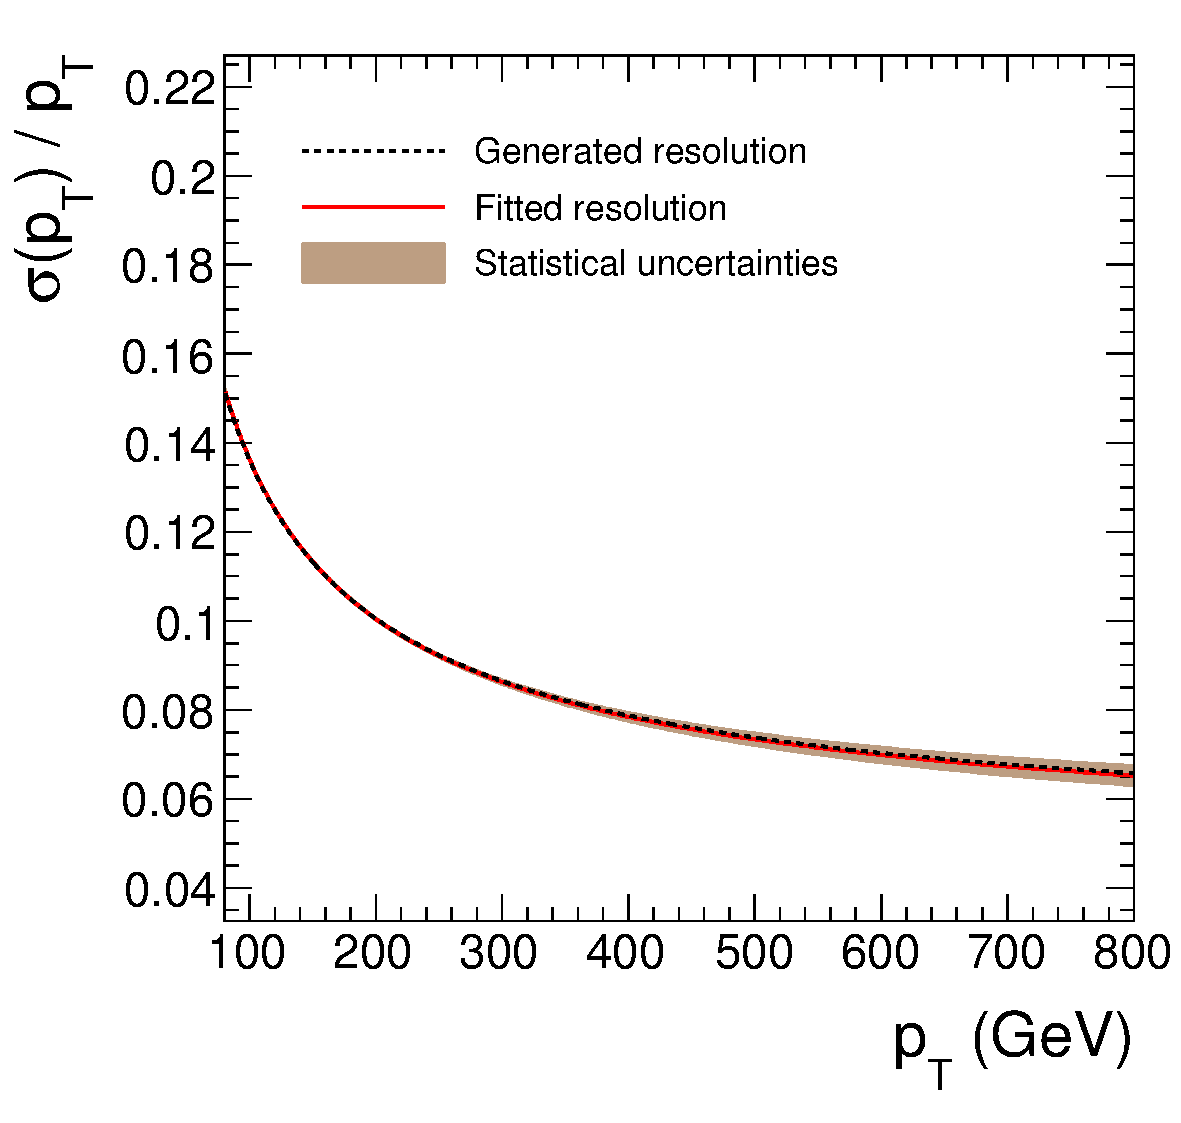
\includegraphics[width=0.45\textwidth]{figures/resFit_ToyMC_PtCuts_Sigma} &
    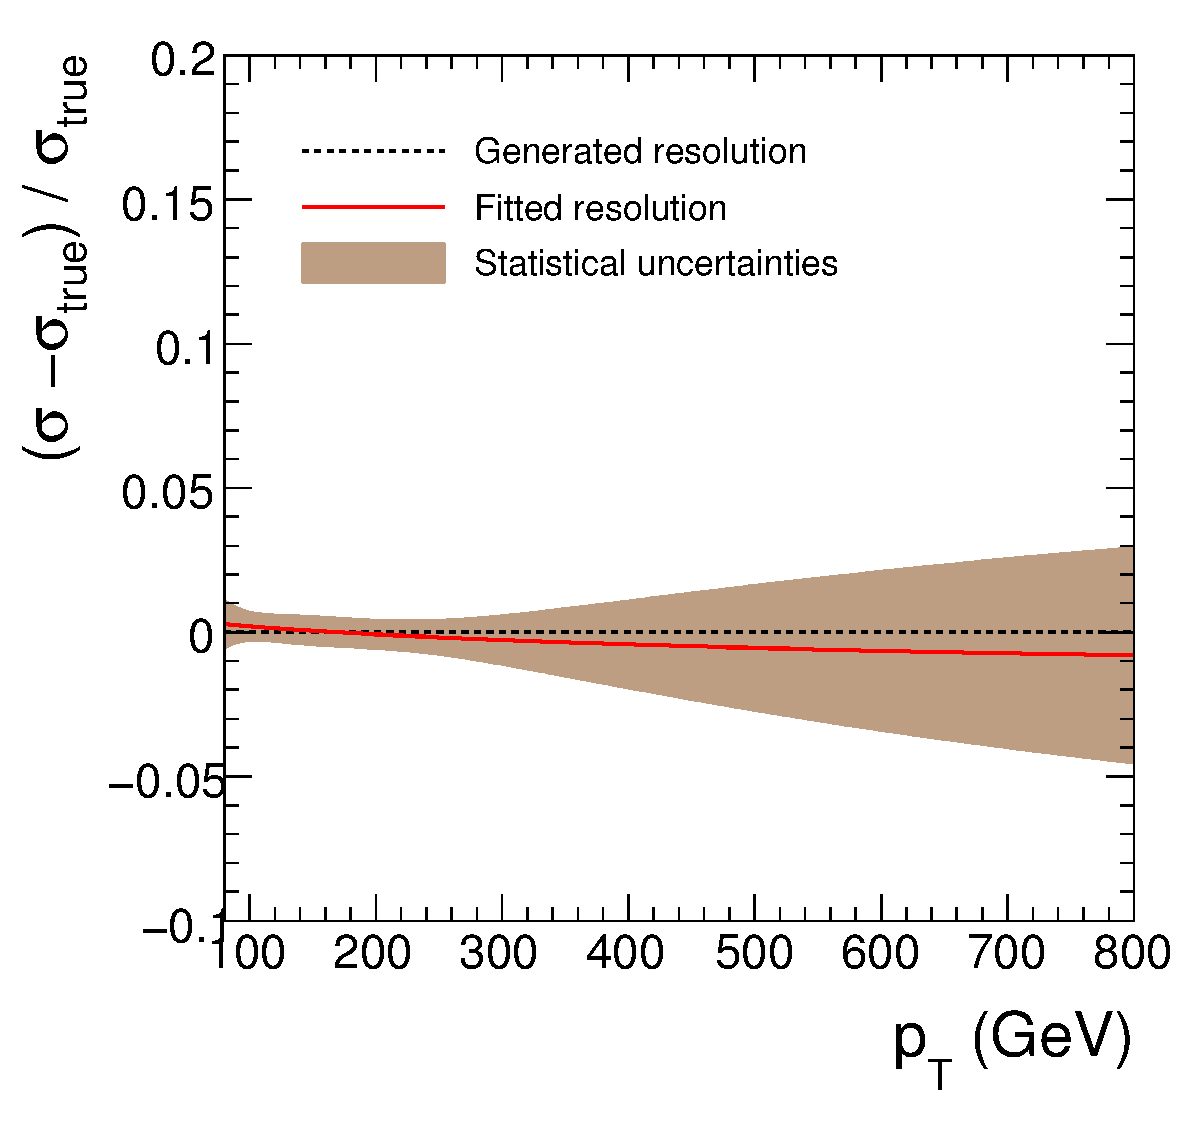
\includegraphics[width=0.45\textwidth]{figures/resFit_ToyMC_PtCuts_SigmaRelDifference} \\
  \end{tabular}
  \caption{(\textit{Left}) Relative Gaussian resolution $\sigma(\pt)/\pt$ evaluated with the fitted
    parameter values (solid line) in comparison to the true resolution
    (dashed line) and (\textit{right}) the relative difference
    $\sigma_{\text{fit}} / \sigma_{\text{true}}$.
    The shaded areas represent the propagated statistical
    uncertainty on the fitted parameter values, taking into account the
    parameter correlations.
    The fit has been performed with dijet events selected by requiring \mbox{$80 < \pt < 800\gev$}.}
  \label{fig:ResFit:App:ToyMC:PtCuts:FittedSigma}
\end{figure}


\begin{table}[ht]
  \caption{Parameter values of the Gaussian jet \pt resolution
    $\sigma$.
    Listed are the true values used for the generation and
    the fitted values.
    The uncertainties assigned to the fitted values
    are the statistical uncertainties from the fit.
    The fit has been performed with dijet events selected by requiring
    \mbox{$80 < \pt < 800\gev$}.}
  \centering
  \begin{tabular}[ht]{lccc}
    \toprule
    $b_{i}$ & $0$ & $1$ & $2$ \\
    \midrule
    True value & $4$           & $1.2$                   & $0.05$ \\
    Fit result   & $4 \pm 1$ & $1.20 \pm 0.07$ & $0.049 \pm 0.005$ \\
    \bottomrule
   \end{tabular}
 \label{tab:ResFit:ToyMC:PtCuts:FitResult}
\end{table}


The fitted parameter values $\mathbf{\xi}$ of the Gaussian resolution $\sigma$ are listed in Tab.~\ref{tab:ResFit:ToyMC:PtCuts:FitResult}.
They agree with the true values within the statistical uncertainties.
As expected, they feature the same correlation pattern as in the
fitted parameters in Section~\ref{sec:ResFit:App:ToyMC:PtGenCuts}.

The relative Gaussian resolution $\sigma(\pt)/\pt$ evaluated with the fitted parameter values is shown in Fig.~\ref{sec:ResFit:App:ToyMC:PtGenCuts} in comparison to the true resolution at generation.
There is good agreement within the statistical uncertainties.
As before, the uncertainties are about $1\%$ at low \pt rising to about $3\%$ at $\pt \approx 600\gev$ and up to $4.5\%$ at very large \pt.
An example of the resulting response distributions is shown in
Fig.~\ref{fig:ResFit:App:ToyMC:PtCuts:Response} for two \pttrue bins.

From the results presented in this section, it is concluded that the
maximum likelihood method is suited to measure the jet \pt resolution
of dijets that are perfectly balanced in \pttrue.

\section{Fit results for all \pt and $\eta$ bins}\label{sec:ResFit:App:AllResults}
\subsection{Gaussian response function}\label{sec:ResFit:App:AllResults:Gauss}

% ----- Gauss Eta0 Spectra -----
\begin{figure}[ht]
  \centering
  \begin{tabular}{ccc}
    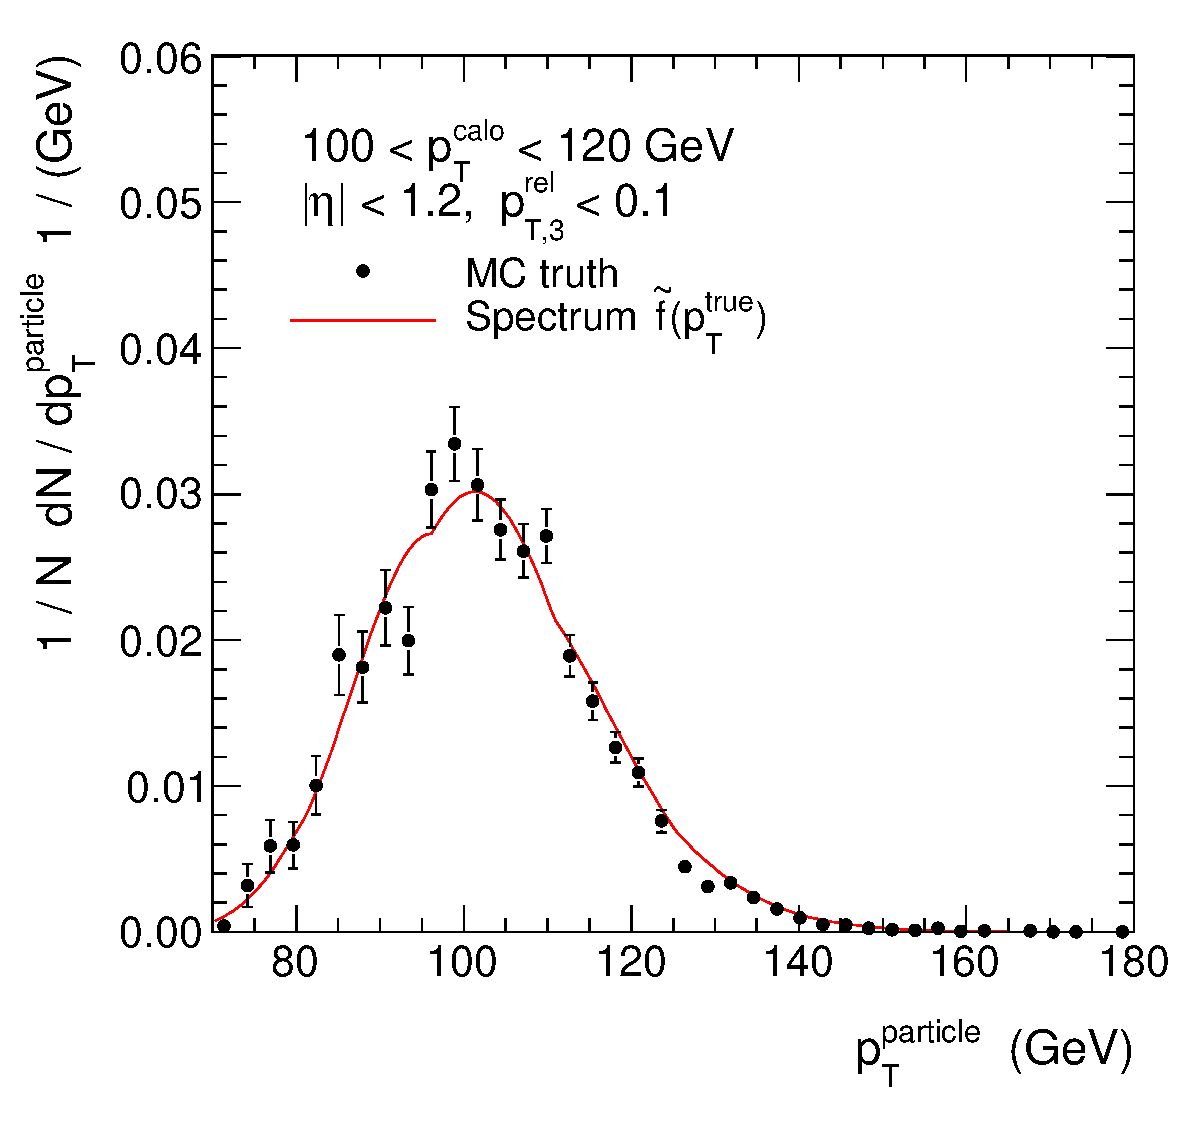
\includegraphics[width=0.3\textwidth]{figures/ResFit_Spring10QCDFlat_Gauss_Eta0_Spectrum_PtBin1} &
    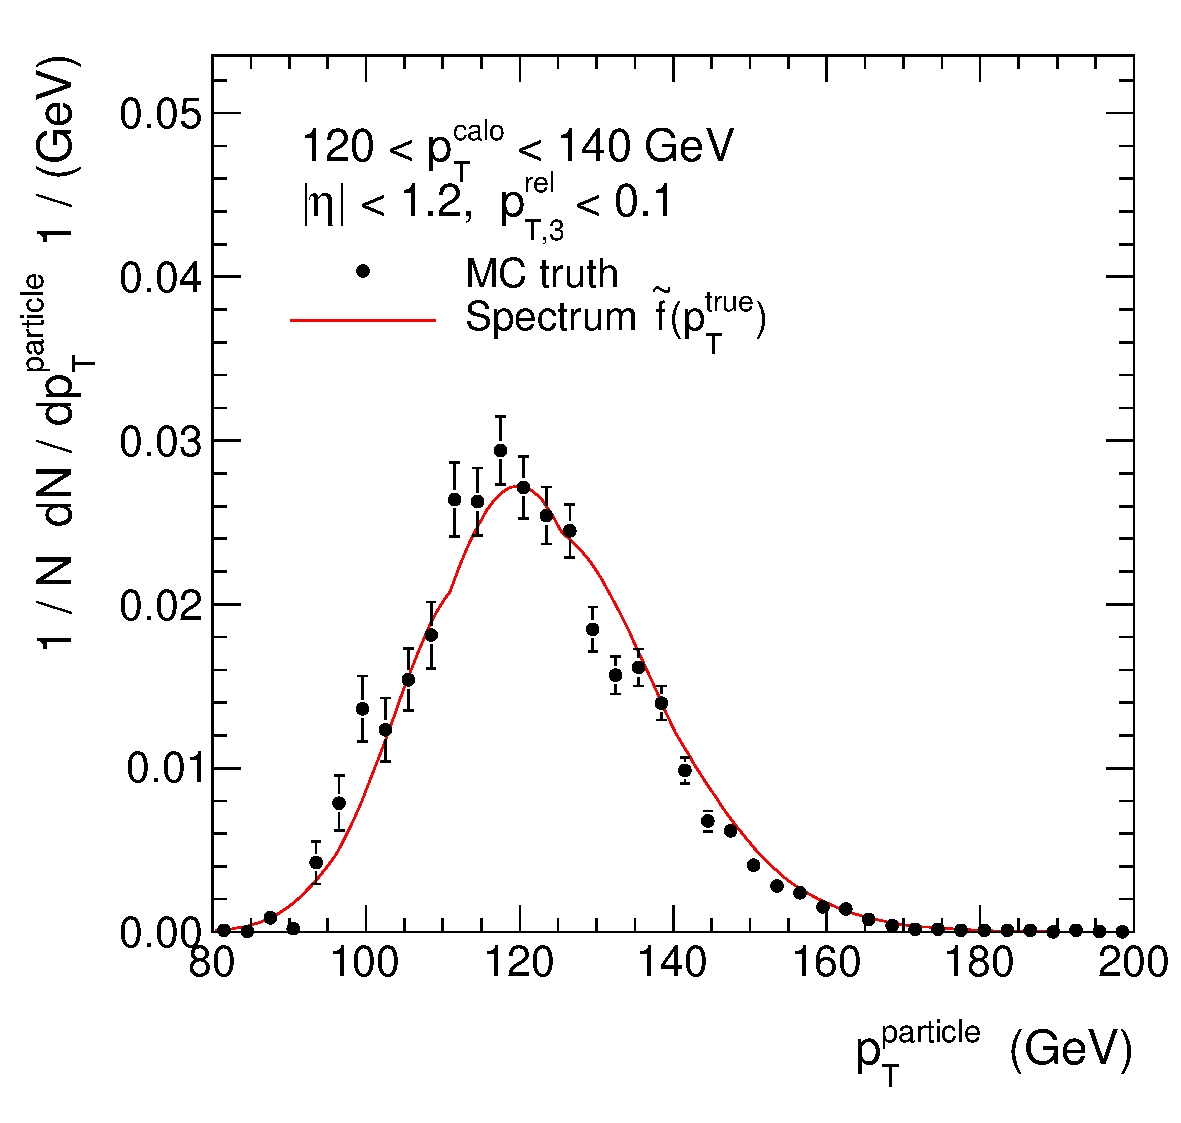
\includegraphics[width=0.3\textwidth]{figures/ResFit_Spring10QCDFlat_Gauss_Eta0_Spectrum_PtBin2} &
    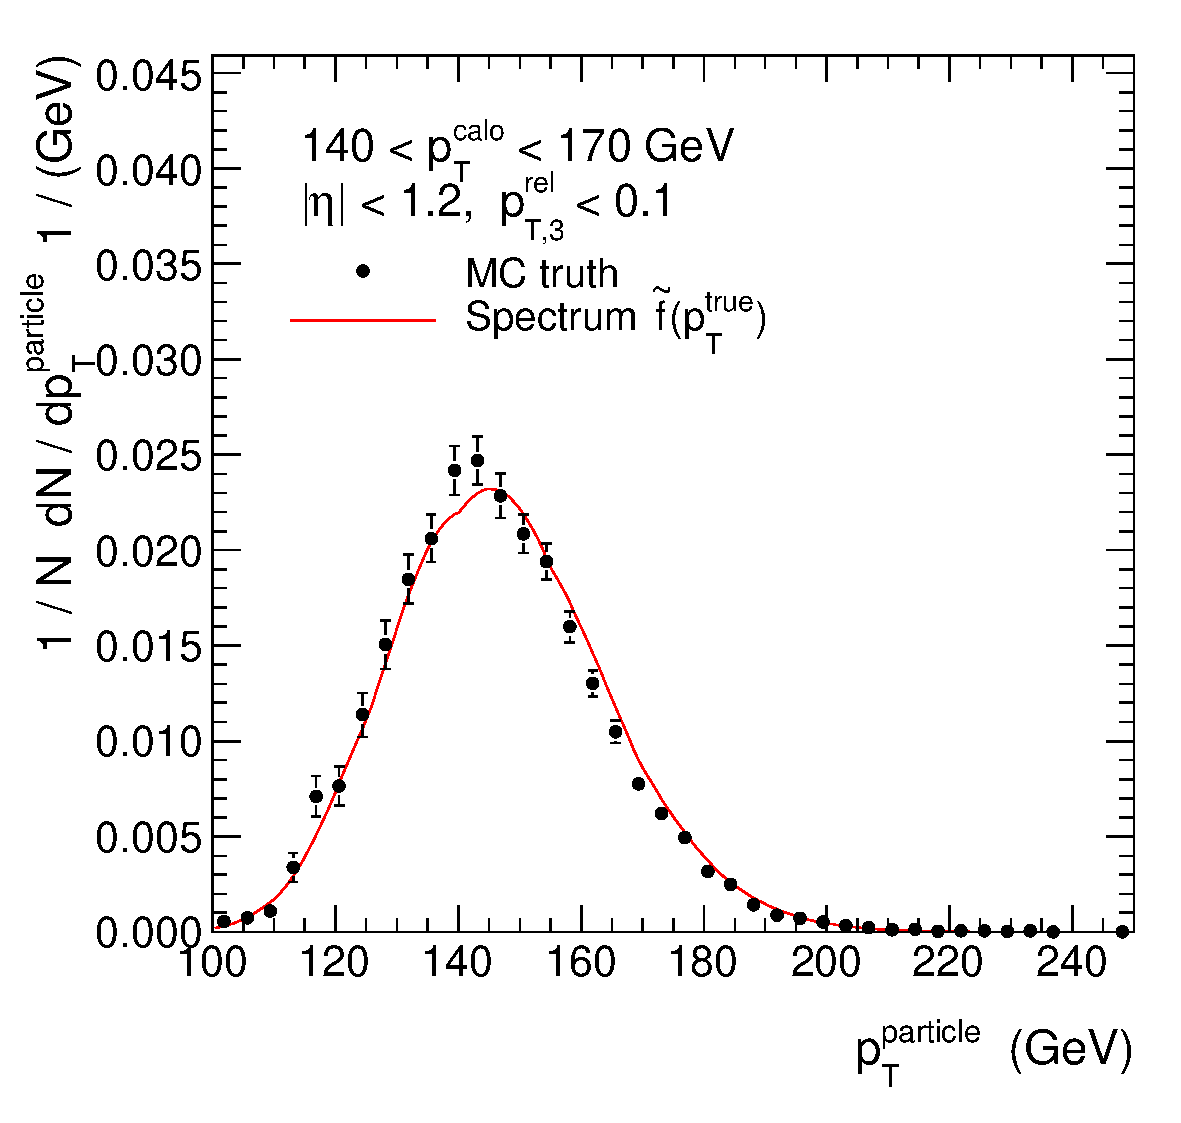
\includegraphics[width=0.3\textwidth]{figures/ResFit_Spring10QCDFlat_Gauss_Eta0_Spectrum_PtBin3} \\

    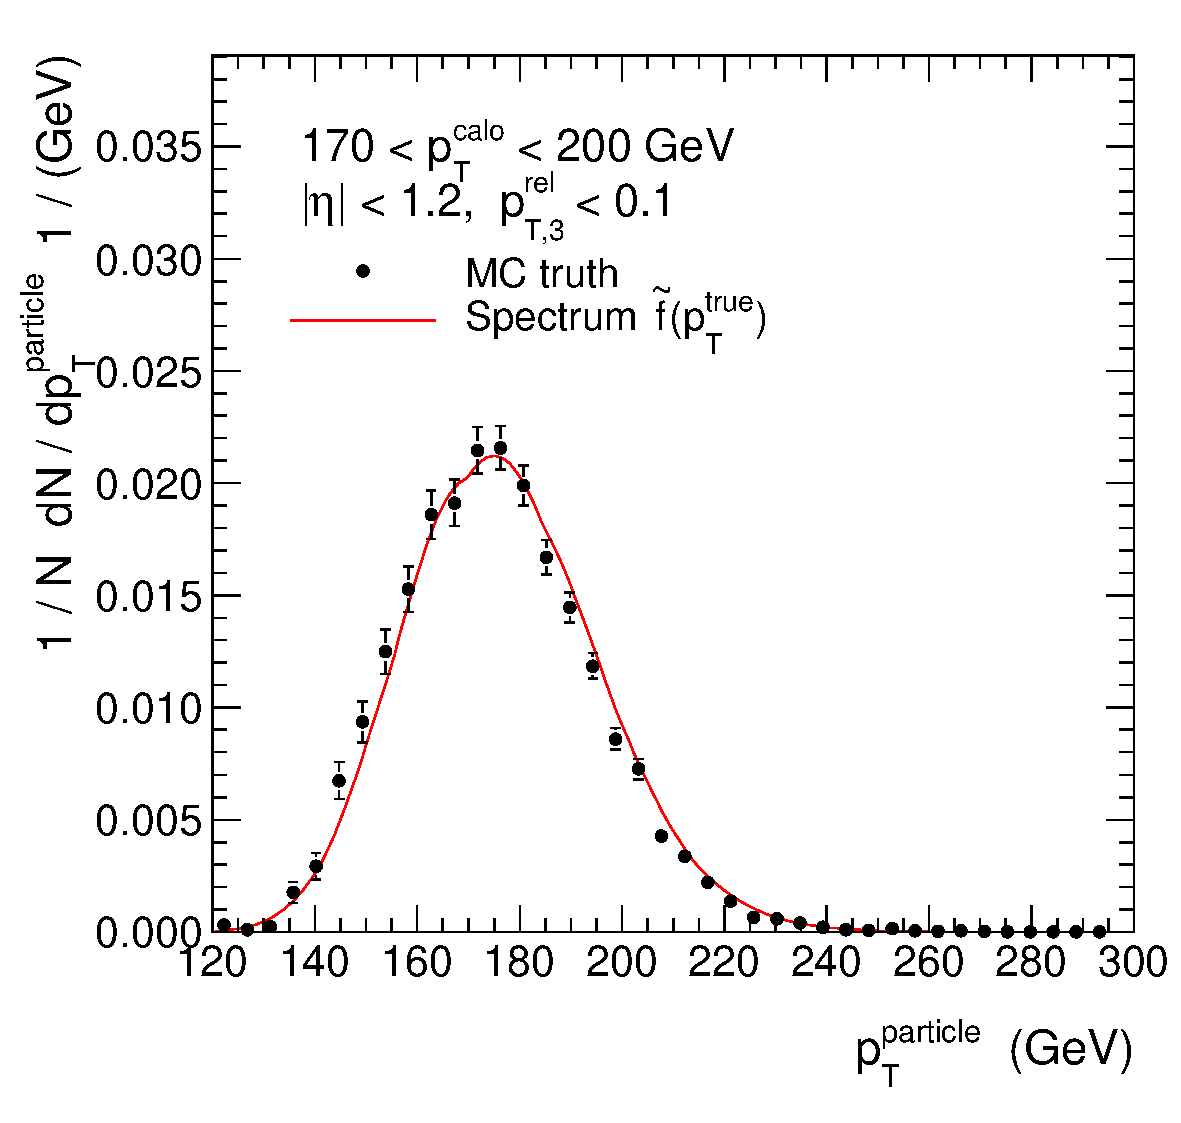
\includegraphics[width=0.3\textwidth]{figures/ResFit_Spring10QCDFlat_Gauss_Eta0_Spectrum_PtBin4} &
    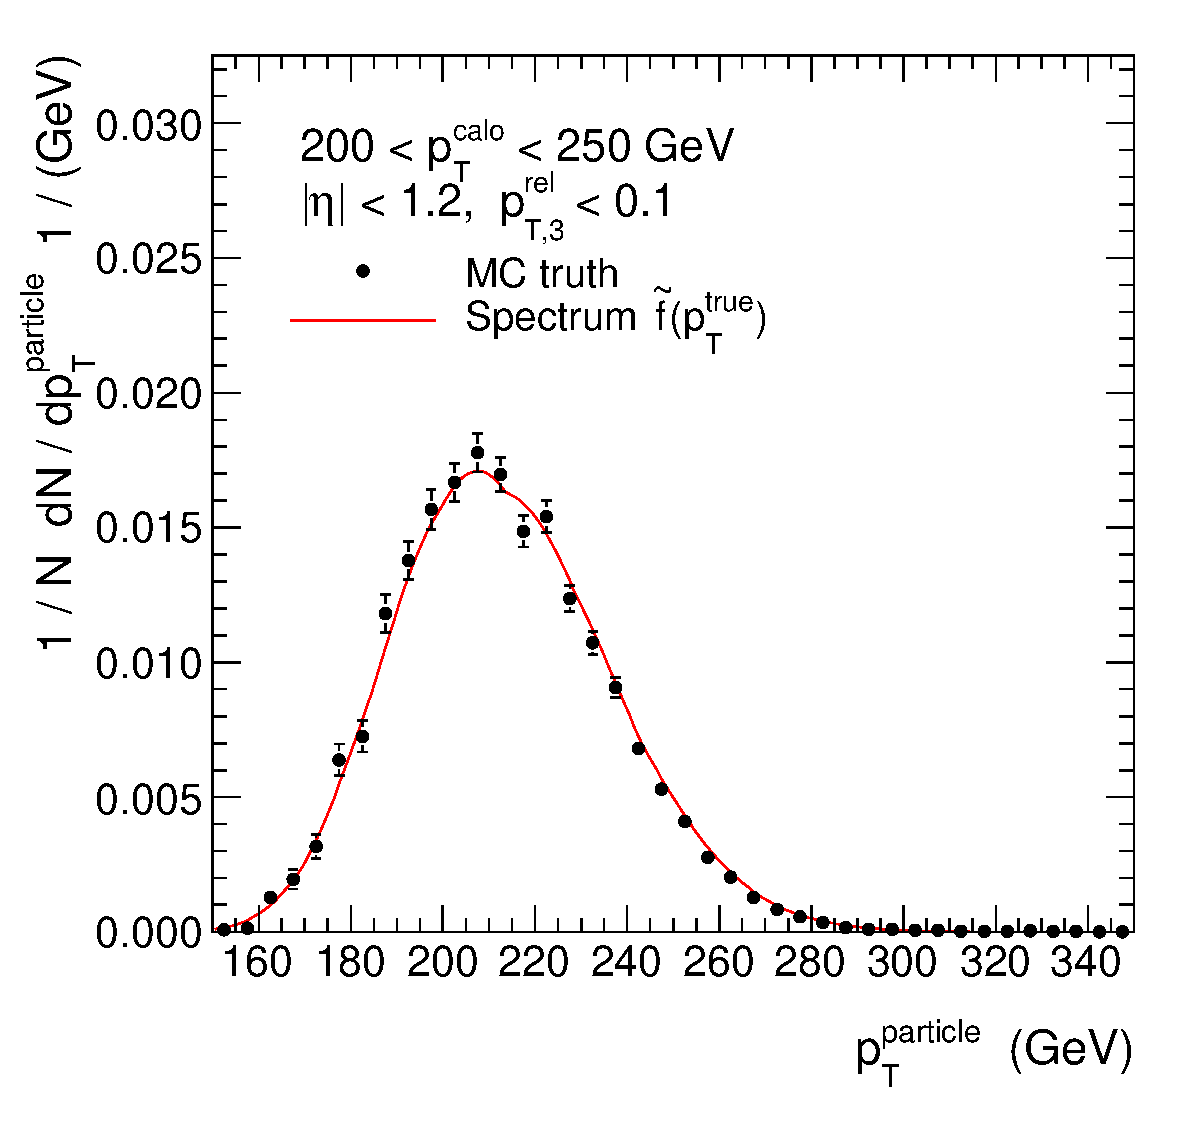
\includegraphics[width=0.3\textwidth]{figures/ResFit_Spring10QCDFlat_Gauss_Eta0_Spectrum_PtBin5} &
    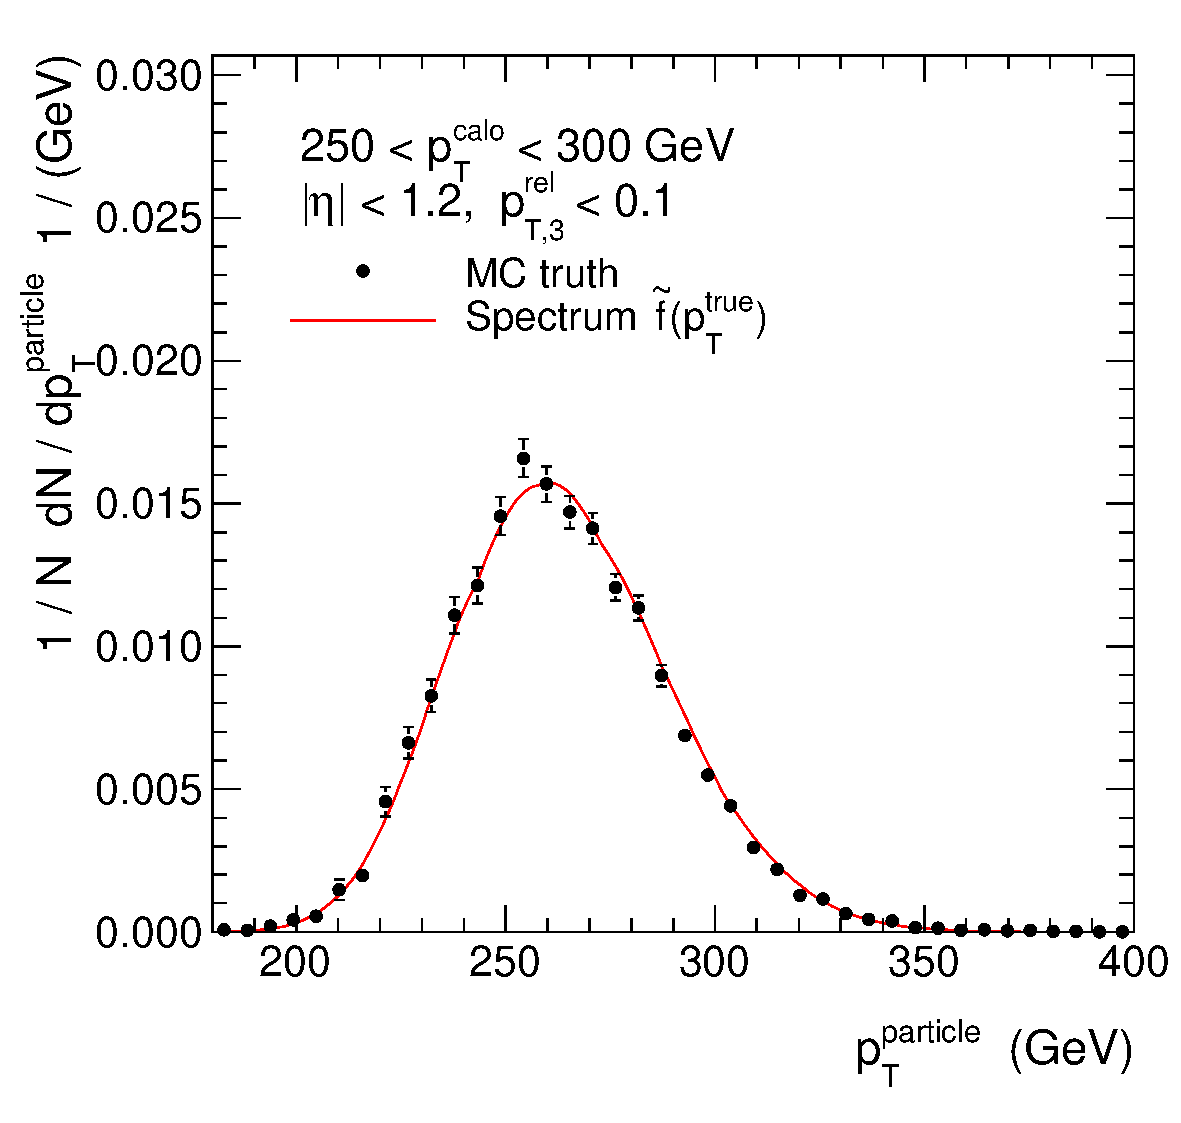
\includegraphics[width=0.3\textwidth]{figures/ResFit_Spring10QCDFlat_Gauss_Eta0_Spectrum_PtBin6} \\

    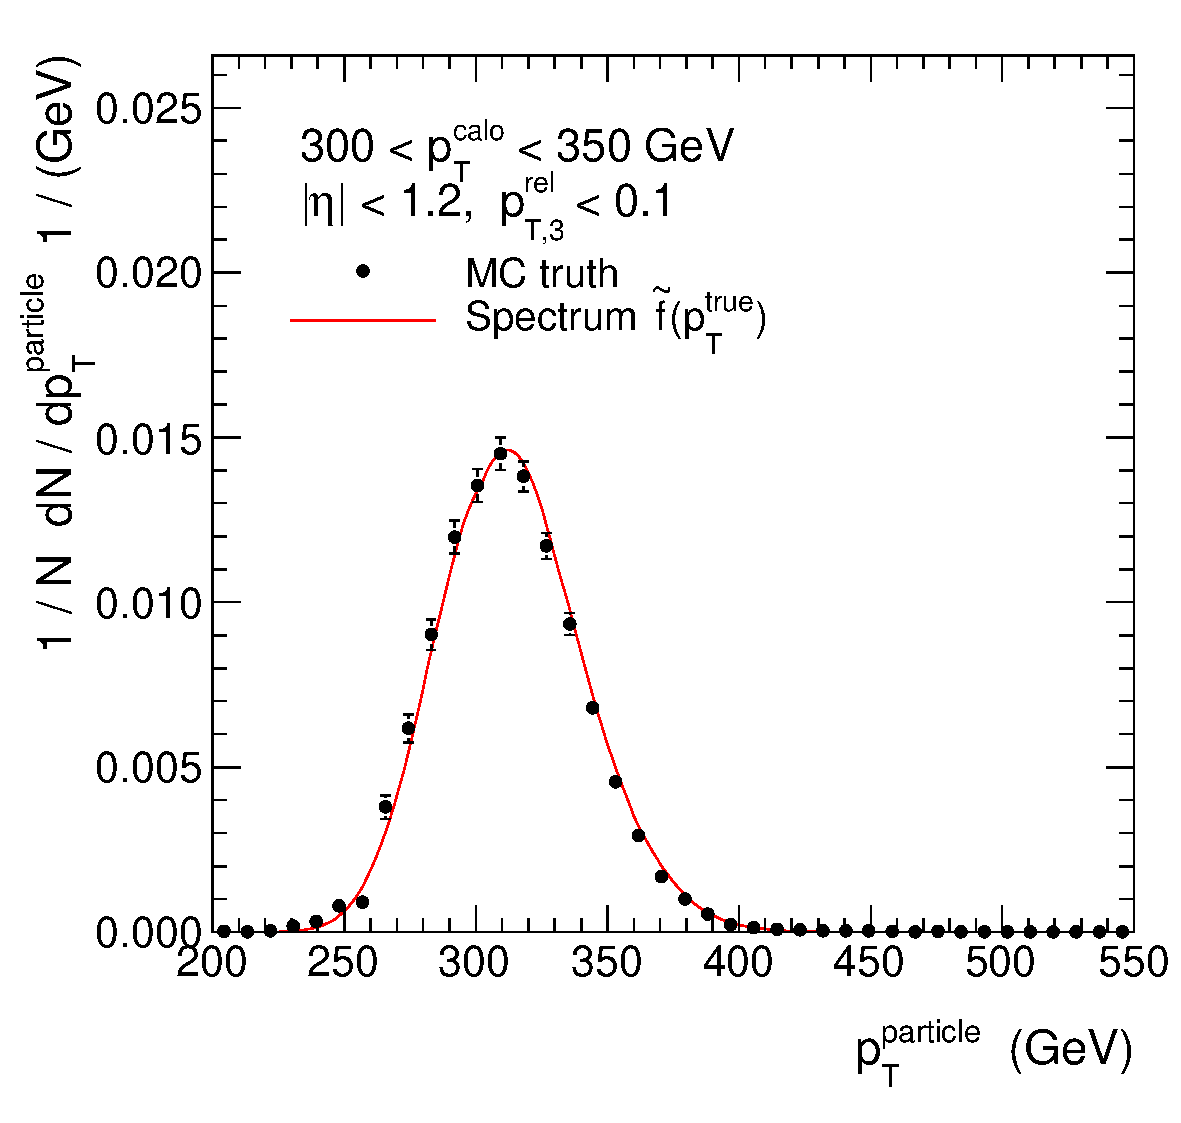
\includegraphics[width=0.3\textwidth]{figures/ResFit_Spring10QCDFlat_Gauss_Eta0_Spectrum_PtBin7} &
    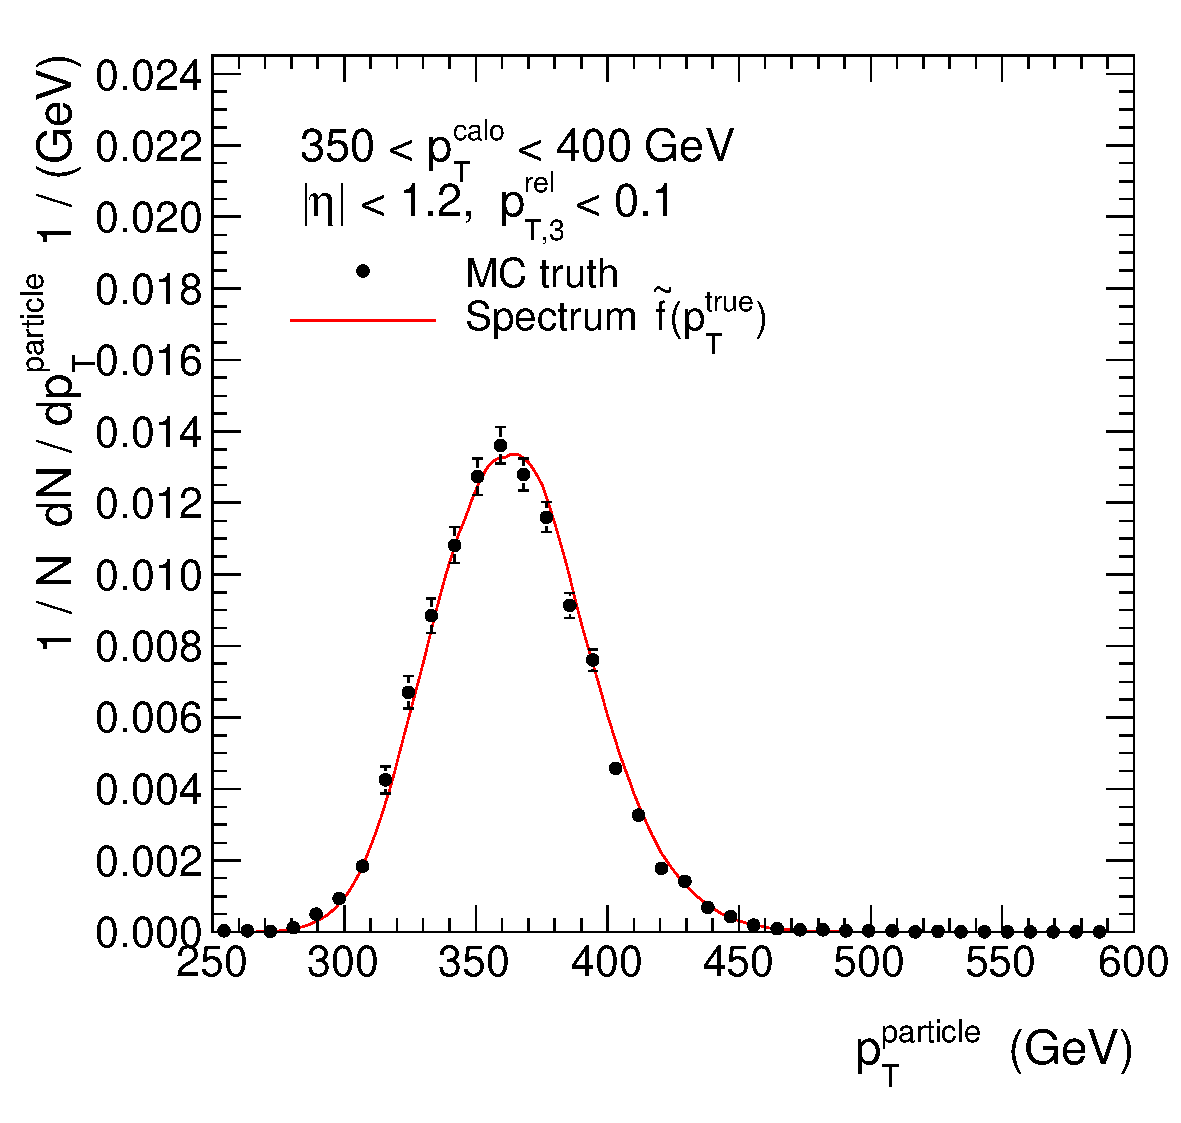
\includegraphics[width=0.3\textwidth]{figures/ResFit_Spring10QCDFlat_Gauss_Eta0_Spectrum_PtBin8} &
    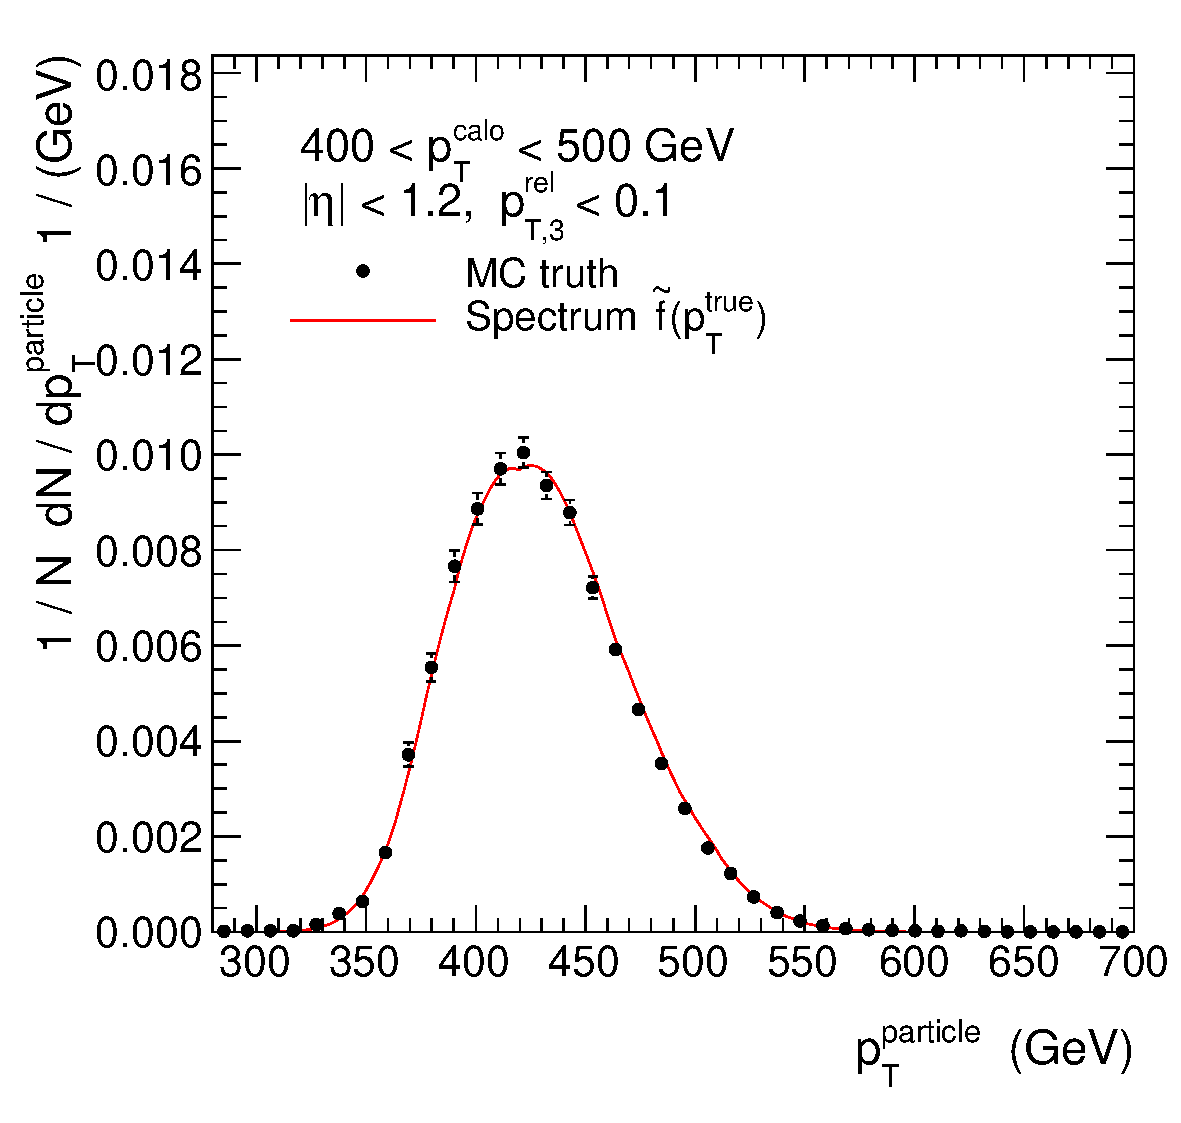
\includegraphics[width=0.3\textwidth]{figures/ResFit_Spring10QCDFlat_Gauss_Eta0_Spectrum_PtBin9} \\

    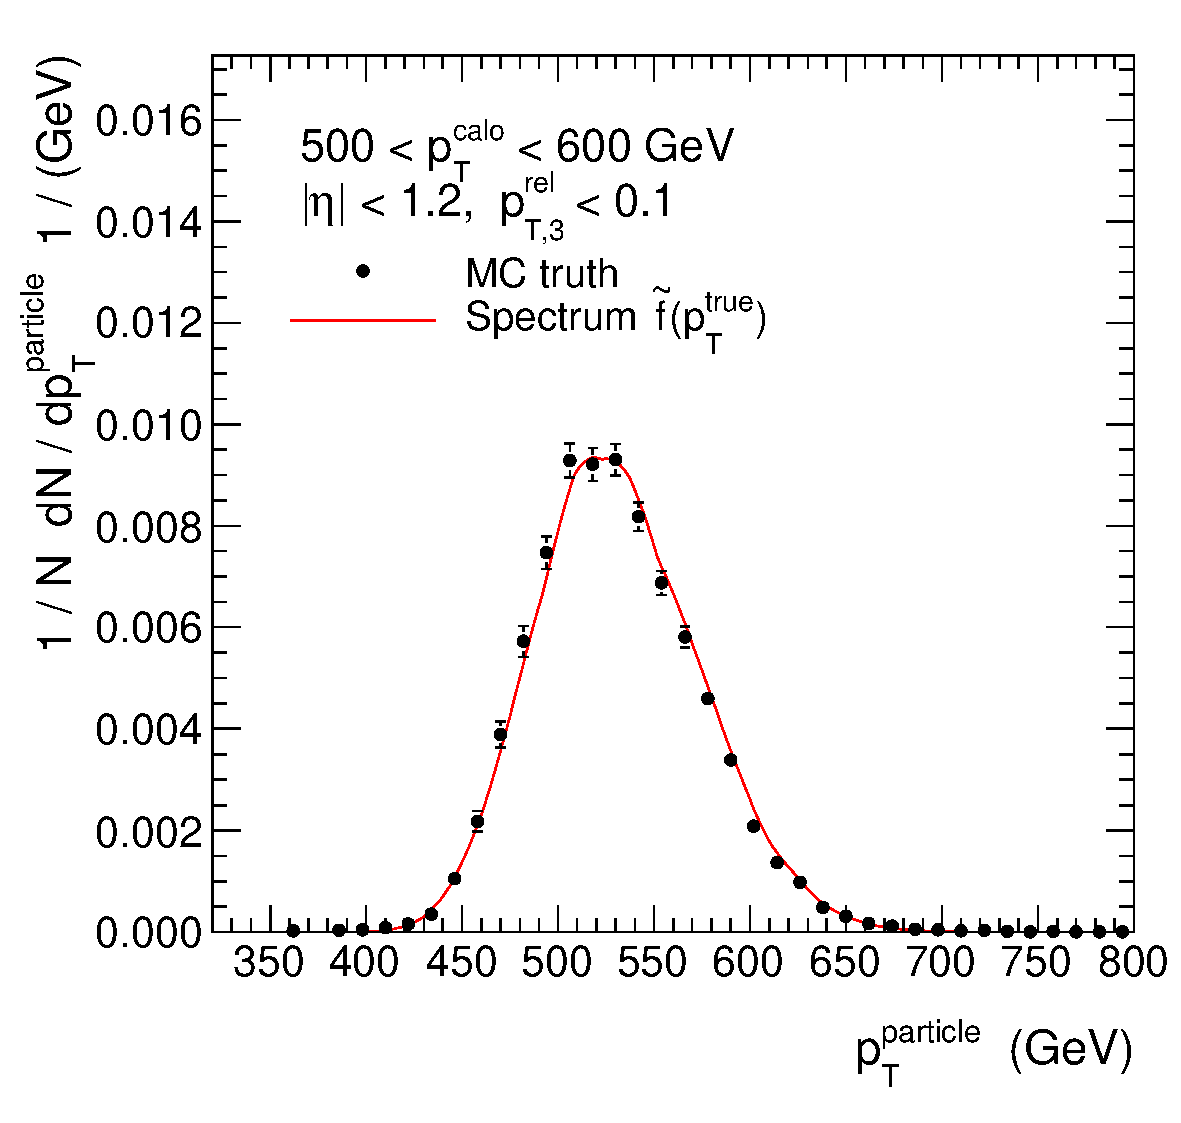
\includegraphics[width=0.3\textwidth]{figures/ResFit_Spring10QCDFlat_Gauss_Eta0_Spectrum_PtBin10} &
    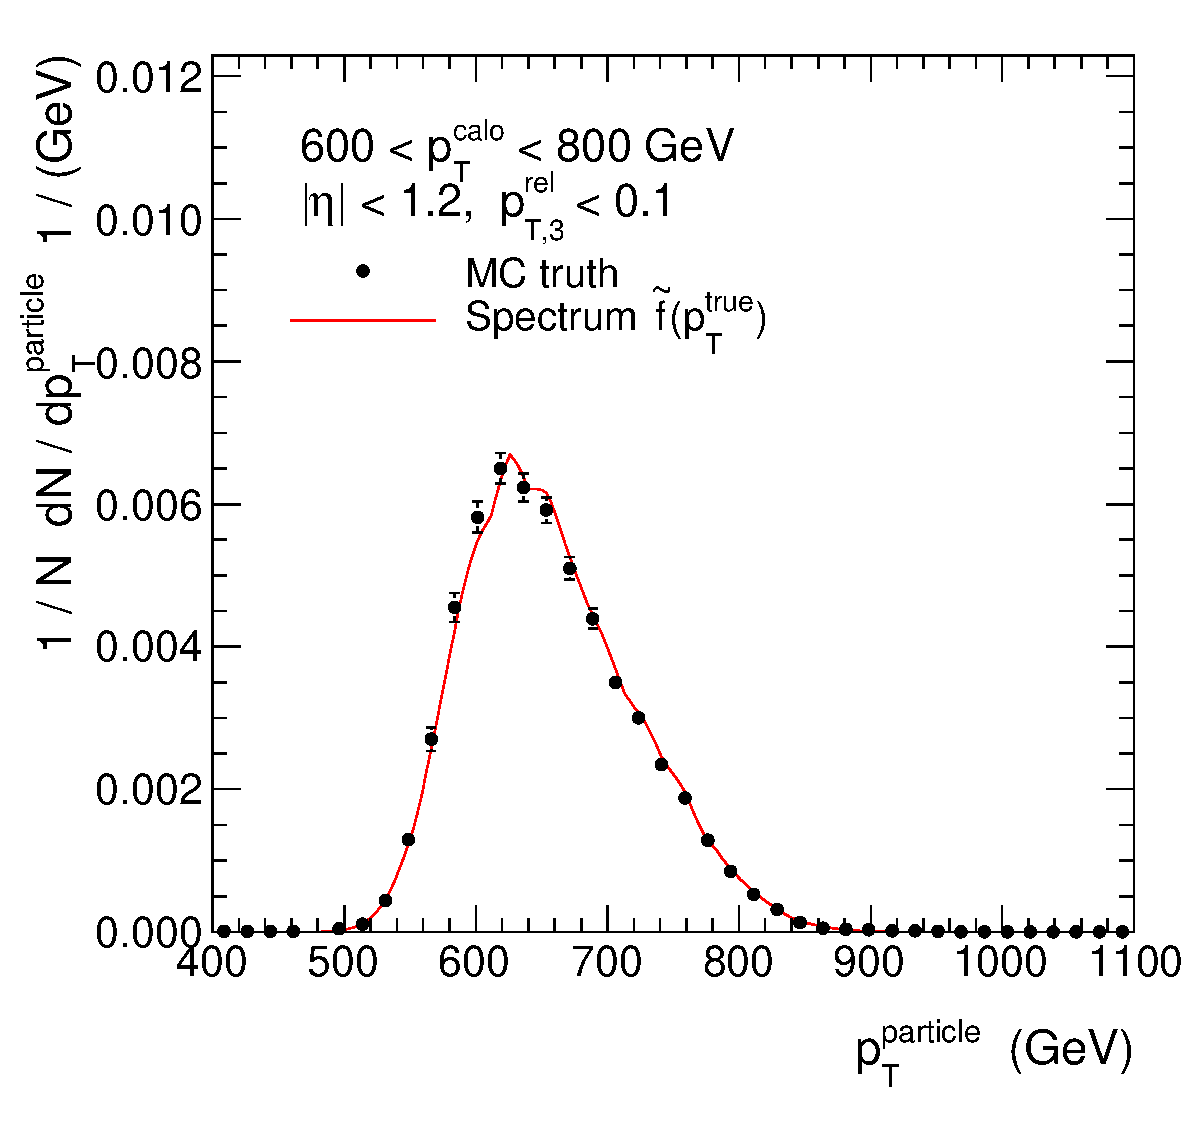
\includegraphics[width=0.3\textwidth]{figures/ResFit_Spring10QCDFlat_Gauss_Eta0_Spectrum_PtBin11} &
    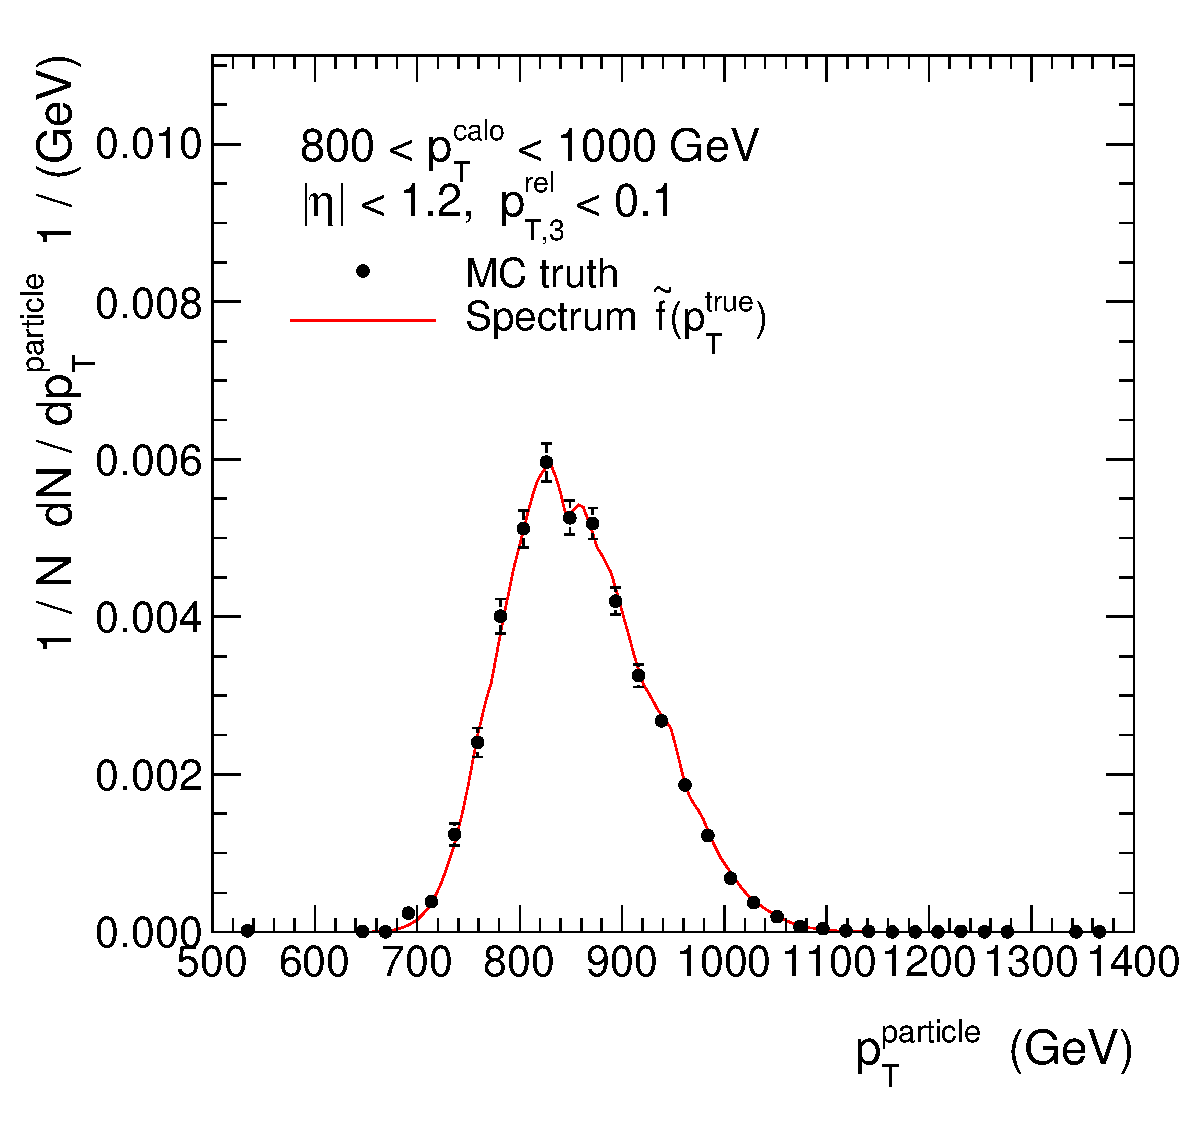
\includegraphics[width=0.3\textwidth]{figures/ResFit_Spring10QCDFlat_Gauss_Eta0_Spectrum_PtBin12} \\
  \end{tabular}
\caption{The parametrisation of the realistic particle jet \pt spectrum as used in the dijet likelihood (solid line) in comparison to the prediction from Monte Carlo truth (full circles) in different \pt bins for \mbox{$|\eta|<1.2$}. Migration effects are modelled assuming a Gaussian response function.}
\label{fig:ResFit:App:Gauss:Spectrum}
\end{figure}


% ----- Gauss Eta0 Extrapolations -----
\begin{figure}[ht]
  \centering
  \begin{tabular}{ccc}
    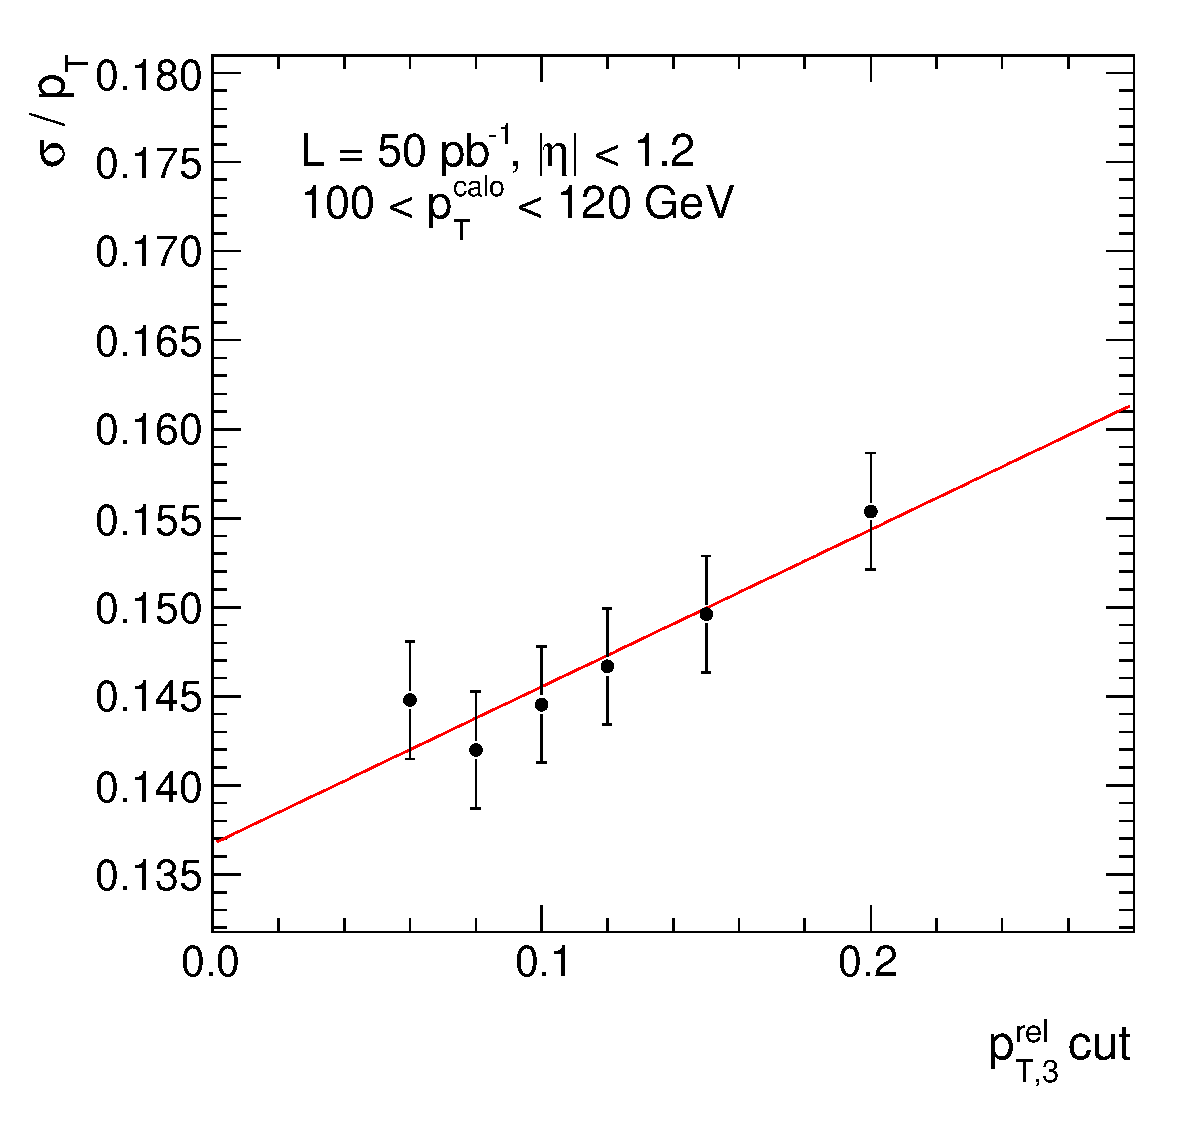
\includegraphics[width=0.3\textwidth]{figures/ResFit_Spring10QCDFlat_Gauss_Eta0_ExtrapolatedPar0_PtBin1} &
    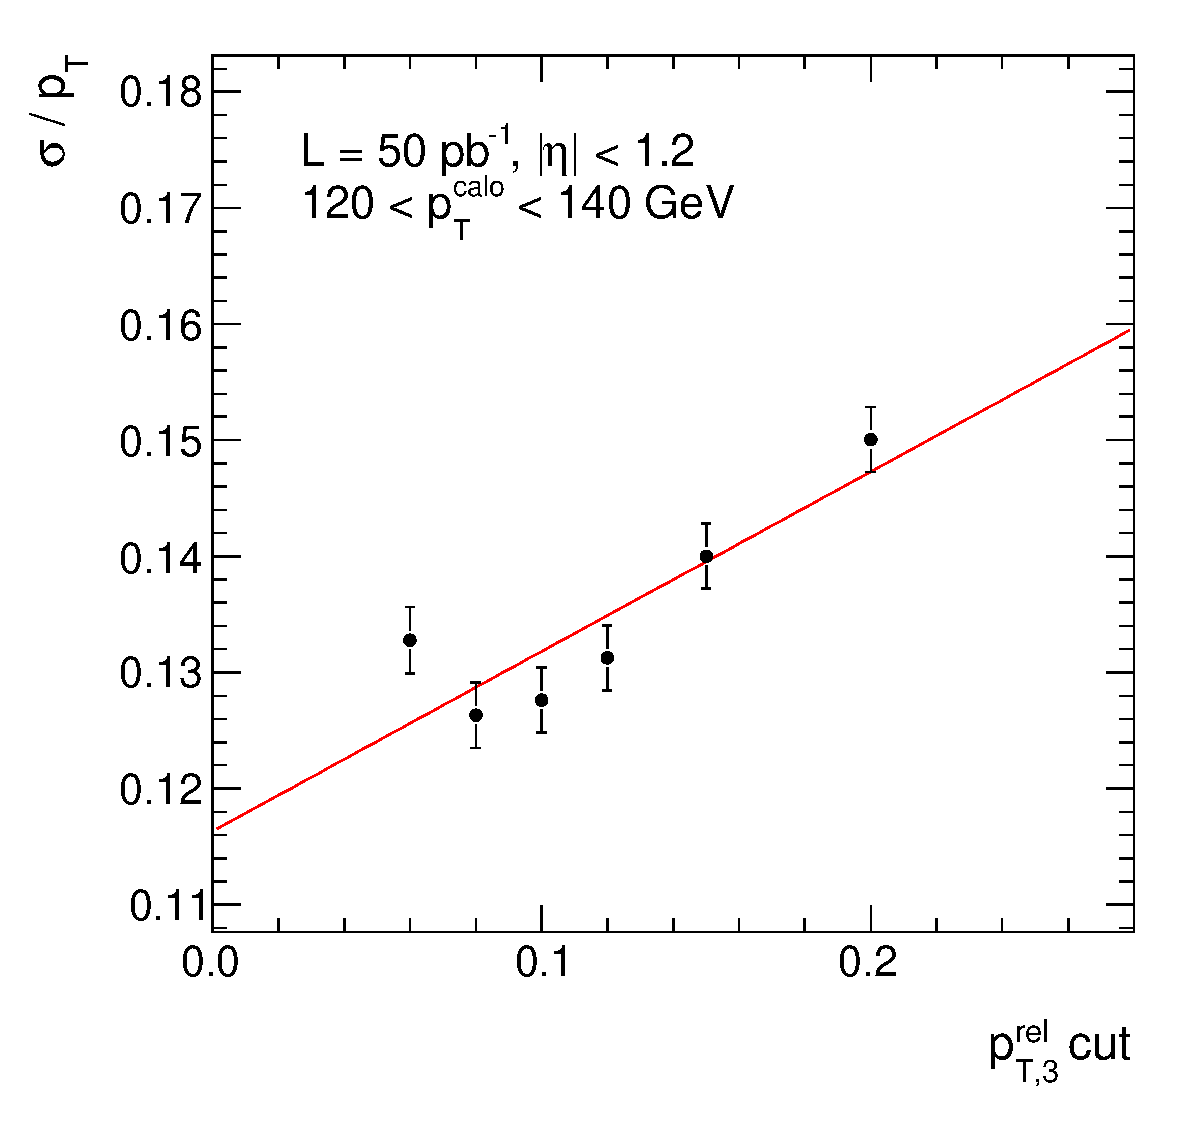
\includegraphics[width=0.3\textwidth]{figures/ResFit_Spring10QCDFlat_Gauss_Eta0_ExtrapolatedPar0_PtBin2} &
    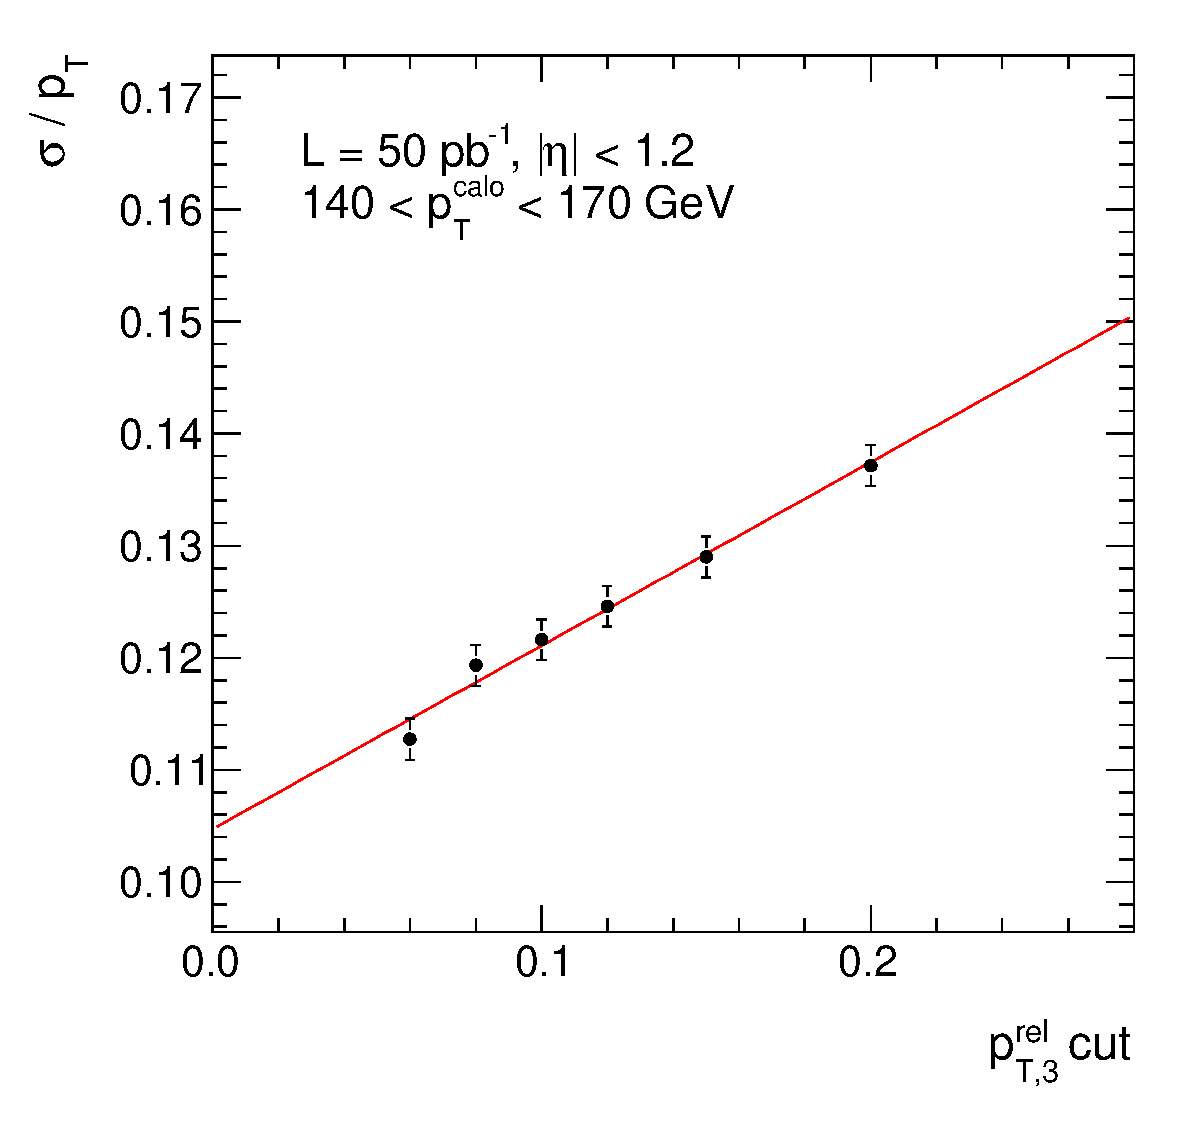
\includegraphics[width=0.3\textwidth]{figures/ResFit_Spring10QCDFlat_Gauss_Eta0_ExtrapolatedPar0_PtBin3} \\

    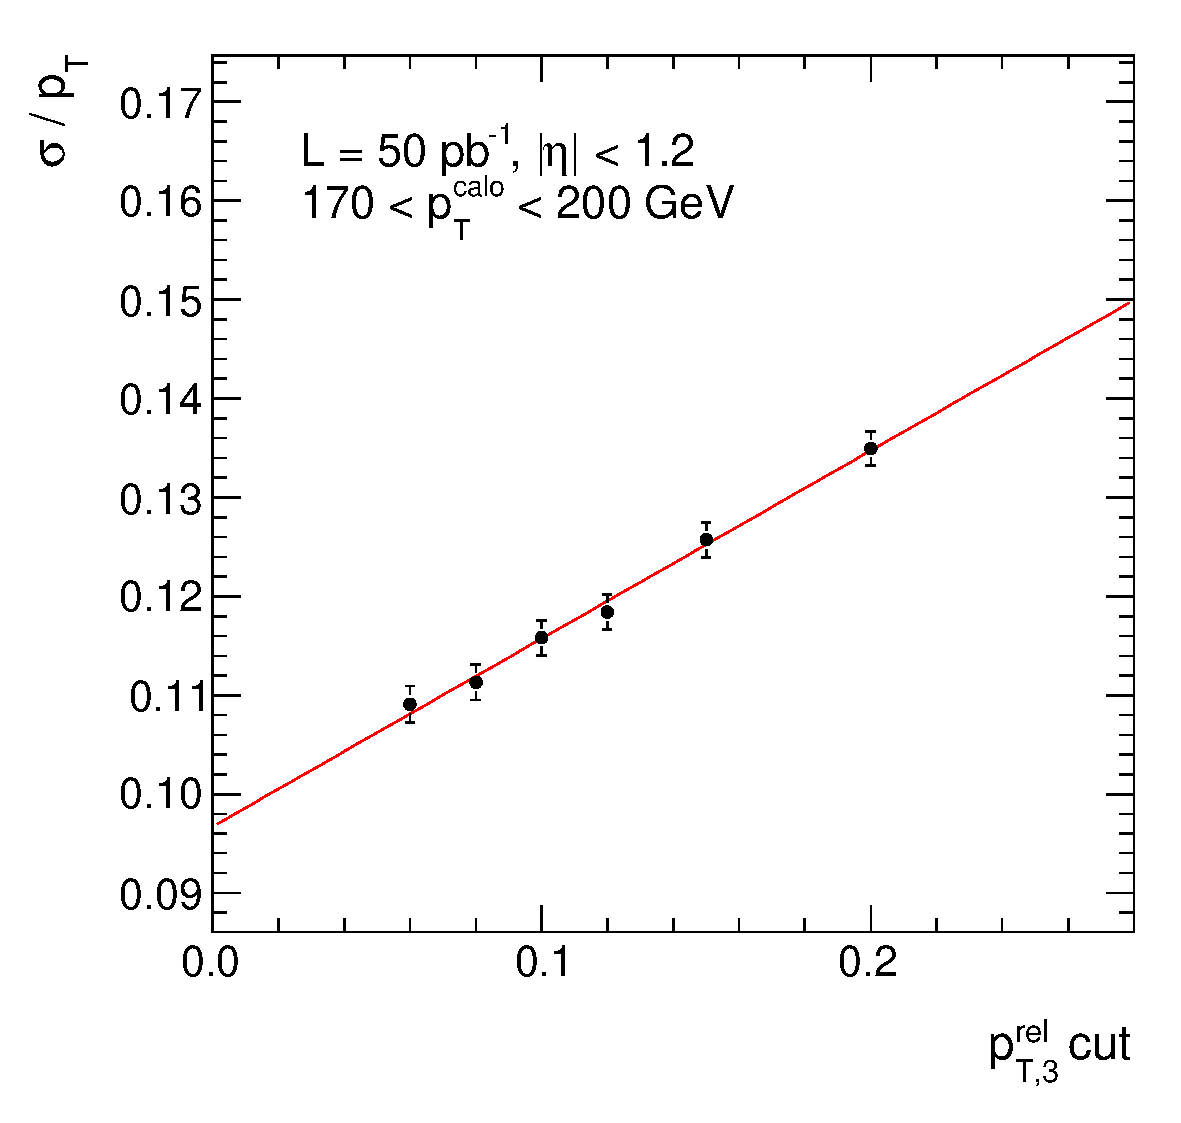
\includegraphics[width=0.3\textwidth]{figures/ResFit_Spring10QCDFlat_Gauss_Eta0_ExtrapolatedPar0_PtBin4} &
    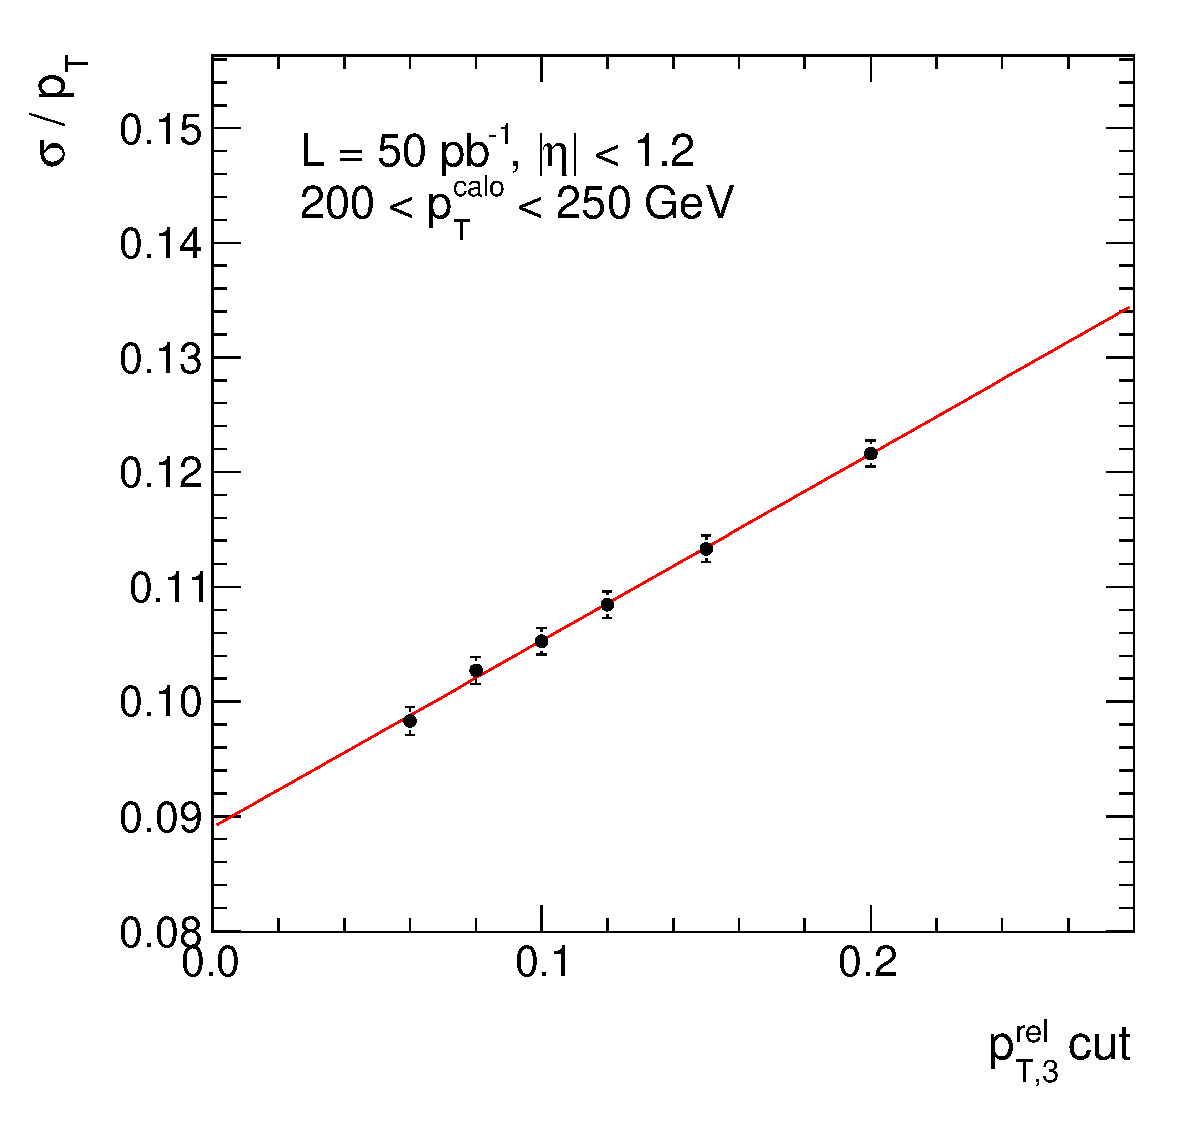
\includegraphics[width=0.3\textwidth]{figures/ResFit_Spring10QCDFlat_Gauss_Eta0_ExtrapolatedPar0_PtBin5} &
    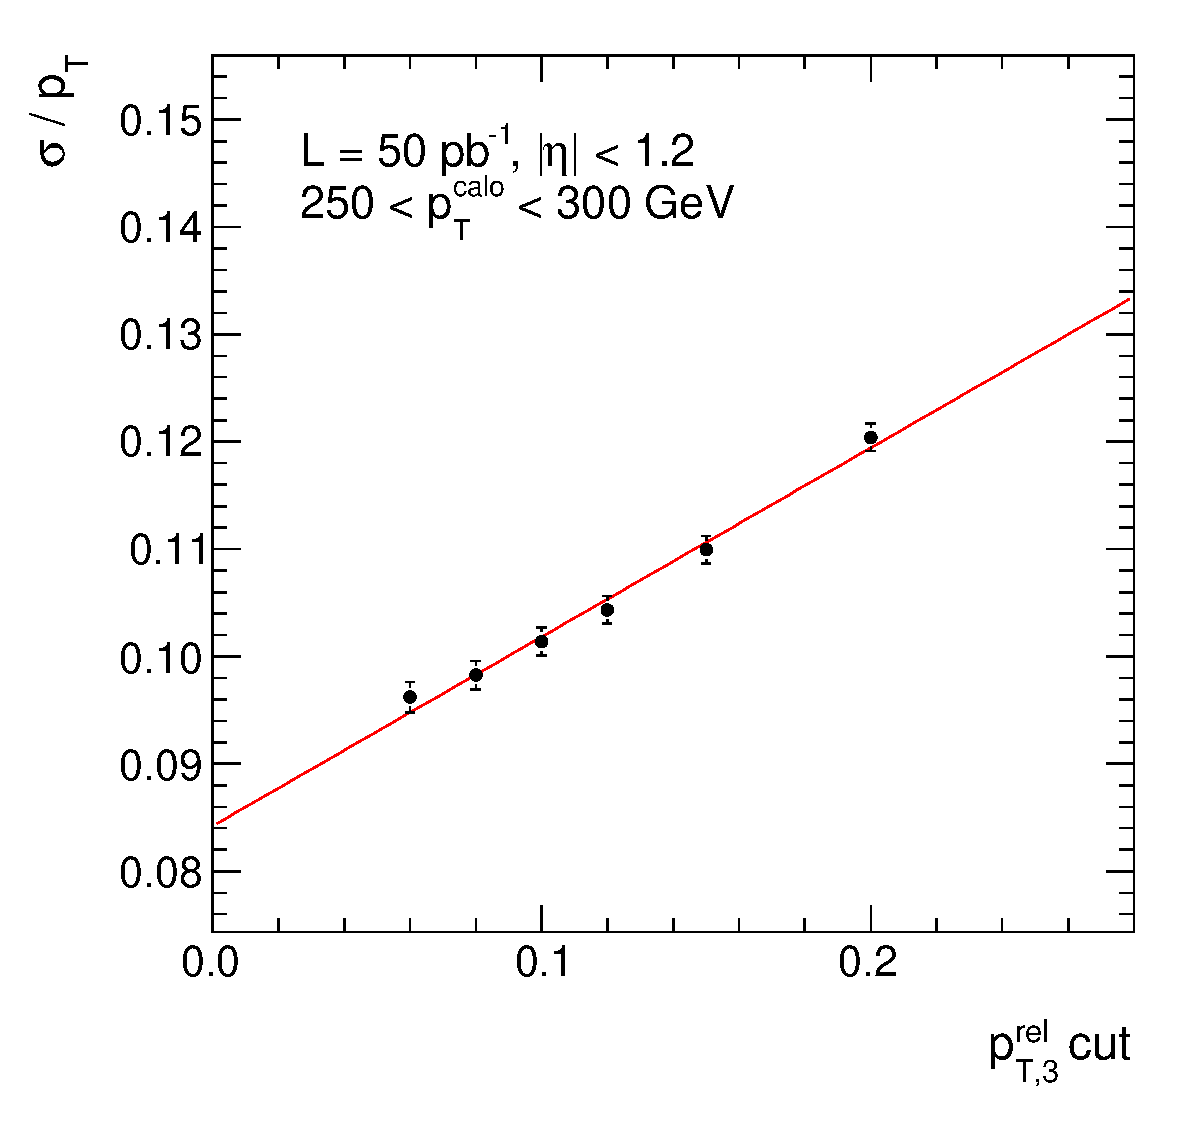
\includegraphics[width=0.3\textwidth]{figures/ResFit_Spring10QCDFlat_Gauss_Eta0_ExtrapolatedPar0_PtBin6} \\

    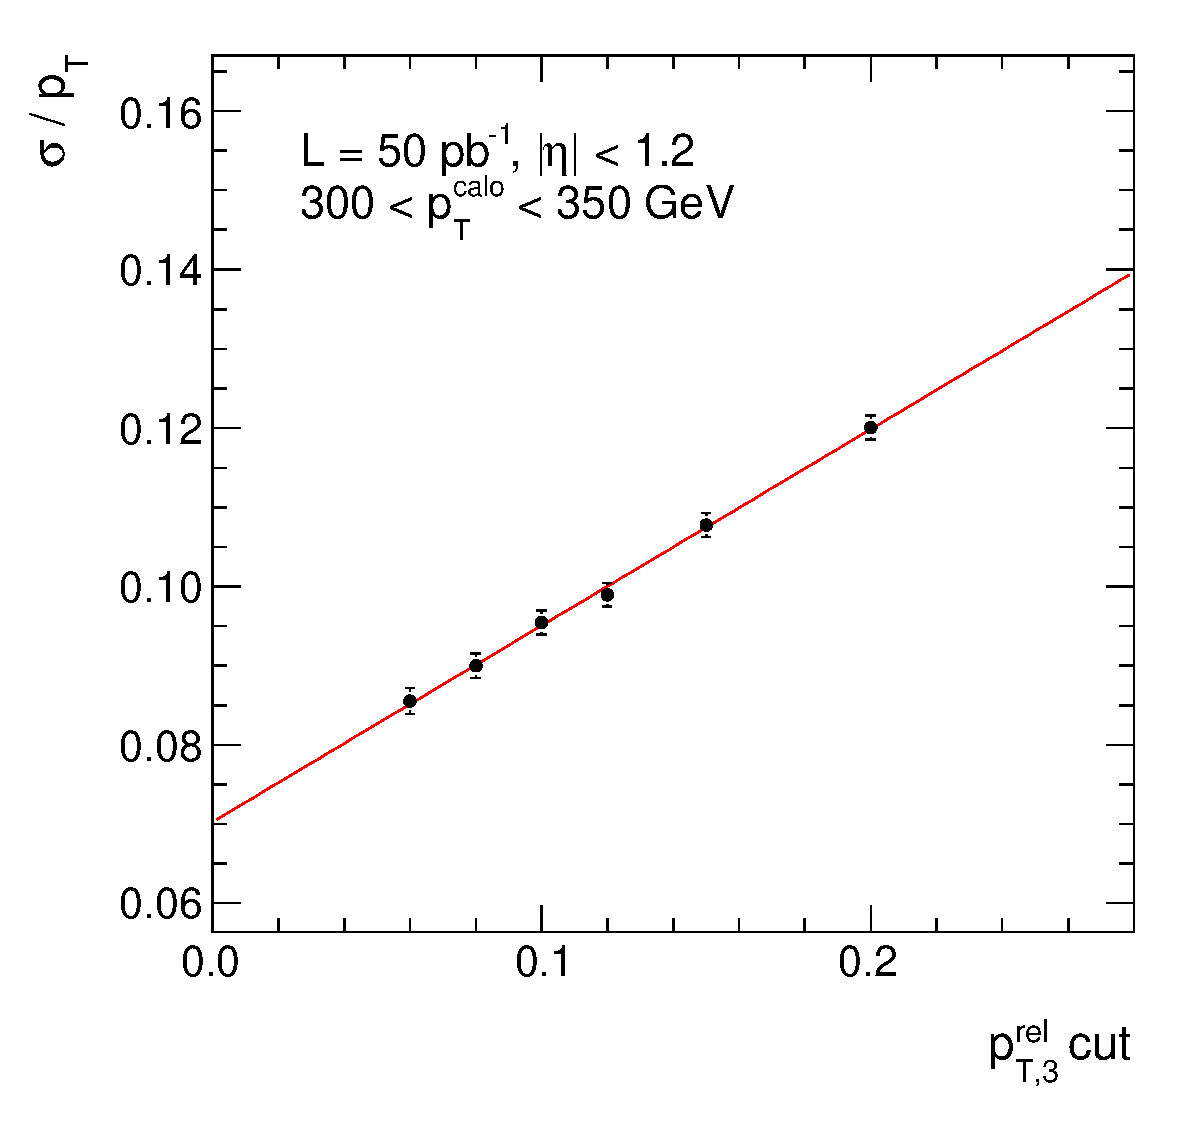
\includegraphics[width=0.3\textwidth]{figures/ResFit_Spring10QCDFlat_Gauss_Eta0_ExtrapolatedPar0_PtBin7} &
    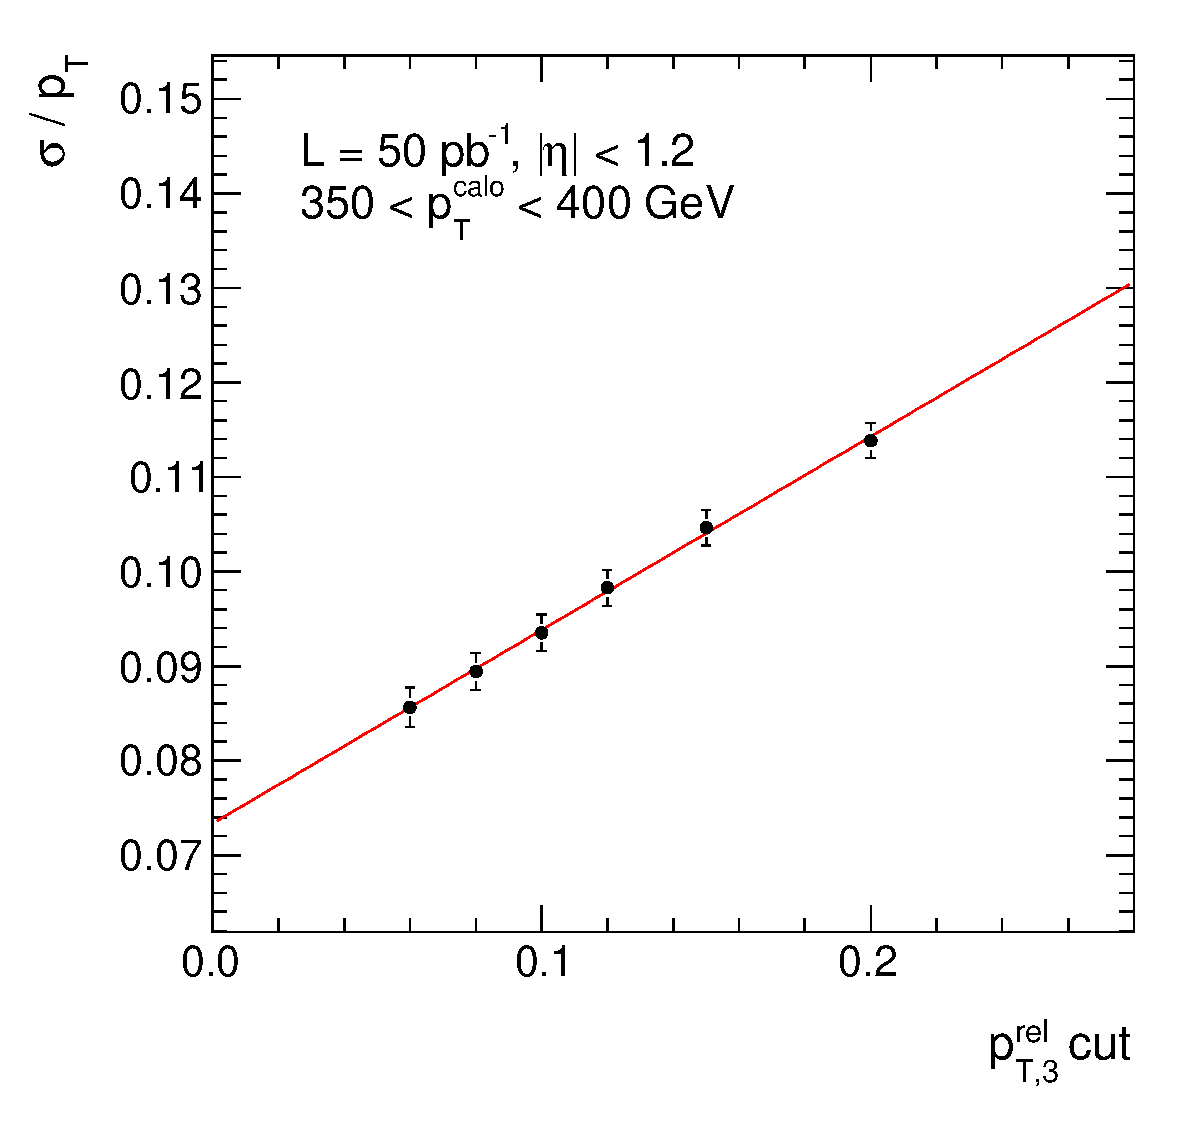
\includegraphics[width=0.3\textwidth]{figures/ResFit_Spring10QCDFlat_Gauss_Eta0_ExtrapolatedPar0_PtBin8} &
    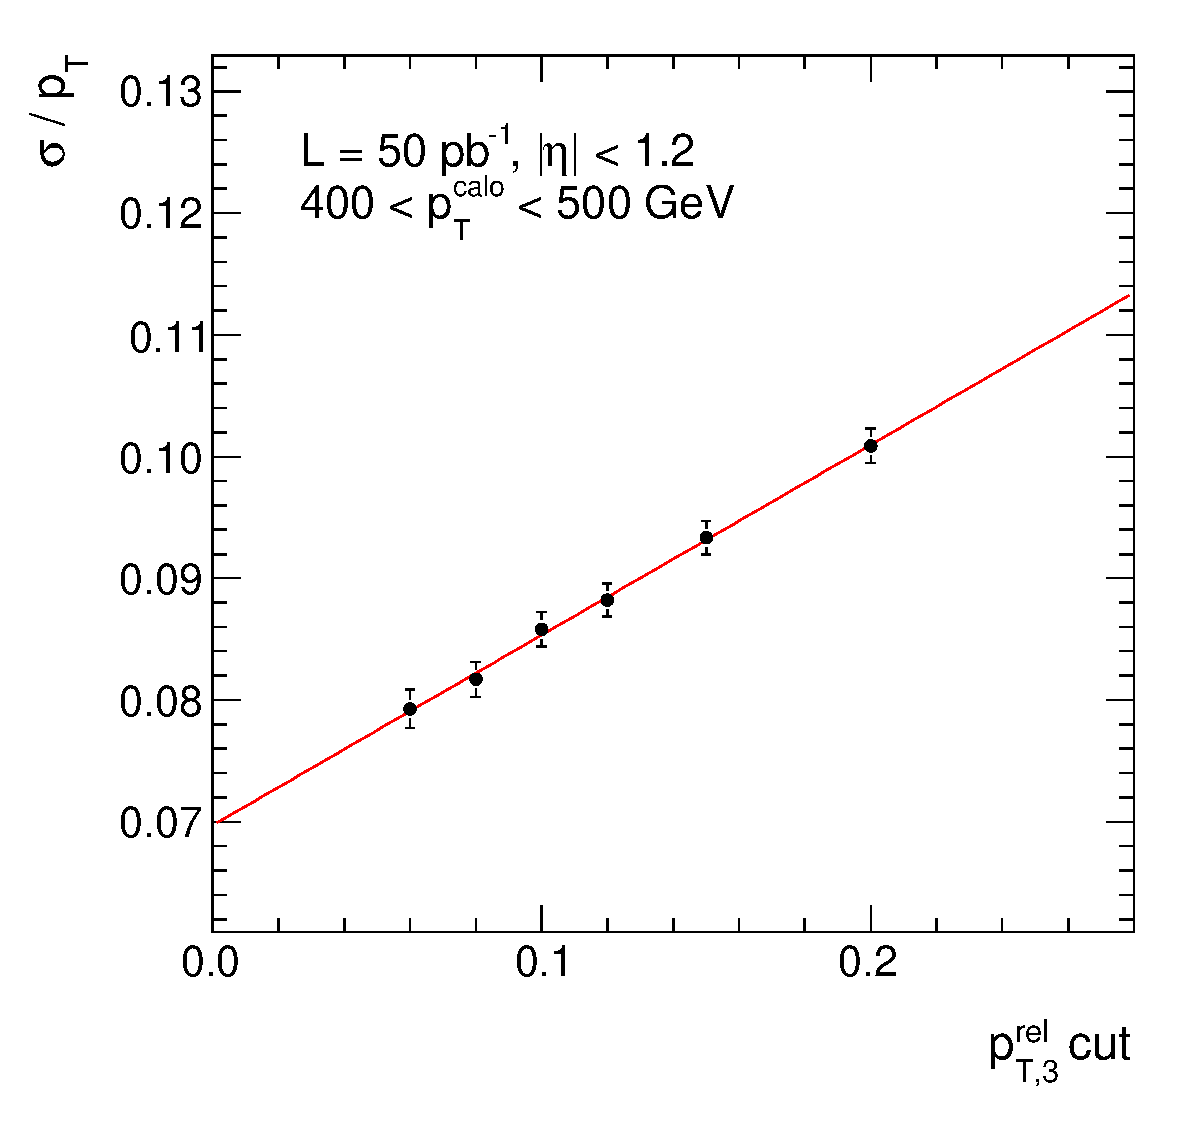
\includegraphics[width=0.3\textwidth]{figures/ResFit_Spring10QCDFlat_Gauss_Eta0_ExtrapolatedPar0_PtBin9} \\

    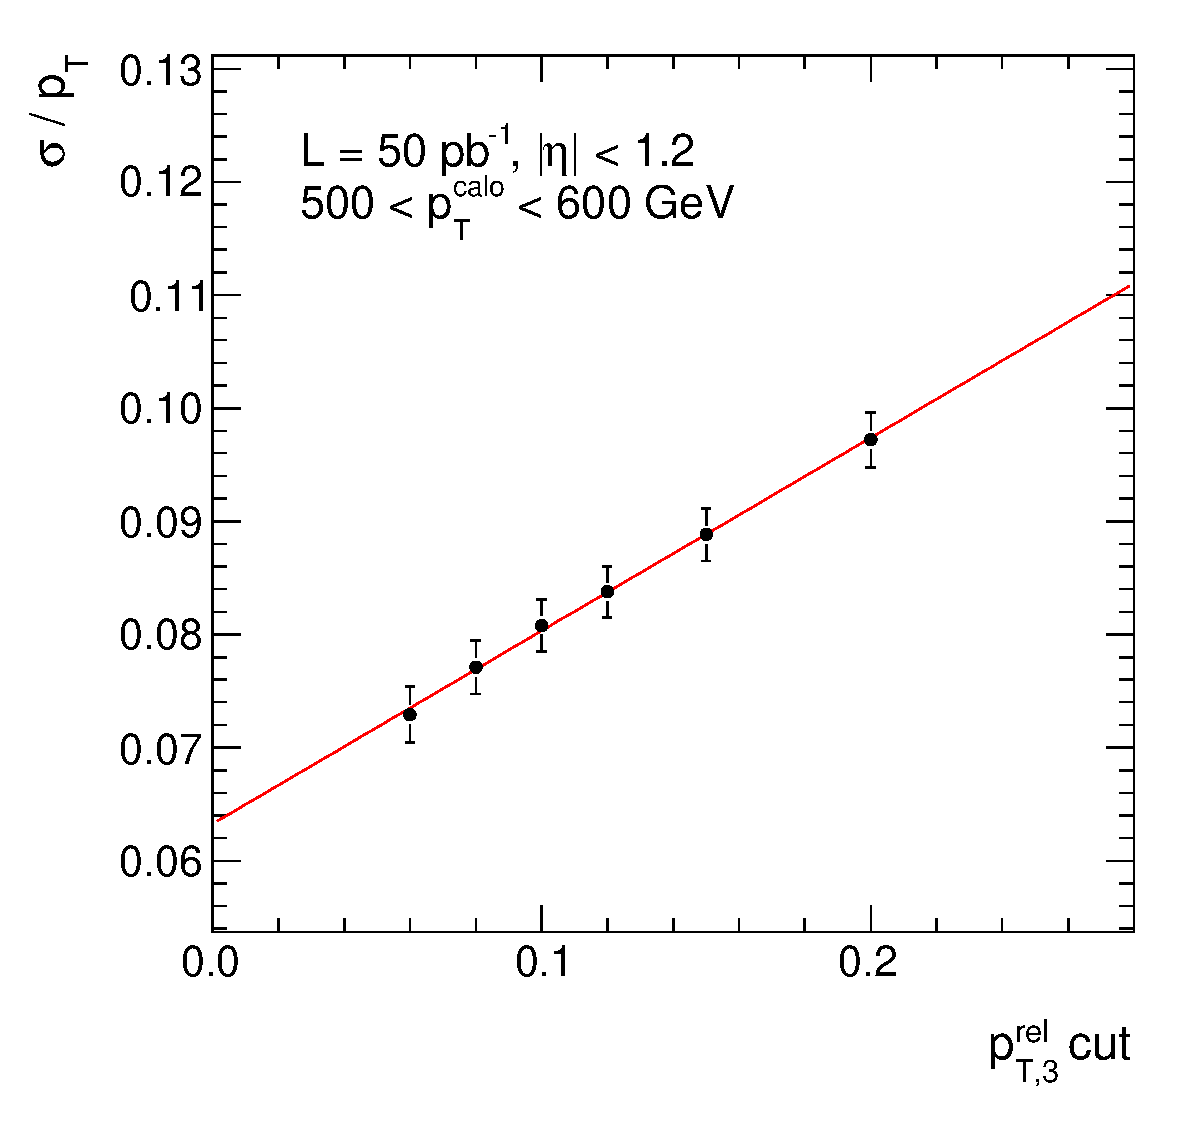
\includegraphics[width=0.3\textwidth]{figures/ResFit_Spring10QCDFlat_Gauss_Eta0_ExtrapolatedPar0_PtBin10} &
    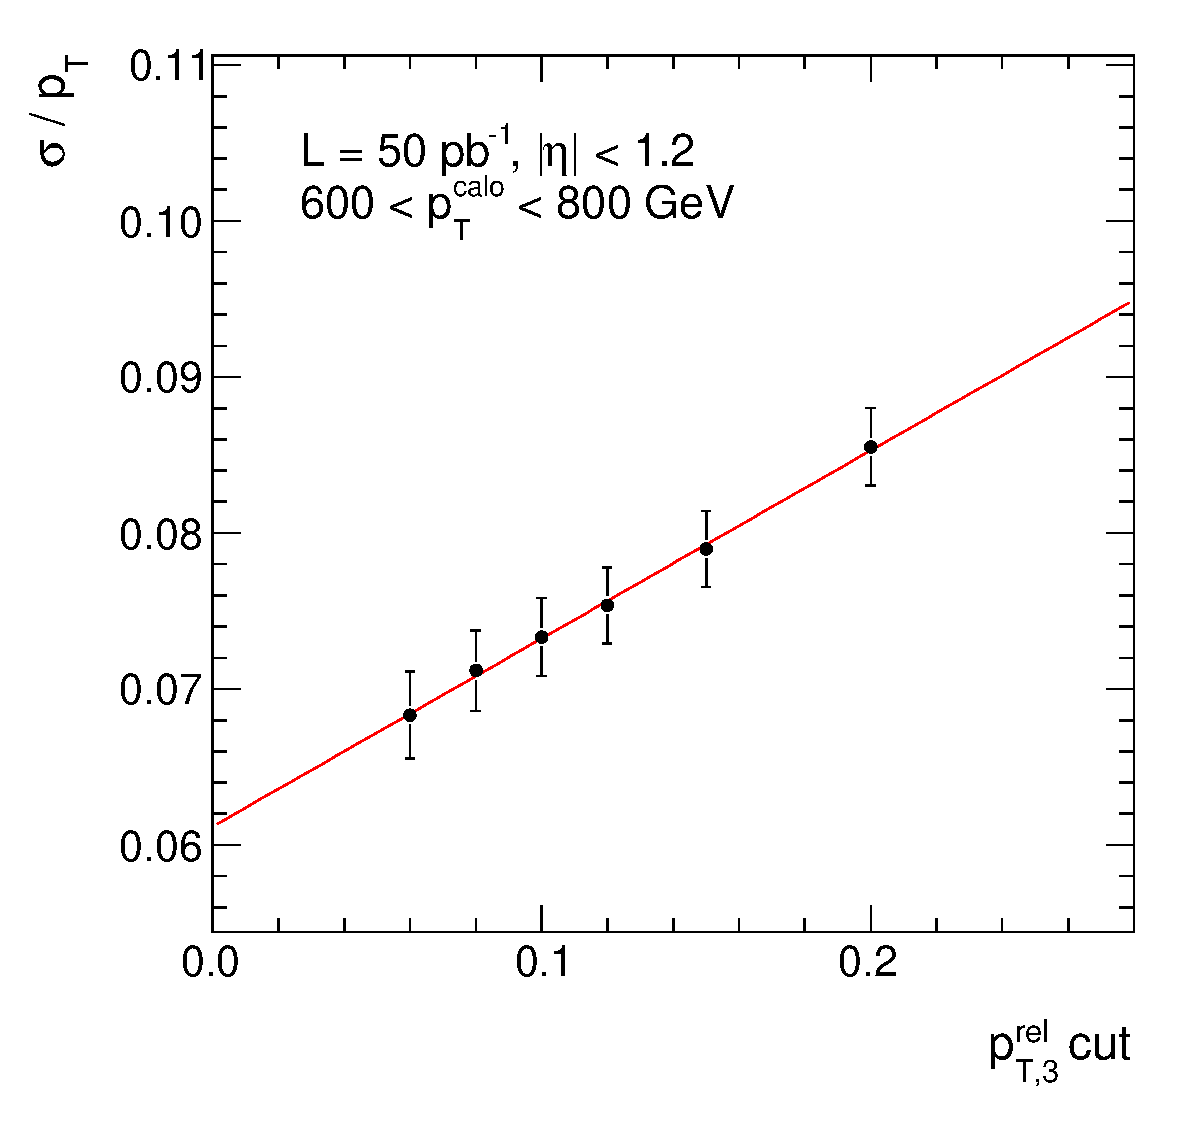
\includegraphics[width=0.3\textwidth]{figures/ResFit_Spring10QCDFlat_Gauss_Eta0_ExtrapolatedPar0_PtBin11} &
    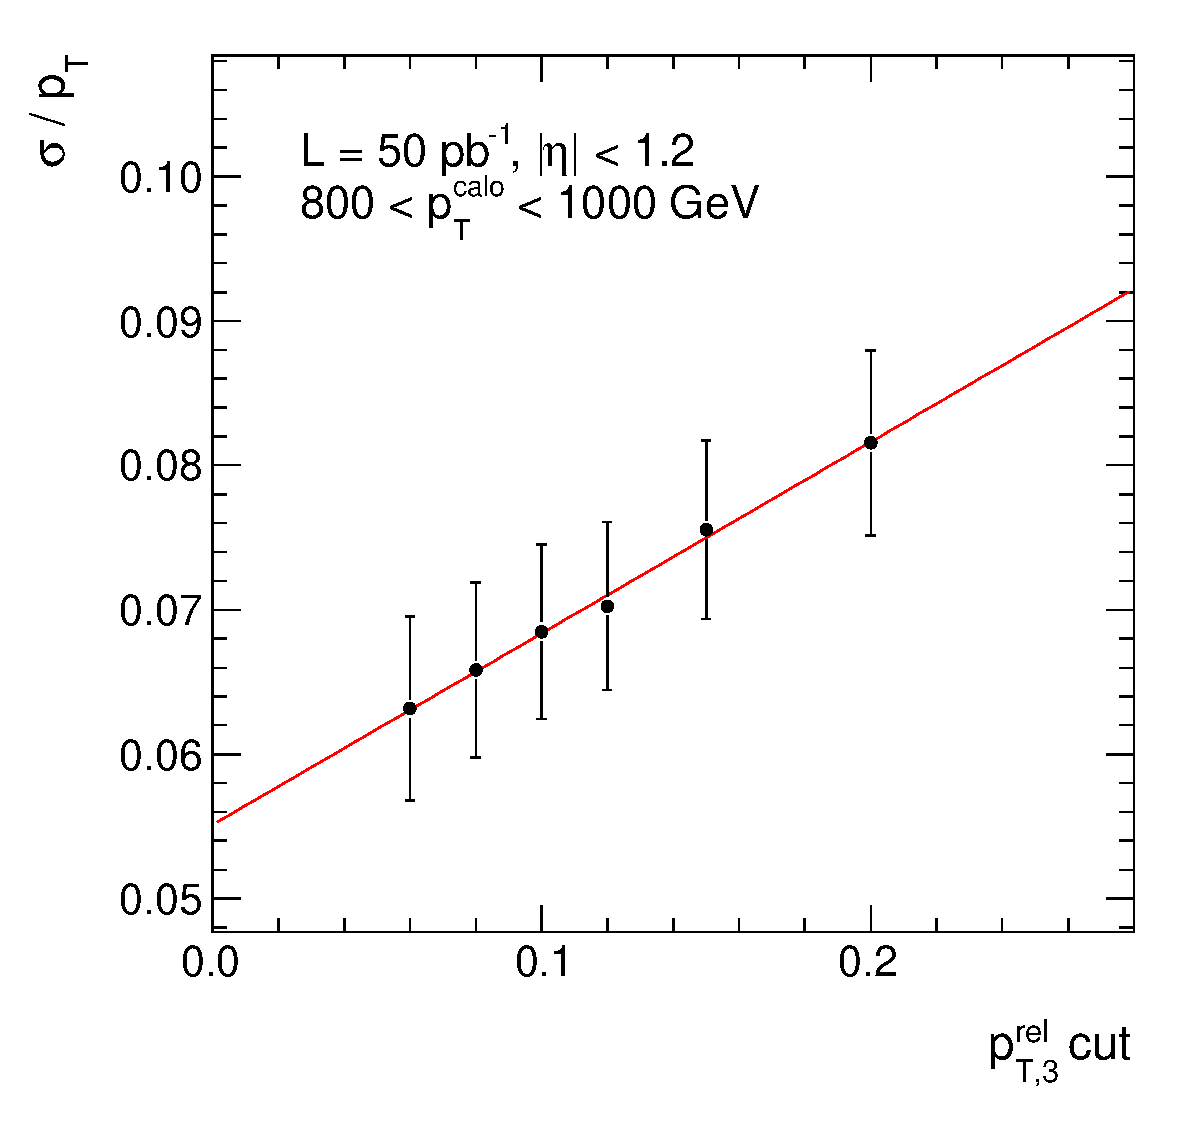
\includegraphics[width=0.3\textwidth]{figures/ResFit_Spring10QCDFlat_Gauss_Eta0_ExtrapolatedPar0_PtBin12} \\
  \end{tabular}
\caption{Resolutions $\bar{\sigma}/\pt$ from Gaussian fits for different limits on \ptrel in different \pt bins for \mbox{$|\eta|<1.2$}.
  The solid line is a linear fit to extrapolate $\bar{\sigma}/\pt$ to the ideal case of only two jets in the
  final state.}
\label{fig:ResFit:App:Gauss:Extrapolation}
\end{figure}


% ----- Gauss Eta0 MC truth closure -----
\begin{figure}[ht]
  \centering
  \begin{tabular}{ccc}
    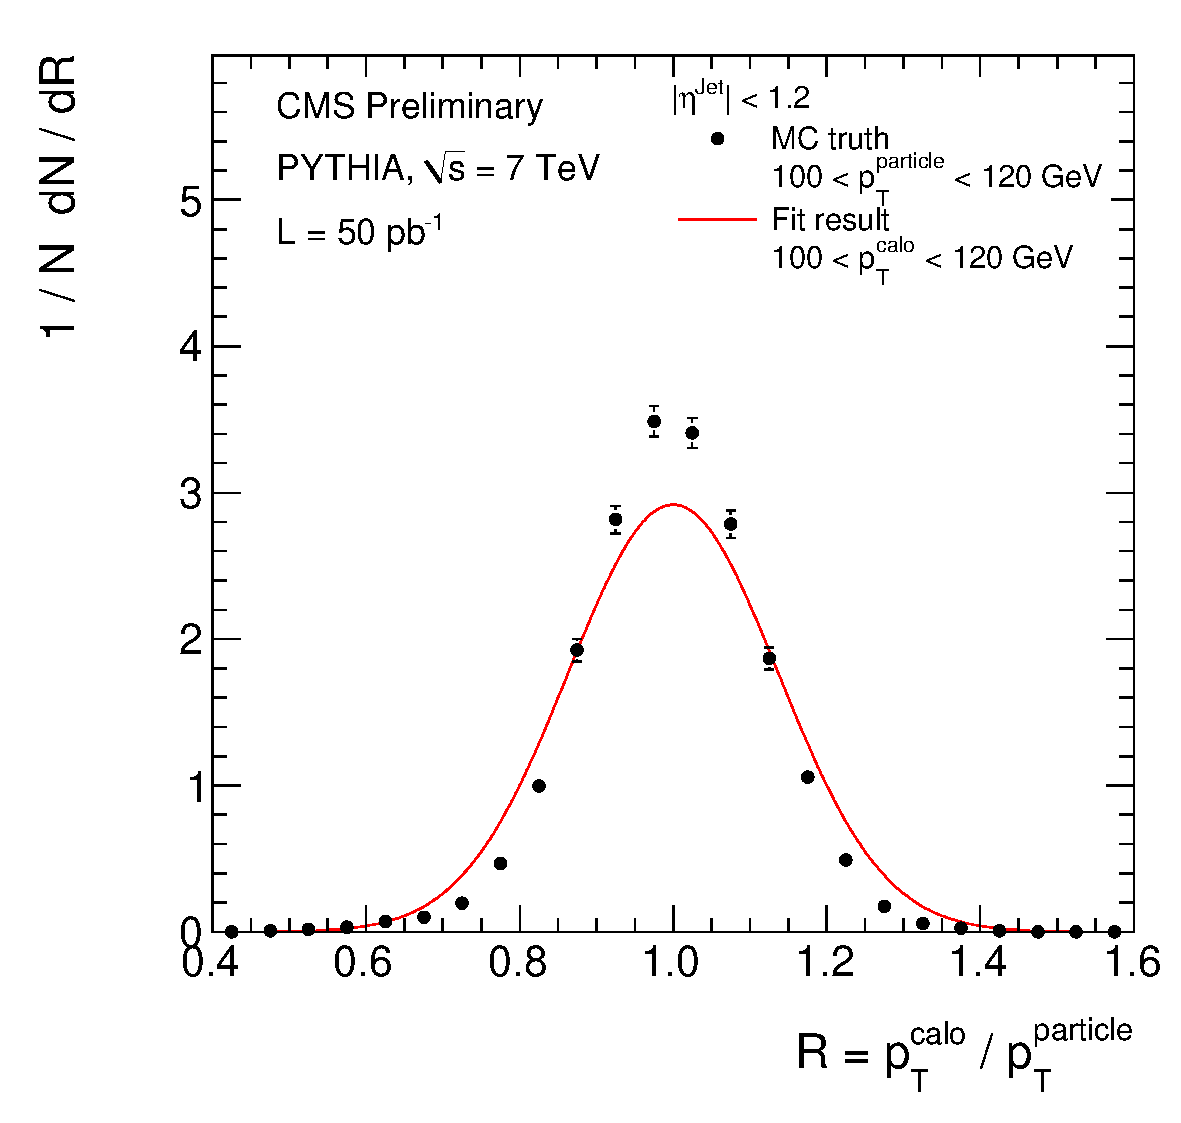
\includegraphics[width=0.3\textwidth]{figures/ResFit_Spring10QCDFlat_Gauss_Eta0_MCClosure_PtBin1} &
    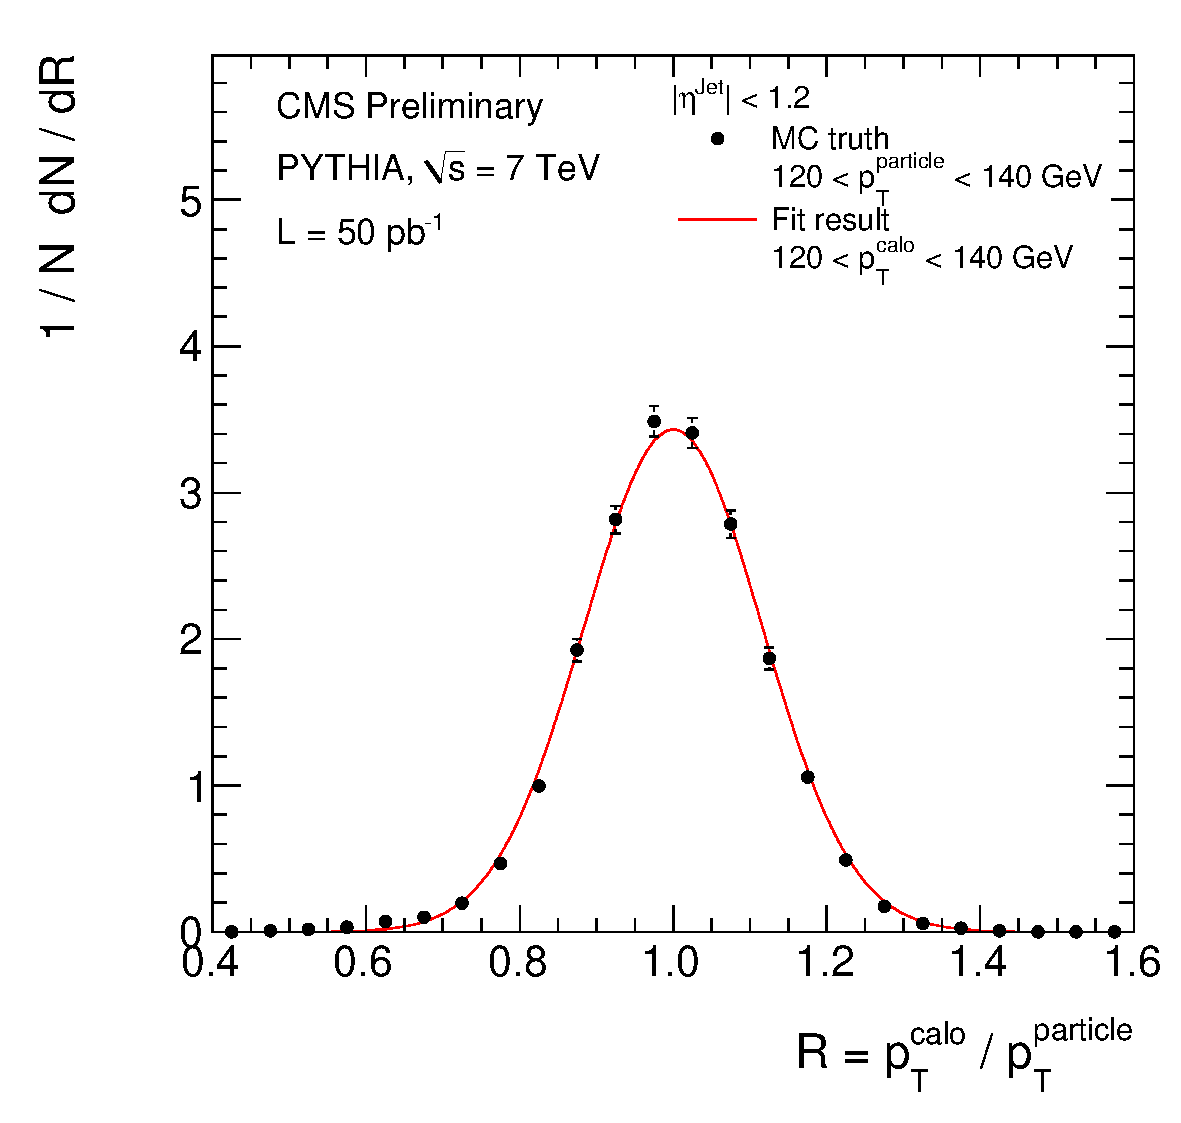
\includegraphics[width=0.3\textwidth]{figures/ResFit_Spring10QCDFlat_Gauss_Eta0_MCClosure_PtBin2} &
    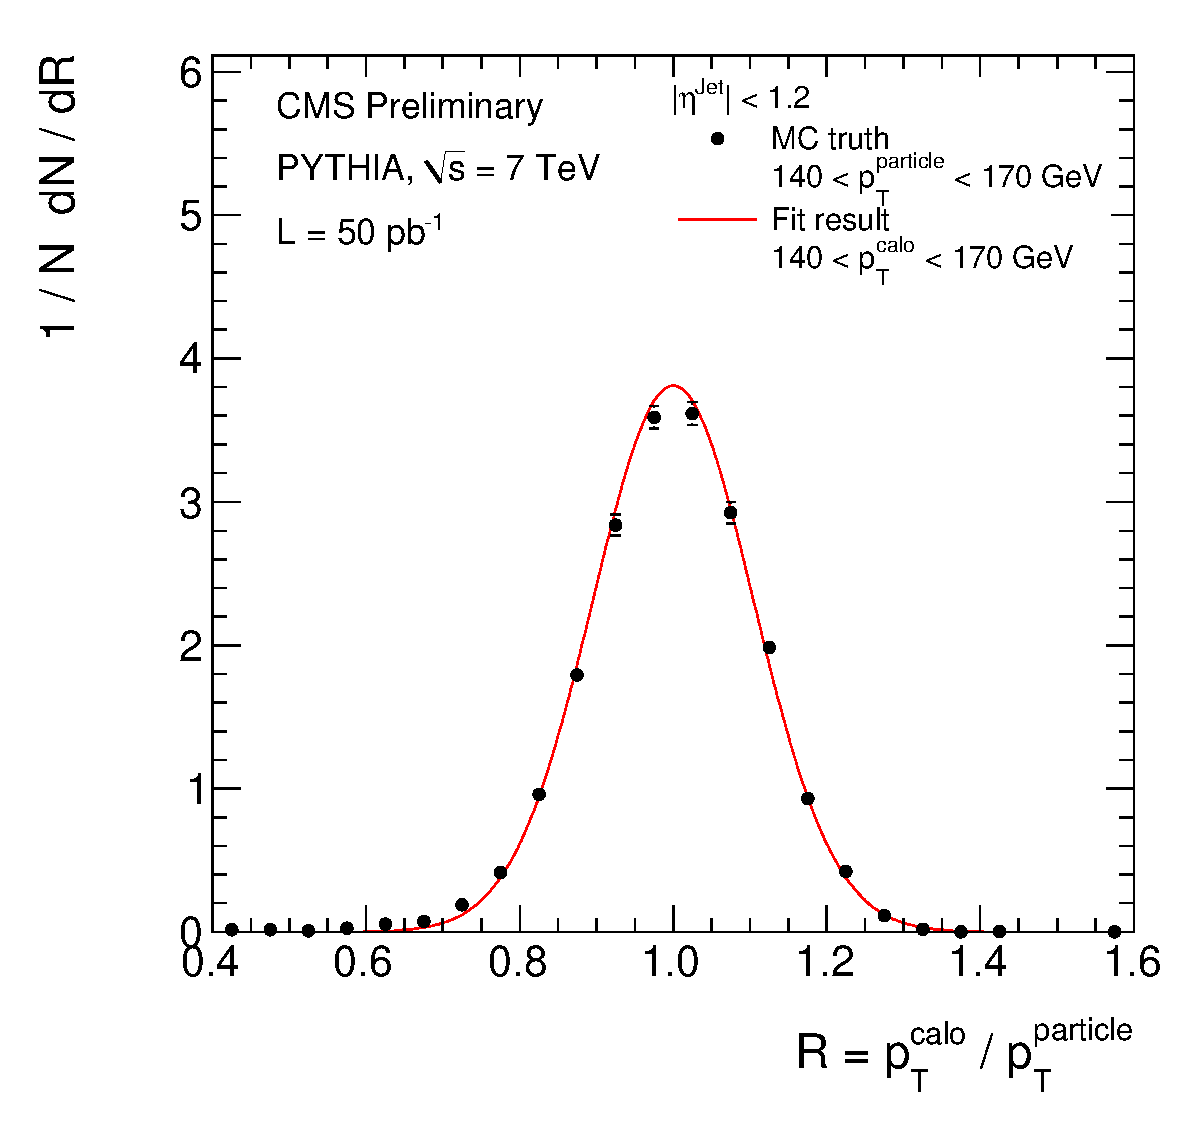
\includegraphics[width=0.3\textwidth]{figures/ResFit_Spring10QCDFlat_Gauss_Eta0_MCClosure_PtBin3} \\

    \includegraphics[width=0.3\textwidth]{figures/ResFit_Spring10QCDFlat_Gauss_Eta0_MCClosure_PtBin4} &
    \includegraphics[width=0.3\textwidth]{figures/ResFit_Spring10QCDFlat_Gauss_Eta0_MCClosure_PtBin5} &
    \includegraphics[width=0.3\textwidth]{figures/ResFit_Spring10QCDFlat_Gauss_Eta0_MCClosure_PtBin6} \\

    \includegraphics[width=0.3\textwidth]{figures/ResFit_Spring10QCDFlat_Gauss_Eta0_MCClosure_PtBin7} &
    \includegraphics[width=0.3\textwidth]{figures/ResFit_Spring10QCDFlat_Gauss_Eta0_MCClosure_PtBin8} &
    \includegraphics[width=0.3\textwidth]{figures/ResFit_Spring10QCDFlat_Gauss_Eta0_MCClosure_PtBin9} \\

    \includegraphics[width=0.3\textwidth]{figures/ResFit_Spring10QCDFlat_Gauss_Eta0_MCClosure_PtBin10} &
    \includegraphics[width=0.3\textwidth]{figures/ResFit_Spring10QCDFlat_Gauss_Eta0_MCClosure_PtBin11} &
    \includegraphics[width=0.3\textwidth]{figures/ResFit_Spring10QCDFlat_Gauss_Eta0_MCClosure_PtBin12} \\
  \end{tabular}
\caption{Closure \mbox{$|\eta|<1.2$}.}
\label{fig:ResFit:App:Gauss:MCClosure}
\end{figure}

\clearpage


\subsection{Crystal Ball response function}\label{sec:ResFit:App:AllResults:CrystalBall}

% ----- Crystal Ball Eta0 Spectra -----
\begin{figure}[ht]
  \centering
  \begin{tabular}{ccc}
    \includegraphics[width=0.3\textwidth]{figures/ResFit_Spring10QCDFlat_CB_Eta0_Spectrum_PtBin0} &
    \includegraphics[width=0.3\textwidth]{figures/ResFit_Spring10QCDFlat_CB_Eta0_Spectrum_PtBin1} &
    \includegraphics[width=0.3\textwidth]{figures/ResFit_Spring10QCDFlat_CB_Eta0_Spectrum_PtBin2} \\

    \includegraphics[width=0.3\textwidth]{figures/ResFit_Spring10QCDFlat_CB_Eta0_Spectrum_PtBin3} &
    \includegraphics[width=0.3\textwidth]{figures/ResFit_Spring10QCDFlat_CB_Eta0_Spectrum_PtBin4} &
    \includegraphics[width=0.3\textwidth]{figures/ResFit_Spring10QCDFlat_CB_Eta0_Spectrum_PtBin5} \\

    \includegraphics[width=0.3\textwidth]{figures/ResFit_Spring10QCDFlat_CB_Eta0_Spectrum_PtBin6} &
    \includegraphics[width=0.3\textwidth]{figures/ResFit_Spring10QCDFlat_CB_Eta0_Spectrum_PtBin7} &
    \includegraphics[width=0.3\textwidth]{figures/ResFit_Spring10QCDFlat_CB_Eta0_Spectrum_PtBin8} \\

    \includegraphics[width=0.3\textwidth]{figures/ResFit_Spring10QCDFlat_CB_Eta0_Spectrum_PtBin9} &
    \includegraphics[width=0.3\textwidth]{figures/ResFit_Spring10QCDFlat_CB_Eta0_Spectrum_PtBin10} & \\
  \end{tabular}
\caption{The parametrisation of the realistic particle jet \pt spectrum as used in the dijet likelihood (solid line) in comparison to the prediction from Monte Carlo truth (full circles) in different \pt bins for \mbox{$|\eta|<1.2$}. Migration effects are modelled assuming a Crystal Ball response function.}
\label{fig:ResFit:App:CB:Spectrum}
\end{figure}


% ----- Crystal Ball Eta0 extrapolations -----
\begin{figure}[ht]
  \centering
  \begin{tabular}{ccc}
    \includegraphics[width=0.3\textwidth]{figures/ResFit_Spring10QCDFlat_CB_Eta0_ExtrapolatedPar0_PtBin0} &
    \includegraphics[width=0.3\textwidth]{figures/ResFit_Spring10QCDFlat_CB_Eta0_ExtrapolatedPar0_PtBin1} &
    \includegraphics[width=0.3\textwidth]{figures/ResFit_Spring10QCDFlat_CB_Eta0_ExtrapolatedPar0_PtBin2} \\

    \includegraphics[width=0.3\textwidth]{figures/ResFit_Spring10QCDFlat_CB_Eta0_ExtrapolatedPar0_PtBin3} &
    \includegraphics[width=0.3\textwidth]{figures/ResFit_Spring10QCDFlat_CB_Eta0_ExtrapolatedPar0_PtBin4} &
    \includegraphics[width=0.3\textwidth]{figures/ResFit_Spring10QCDFlat_CB_Eta0_ExtrapolatedPar0_PtBin5} \\

    \includegraphics[width=0.3\textwidth]{figures/ResFit_Spring10QCDFlat_CB_Eta0_ExtrapolatedPar0_PtBin6} &
    \includegraphics[width=0.3\textwidth]{figures/ResFit_Spring10QCDFlat_CB_Eta0_ExtrapolatedPar0_PtBin7} &
    \includegraphics[width=0.3\textwidth]{figures/ResFit_Spring10QCDFlat_CB_Eta0_ExtrapolatedPar0_PtBin8} \\

    \includegraphics[width=0.3\textwidth]{figures/ResFit_Spring10QCDFlat_CB_Eta0_ExtrapolatedPar0_PtBin9} &
    \includegraphics[width=0.3\textwidth]{figures/ResFit_Spring10QCDFlat_CB_Eta0_ExtrapolatedPar0_PtBin10} & \\
  \end{tabular}
\caption{}
\label{fig:ResFit:App:CB:ExtrapolatedPar0}
\end{figure}

\begin{figure}[ht]
  \centering
  \begin{tabular}{ccc}
    \includegraphics[width=0.3\textwidth]{figures/ResFit_Spring10QCDFlat_CB_Eta0_ExtrapolatedPar1_PtBin0} &
    \includegraphics[width=0.3\textwidth]{figures/ResFit_Spring10QCDFlat_CB_Eta0_ExtrapolatedPar1_PtBin1} &
    \includegraphics[width=0.3\textwidth]{figures/ResFit_Spring10QCDFlat_CB_Eta0_ExtrapolatedPar1_PtBin2} \\

    \includegraphics[width=0.3\textwidth]{figures/ResFit_Spring10QCDFlat_CB_Eta0_ExtrapolatedPar1_PtBin3} &
    \includegraphics[width=0.3\textwidth]{figures/ResFit_Spring10QCDFlat_CB_Eta0_ExtrapolatedPar1_PtBin4} &
    \includegraphics[width=0.3\textwidth]{figures/ResFit_Spring10QCDFlat_CB_Eta0_ExtrapolatedPar1_PtBin5} \\

    \includegraphics[width=0.3\textwidth]{figures/ResFit_Spring10QCDFlat_CB_Eta0_ExtrapolatedPar1_PtBin6} &
    \includegraphics[width=0.3\textwidth]{figures/ResFit_Spring10QCDFlat_CB_Eta0_ExtrapolatedPar1_PtBin7} &
    \includegraphics[width=0.3\textwidth]{figures/ResFit_Spring10QCDFlat_CB_Eta0_ExtrapolatedPar1_PtBin8} \\

    \includegraphics[width=0.3\textwidth]{figures/ResFit_Spring10QCDFlat_CB_Eta0_ExtrapolatedPar1_PtBin9} &
    \includegraphics[width=0.3\textwidth]{figures/ResFit_Spring10QCDFlat_CB_Eta0_ExtrapolatedPar1_PtBin10} & \\
  \end{tabular}
\caption{}
\label{fig:ResFit:App:CB:ExtrapolatedPar1}
\end{figure}

\begin{figure}[ht]
  \centering
  \begin{tabular}{ccc}
    \includegraphics[width=0.3\textwidth]{figures/ResFit_Spring10QCDFlat_CB_Eta0_ExtrapolatedPar2_PtBin0} &
    \includegraphics[width=0.3\textwidth]{figures/ResFit_Spring10QCDFlat_CB_Eta0_ExtrapolatedPar2_PtBin1} &
    \includegraphics[width=0.3\textwidth]{figures/ResFit_Spring10QCDFlat_CB_Eta0_ExtrapolatedPar2_PtBin2} \\

    \includegraphics[width=0.3\textwidth]{figures/ResFit_Spring10QCDFlat_CB_Eta0_ExtrapolatedPar2_PtBin3} &
    \includegraphics[width=0.3\textwidth]{figures/ResFit_Spring10QCDFlat_CB_Eta0_ExtrapolatedPar2_PtBin4} &
    \includegraphics[width=0.3\textwidth]{figures/ResFit_Spring10QCDFlat_CB_Eta0_ExtrapolatedPar2_PtBin5} \\

    \includegraphics[width=0.3\textwidth]{figures/ResFit_Spring10QCDFlat_CB_Eta0_ExtrapolatedPar2_PtBin6} &
    \includegraphics[width=0.3\textwidth]{figures/ResFit_Spring10QCDFlat_CB_Eta0_ExtrapolatedPar2_PtBin7} &
    \includegraphics[width=0.3\textwidth]{figures/ResFit_Spring10QCDFlat_CB_Eta0_ExtrapolatedPar2_PtBin8} \\

    \includegraphics[width=0.3\textwidth]{figures/ResFit_Spring10QCDFlat_CB_Eta0_ExtrapolatedPar2_PtBin9} &
    \includegraphics[width=0.3\textwidth]{figures/ResFit_Spring10QCDFlat_CB_Eta0_ExtrapolatedPar2_PtBin10} & \\
  \end{tabular}
\caption{}
\label{fig:ResFit:App:CB:ExtrapolatedPar2}
\end{figure}


% ----- Crystal Ball Eta0 MCClosure -----
\begin{figure}[ht]
  \centering
  \begin{tabular}{ccc}
    \includegraphics[width=0.3\textwidth]{figures/ResFit_Spring10QCDFlat_CB_Eta0_MCClosure_PtBin0} &
    \includegraphics[width=0.3\textwidth]{figures/ResFit_Spring10QCDFlat_CB_Eta0_MCClosure_PtBin1} &
    \includegraphics[width=0.3\textwidth]{figures/ResFit_Spring10QCDFlat_CB_Eta0_MCClosure_PtBin2} \\

    \includegraphics[width=0.3\textwidth]{figures/ResFit_Spring10QCDFlat_CB_Eta0_MCClosure_PtBin3} &
    \includegraphics[width=0.3\textwidth]{figures/ResFit_Spring10QCDFlat_CB_Eta0_MCClosure_PtBin4} &
    \includegraphics[width=0.3\textwidth]{figures/ResFit_Spring10QCDFlat_CB_Eta0_MCClosure_PtBin5} \\

    \includegraphics[width=0.3\textwidth]{figures/ResFit_Spring10QCDFlat_CB_Eta0_MCClosure_PtBin6} &
    \includegraphics[width=0.3\textwidth]{figures/ResFit_Spring10QCDFlat_CB_Eta0_MCClosure_PtBin7} &
    \includegraphics[width=0.3\textwidth]{figures/ResFit_Spring10QCDFlat_CB_Eta0_MCClosure_PtBin8} \\

    \includegraphics[width=0.3\textwidth]{figures/ResFit_Spring10QCDFlat_CB_Eta0_MCClosure_PtBin9} &
    \includegraphics[width=0.3\textwidth]{figures/ResFit_Spring10QCDFlat_CB_Eta0_MCClosure_PtBin10} & \\
  \end{tabular}
\caption{Closure \mbox{$|\eta|<1.2$}.}
\label{fig:ResFit:App:CB:MCClosure}
\end{figure}

\clearpage



% ----- Bibliography ------------------------------------

\begin{thebibliography}{9}
\bibitem{bib:ra2} The CMS SUSY RA2 Group,
  \textit{Inclusive search for SUSY at CMS with the jets plus missing
    momentum signature},
  CMS AN~2010/260 (2010).
\bibitem{bib:asym} C.~Dragoiu \etal,
  \textit{Measurement of the Jet Energy Resolution in $\sqrt{s}=7\tev$
    Collision Data with the Asymmetry Method},
  CMS AN~2010/134 (2010).
\bibitem{bib:cmspas:monster} The CMS Collaboration,
  \textit{Transverse Momentum and Pseudorapidity Distributions of
    Charged Hadrons in $pp$ Collisions at \mbox{$\sqrt{s} = 0.9$} and $2.36\tev$}, JHEP 02 (2010) 041,
 xarXiv:1002.0621. doi:10.1007/JHEP02(2010)041.
\bibitem{bib:cmspas:vertex} The CMS Collaboration,
  \textit{Tracking and Primary Vertex Results in First $7\tev$ Collisions},
  CMS PAS TRK-10-005 (2010).
\bibitem{bib:pythia} T.~Sj\o"strand \etal,
  \textit{PYTHIA 6.4 physics and manual},
  JHEP05(2006)026. doi:10.1088/1126-6708/2006/05/026.
\bibitem{bib:geant} GEANT4 Collaboration,
  \textit{GEANT4: A simulation toolkit},
  Nucl. Instrum. and Methods A506 (2003) 250-303. doi:10.1016/S0168-9002(03)01368-8.
\bibitem{bib:akj} M.~Cacciari, G.~P.~Salam, and G.~Soyez,
  \textit{The anti-kt jet clustering algorithm},
  JHEP~0804:063 (2008).
\bibitem{bib:cmspas:jec} The CMS Collaboration,
  \textit{Plans for Jet Energy Corrections at CMS},
  CMS PAS JME-07-002 (2007).
\bibitem{bib:cmspas:jetid}  The CMS Collaboration,
  \textit{Calorimeter Jet Quality Criteria for the First CMS Collision Data},
  CMS PAS JME-09-008 (2008).
%\bibitem{bib:cmsan:mcjer} R.~Ciesielski \etal,
%  \textit{Jet Energy Resolutions Derived from QCD Simulation for the Analysis of First $\sqrt{s}=7\,\mathrm{TeV}$ Collision Data},
%  CMS AN 2010/121 (2010).
\end{thebibliography}



\end{document}
